\section{Familias de Optimizadores}
\label{sec:annex-optimizers}

\subsection{La Evolución de la Optimización en Redes Neuronales}
El estudio de optimizadores enmarca la optimización de transformadores como una respuesta a tres presiones estructurales: paisajes de pérdida no convexos, heterogeneidad severa de curvatura entre bloques de parámetros y el costo de memoria de almacenar el estado del optimizador para modelos muy grandes. El informe sostiene que el campo se ha diversificado en varias trayectorias: líneas base adaptativas de primer orden, métodos de reducción de varianza, métodos eficientes en memoria, precondicionadores estructurados de segundo orden, métodos sin programación de tasa de aprendizaje y actualizaciones orientadas a ortogonalidad.

\subsection{Línea Base Estándar y Optimizadores Adaptativos}
\paragraph{SGD con Momentum.}
\begin{figure}[H]
\centering
\fitfigure{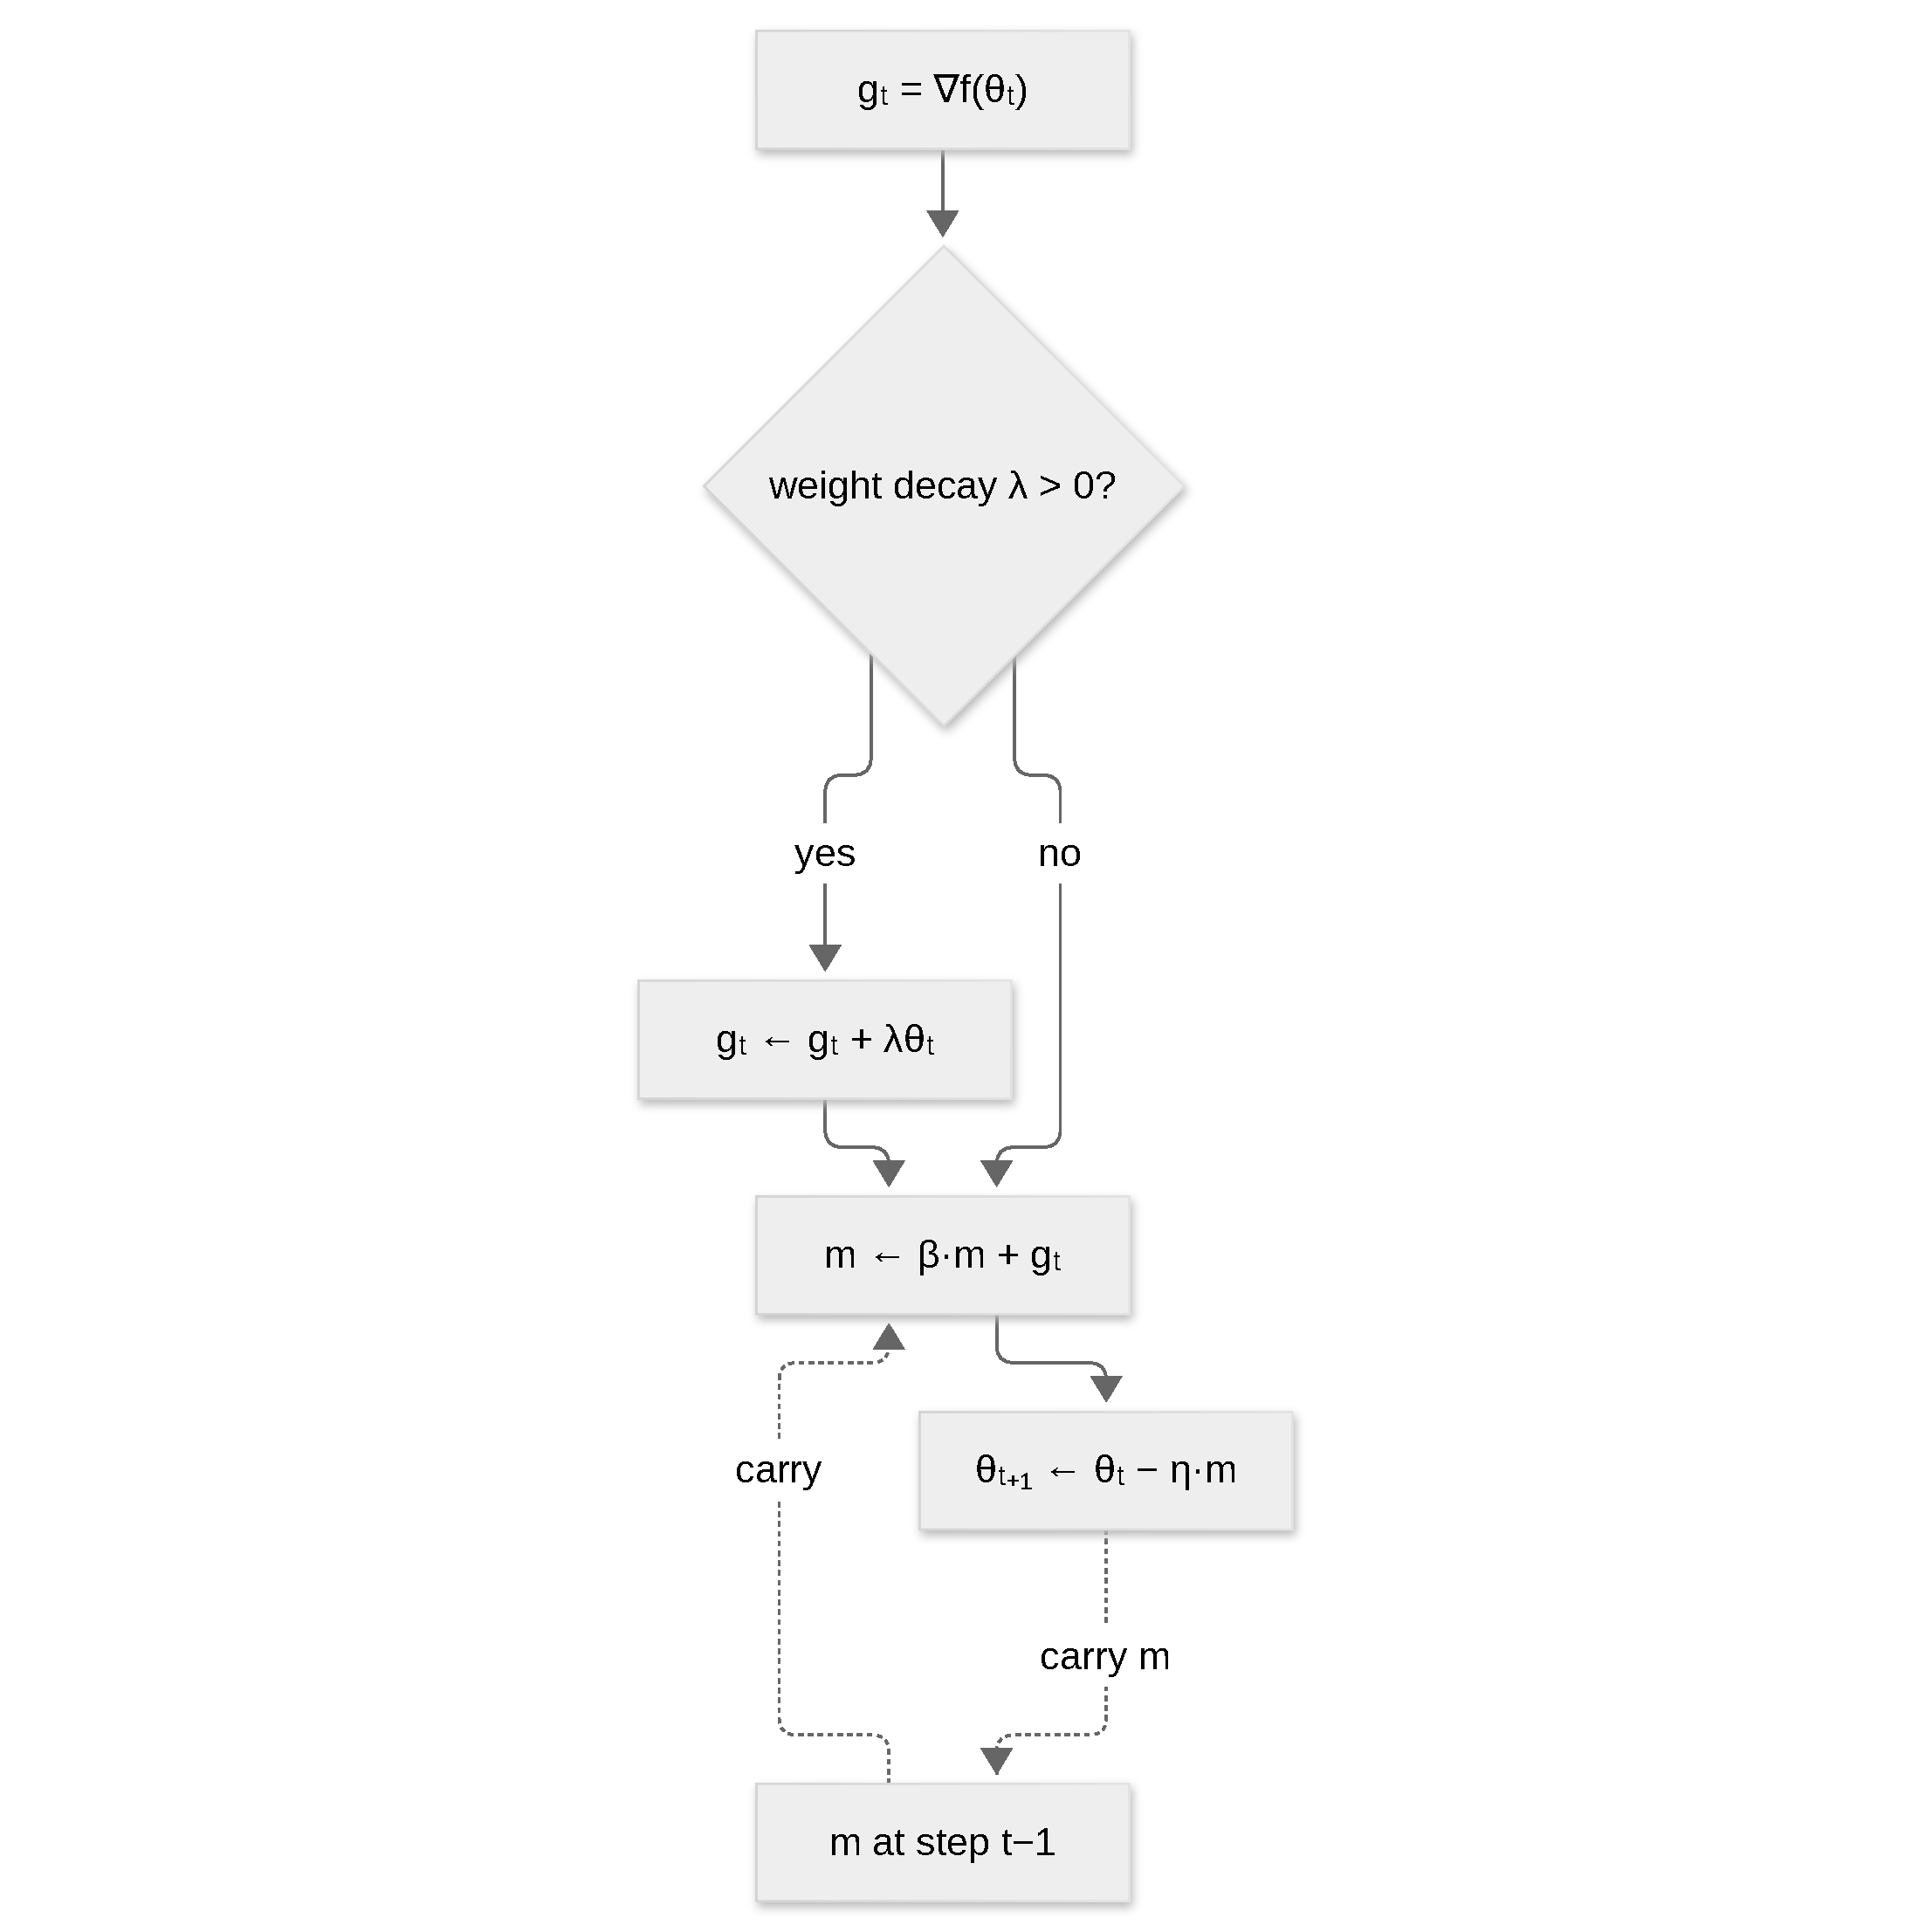
\includegraphics{../paper/figures/optimizers/sgd-momentum.pdf}}
\caption{Flujo por paso de SGD con momentum: decaimiento L2 opcional, acumulación exponencial de momentum y actualización de parámetros con paso fijo.}
\label{fig:opt-sgd-momentum}
\end{figure}
La actualización clásica acumula un búfer de momentum y luego aplica una tasa de aprendizaje fija. En cada iteración $t$, el algoritmo mantiene un promedio móvil exponencial $m_t$ de los gradientes pasados:
\begin{align}
m_t &= \beta m_{t-1} + g_t \\
\theta_{t+1} &= \theta_t - \eta m_t
\end{align}
donde $g_t = \nabla f(\theta_t)$, $\beta \in [0.8, 0.99]$ controla la decadencia del momentum y $\eta$ es la tasa de aprendizaje fija. El término de momentum actúa como velocidad: acelera el movimiento en direcciones consistentes mientras amortigua oscilaciones en direcciones variables.

\begin{algorithm}[H]
\caption{SGD con Momentum}
\label{alg:sgd-momentum}
\begin{algorithmic}[1]
\Require Parámetros iniciales $\theta_0$, tasa de aprendizaje $\eta$, coeficiente de momentum $\beta$, decadencia de peso $\lambda$
\Ensure Parámetros actualizados $\theta_T$
\State Inicializar: búfer de momentum $m \gets 0$
\For{$t = 0, 1, 2, \ldots, T-1$}
    \State Calcular gradiente: $g_t \gets \nabla f(\theta_t)$
    \If{decadencia\_de\_peso $> 0$}
        \State $g_t \gets g_t + \lambda \theta_t$ \Comment{Regularización L2}
    \EndIf
    \State Actualizar momentum: $m \gets \beta \cdot m + g_t$
    \State Actualizar parámetros: $\theta_{t+1} \gets \theta_t - \eta \cdot m$
\EndFor
\Return $\theta_T$
\end{algorithmic}
\end{algorithm}

\paragraph{Contras.}
\begin{itemize}[leftmargin=*]
\item Escasa robustez frente a la heterogeneidad de curvatura: una única tasa global no puede adaptarse a todos los grupos de parámetros.
\item Fuerte dependencia de programaciones de tasa de aprendizaje cuidadosamente diseñadas.
\end{itemize}

\paragraph{Ventajas.}
\begin{itemize}[leftmargin=*]
\item Baja sobrecarga de memoria: un único búfer de momentum por parámetro.
\item Fuerte generalización cuando se ajusta cuidadosamente, y una actualización simple de implementar.
\end{itemize}

\paragraph{Adam y AdamW.}
\begin{figure}[H]
\centering
\fitfigure{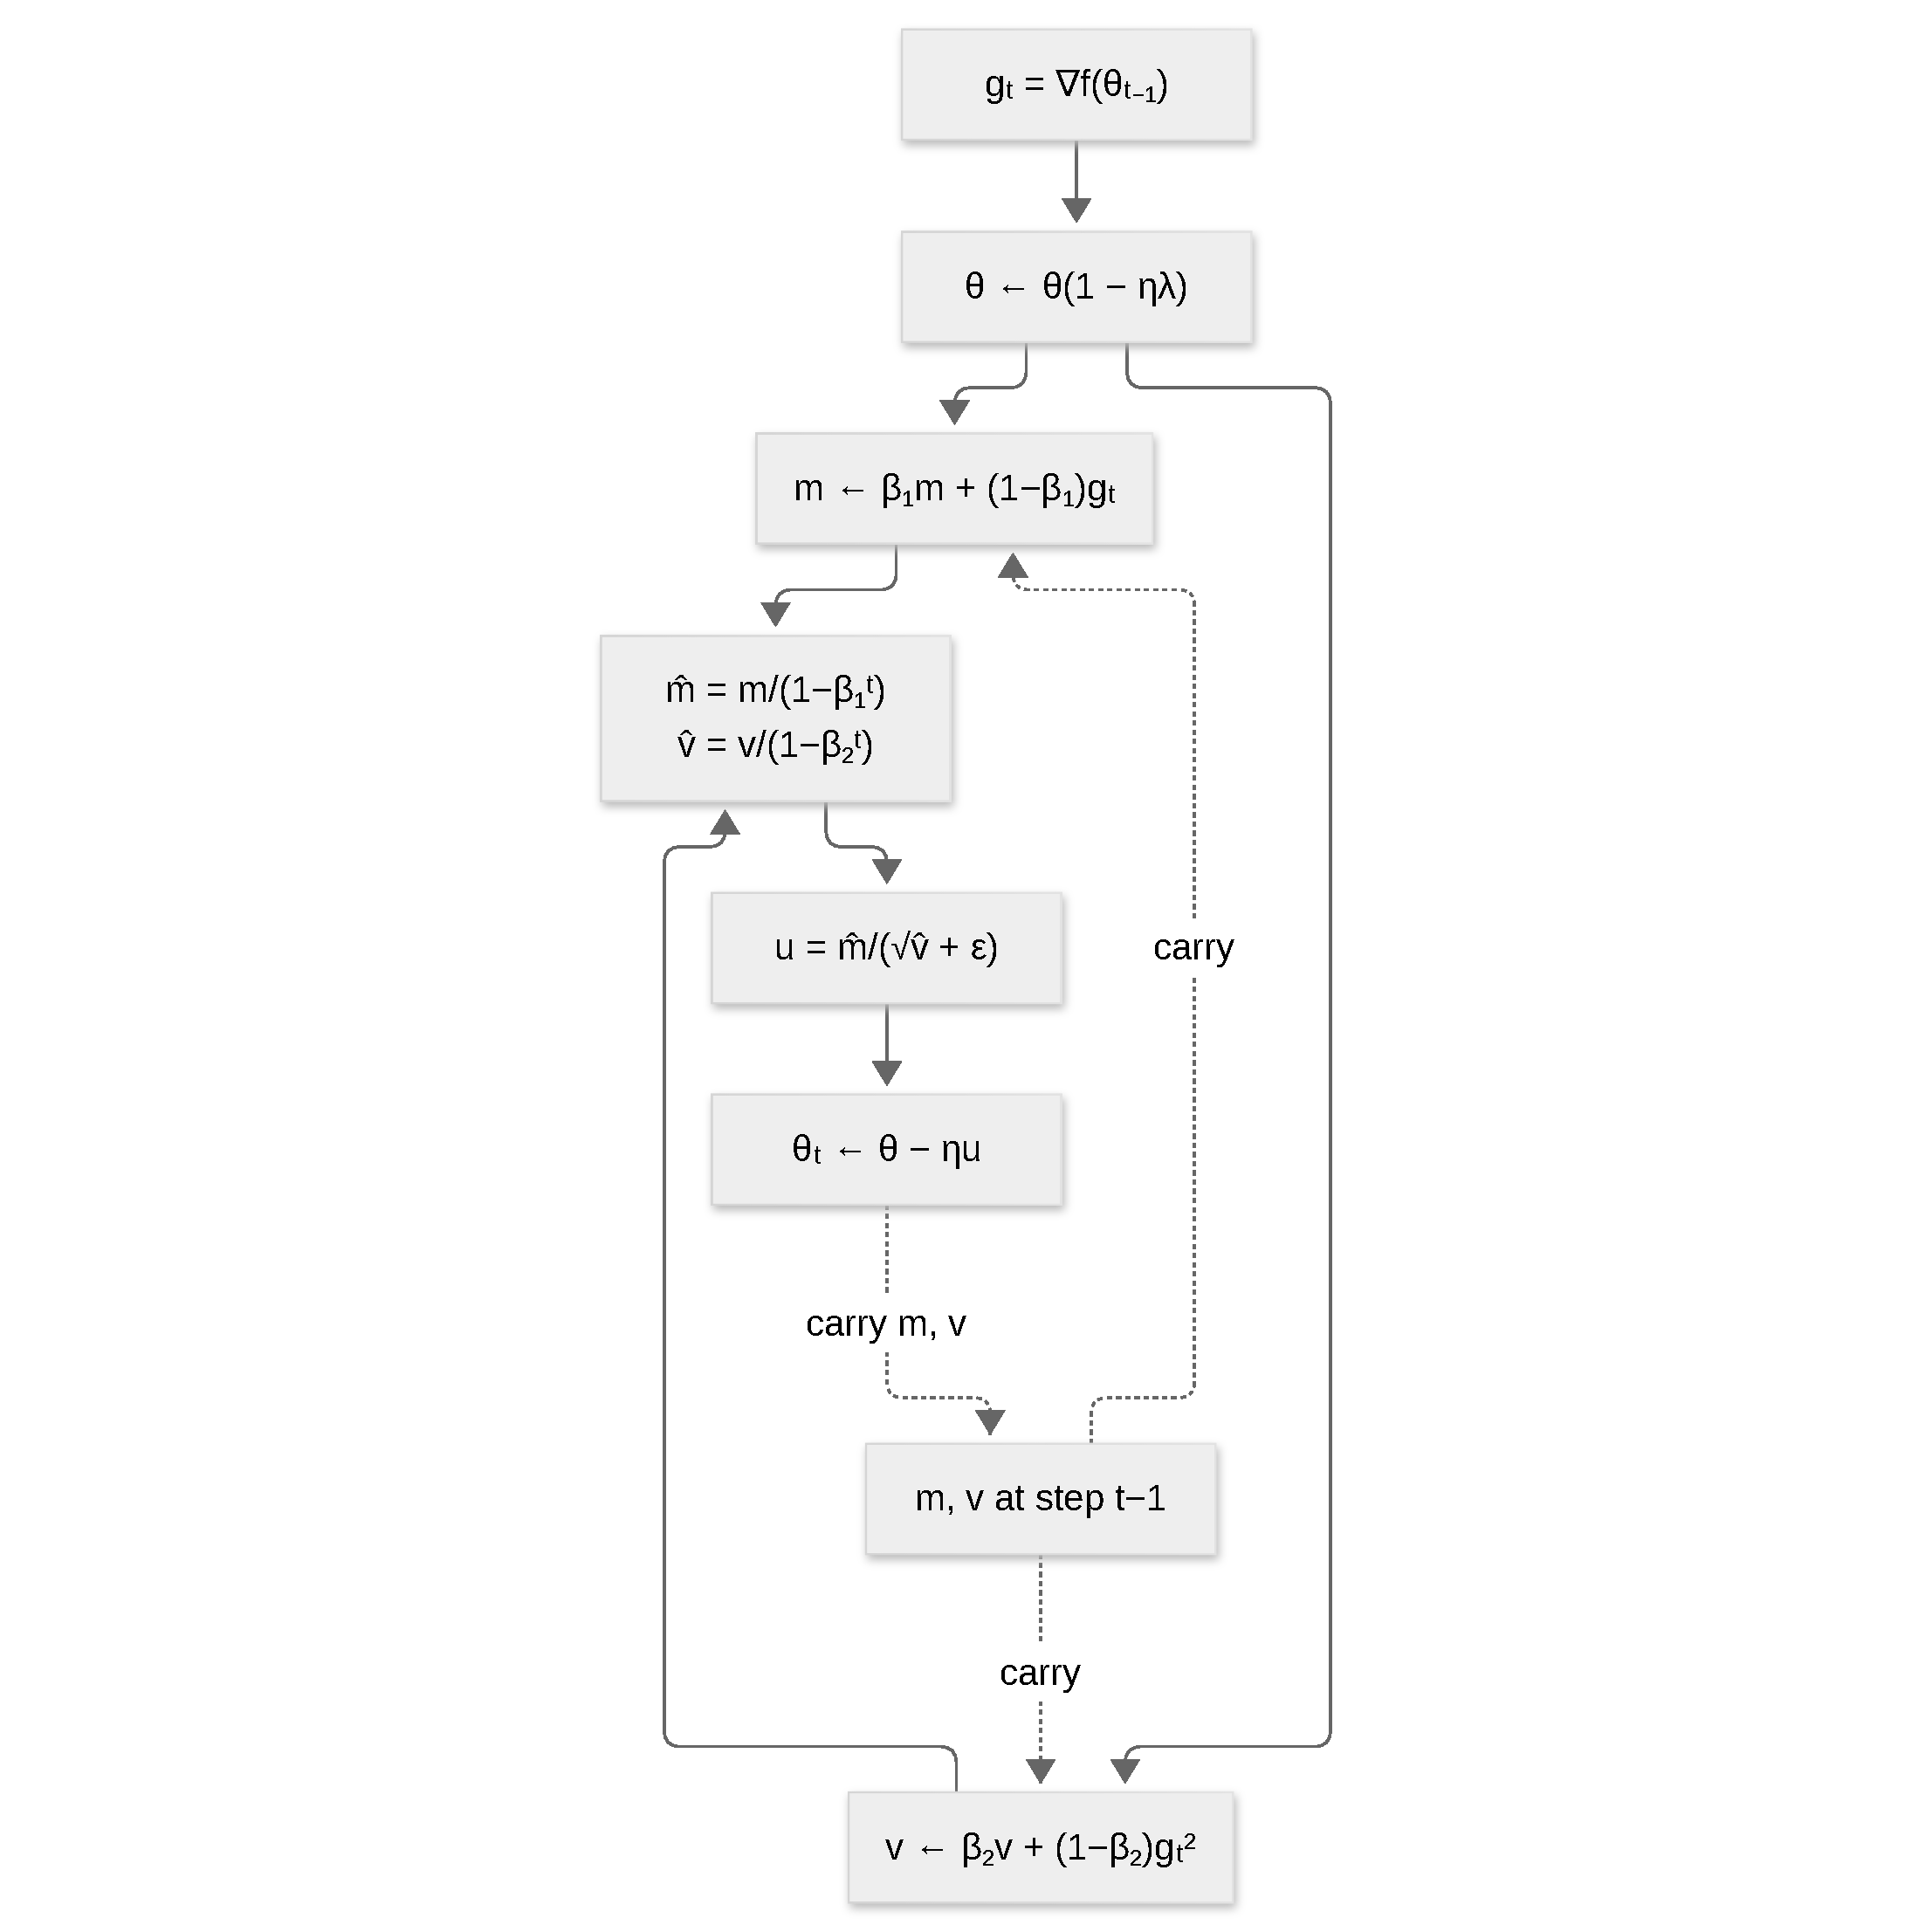
\includegraphics{../paper/figures/optimizers/adamw.pdf}}
\caption{Flujo por paso de AdamW: decaimiento de pesos desacoplado, EMAs de primer y segundo momento, corrección de sesgo y actualización adaptativa elemento a elemento.}
\label{fig:opt-adamw}
\end{figure}
Adam rastrea promedios móviles exponenciales tanto del primer momento (media) como del segundo momento (varianza no centrada) para lograr tasas de aprendizaje adaptativas elemento a elemento. La regla de actualización es:
\begin{align}
m_t &= \beta_1 m_{t-1} + (1-\beta_1) g_t \\
v_t &= \beta_2 v_{t-1} + (1-\beta_2) g_t^2 \\
\hat{m}_t &= \frac{m_t}{1-\beta_1^t}, \quad \hat{v}_t = \frac{v_t}{1-\beta_2^t} \quad \text{(corrección de sesgo)} \\
\theta_{t+1} &= \theta_t - \eta \left(\frac{\hat{m}_t}{\sqrt{\hat{v}_t}+\epsilon}\right)
\end{align}
AdamW introduce una modificación crucial: la decadencia de peso se aplica directamente a los parámetros (desacoplada de los gradientes): $\theta_t \gets \theta_t(1-\eta\lambda)$ en lugar de añadir $\lambda\theta_t$ al gradiente. Este desacoplamiento evita que el escalado adaptativo interfiera con la fuerza de la regularización.

\begin{algorithm}[H]
\caption{AdamW (Adam con Decadencia de Peso Desacoplada)}
\label{alg:adamw}
\begin{algorithmic}[1]
\Require Parámetros iniciales $\theta_0$, tasa de aprendizaje $\eta$, tasas de decadencia exponencial $\beta_1, \beta_2 \in [0,1)$
\Require Constante de momentum $\epsilon$, decadencia de peso $\lambda$
\Ensure Parámetros actualizados $\theta_T$
\State Inicializar: primer momento $m \gets 0$, segundo momento $v \gets 0$, contador de pasos $t \gets 0$
\For{$t = 1, 2, \ldots, T$}
    \State Calcular gradiente: $g_t \gets \nabla f(\theta_{t-1})$
    \State Decadencia de peso (desacoplada): $\theta_{t-1} \gets \theta_{t-1}(1 - \eta\lambda)$
    \State Actualizar momentos: $m \gets \beta_1 m + (1-\beta_1) g_t$
    \State $v \gets \beta_2 v + (1-\beta_2) g_t^2$
    \State Corrección de sesgo: $\hat{m} \gets m / (1 - \beta_1^t)$, $\hat{v} \gets v / (1 - \beta_2^t)$
    \State Actualizar parámetros: $\theta_t \gets \theta_{t-1} - \eta (\hat{m} / (\sqrt{\hat{v}} + \epsilon))$
\EndFor
\Return $\theta_T$
\end{algorithmic}
\end{algorithm}

\paragraph{Contras.}
\begin{itemize}[leftmargin=*]
\item Almacena tensores de primer y segundo momento para cada parámetro, duplicando la memoria del estado del optimizador respecto a SGD.
\item El escalado adaptativo elemento a elemento puede interferir con la regularización si el decaimiento de pesos no se desacopla.
\end{itemize}

\paragraph{Ventajas.}
\begin{itemize}[leftmargin=*]
\item Línea base práctica para el ajuste fino de transformadores: convergencia rápida y tolerancia a la variación de hiperparámetros.
\item El decaimiento de pesos desacoplado mantiene la fuerza de la regularización independiente del escalado adaptativo.
\end{itemize}

\paragraph{RAdam (Adam Rectificado).}
\begin{figure}[H]
\centering
\fitfigure{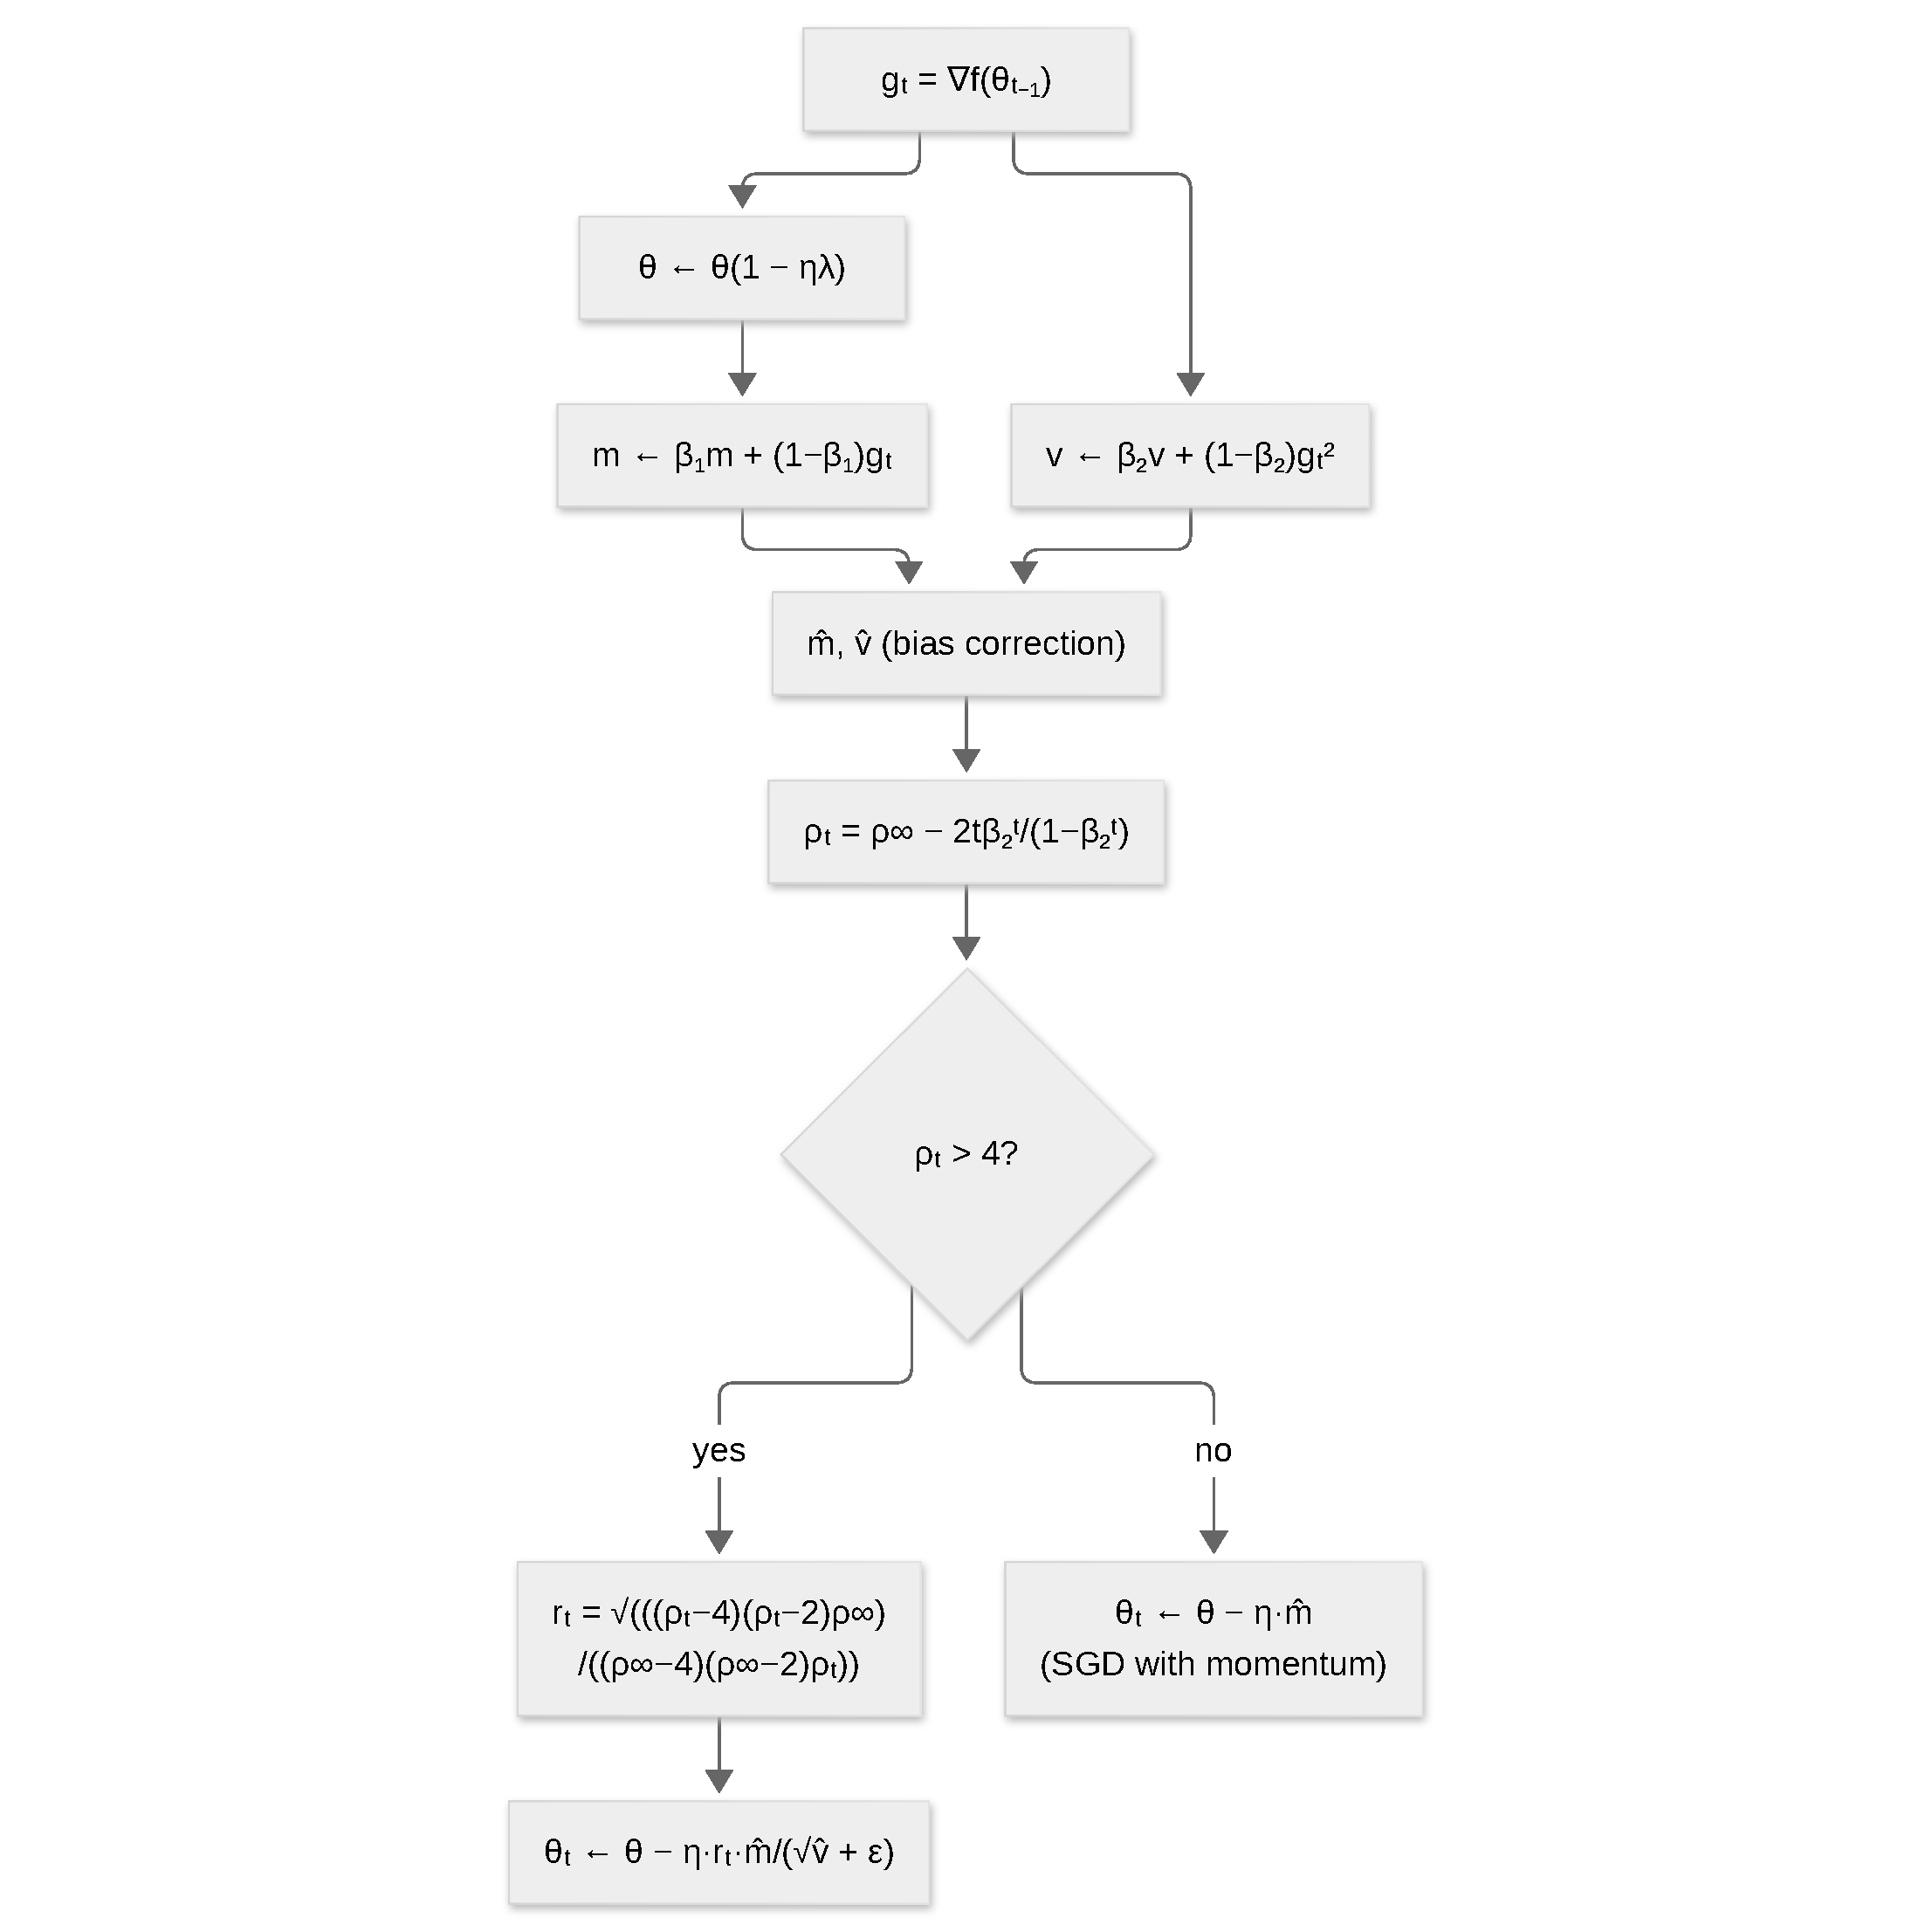
\includegraphics{../paper/figures/optimizers/radam.pdf}}
\caption{Flujo por paso de RAdam: rectificación por ventana SMA con retroceso a SGD con momentum en los primeros pasos.}
\label{fig:opt-radam}
\end{figure}
RAdam aborda la inestabilidad de Adam en el entrenamiento temprano rectificando dinámicamente la tasa de aprendizaje adaptativa. La observación clave es que el segundo momento $v_t$ tiene una varianza muy alta en los primeros pasos, causando un escalado adaptativo poco fiable. RAdam calcula la longitud efectiva de la ventana de promedio móvil simple (SMA):
\[\rho_t = \rho_{\infty} - \frac{2t\beta_2^t}{1-\beta_2^t}, \quad \text{donde} \quad \rho_{\infty} = \frac{2}{1-\beta_2}-1\]
Cuando $\rho_t > 4$ (suficientes muestras para la estimación de varianza), RAdam aplica el escalado adaptativo con un término de rectificación:
\[r_t = \sqrt{\frac{(\rho_t-4)(\rho_t-2)\rho_{\infty}}{(\rho_{\infty}-4)(\rho_{\infty}-2)\rho_t}}, \quad \theta_{t+1} = \theta_t - \eta r_t \frac{\hat{m}_t}{\sqrt{\hat{v}_t}+\epsilon}\]
Cuando $\rho_t \leq 4$, RAdam retrocede a SGD con momentum: $\theta_{t+1} = \theta_t - \eta\hat{m}_t$.

\begin{algorithm}[H]
\caption{RAdam (Adam Rectificado)}
\label{alg:radam}
\begin{algorithmic}[1]
\Require Parámetros iniciales $\theta_0$, tasa de aprendizaje $\eta$, $\beta_1, \beta_2$, decadencia de peso $\lambda$
\Ensure Parámetros actualizados $\theta_T$
\State Inicializar: $m \gets 0$, $v \gets 0$, $t \gets 0$
\State Calcular: $\rho_\infty \gets 2/(1-\beta_2) - 1$
\For{$t = 1, 2, \ldots, T$}
    \State $g_t \gets \nabla f(\theta_{t-1})$
    \If{decadencia\_de\_peso $> 0$}
        \State $\theta_{t-1} \gets \theta_{t-1}(1 - \eta\lambda)$
    \EndIf
    \State $m \gets \beta_1 m + (1-\beta_1) g_t$
    \State $v \gets \beta_2 v + (1-\beta_2) g_t^2$
    \State $\hat{m} \gets m/(1-\beta_1^t)$, $\hat{v} \gets v/(1-\beta_2^t)$
    \State $\rho_t \gets \rho_\infty - 2t \beta_2^t / (1 - \beta_2^t)$
    \If{$\rho_t > 4$}
        \State $r_t \gets \sqrt{((\rho_t-4)(\rho_t-2)\rho_\infty) / ((\rho_\infty-4)(\rho_\infty-2)\rho_t)}$
        \State $\theta_t \gets \theta_{t-1} - \eta r_t \hat{m} / (\sqrt{\hat{v}} + \epsilon)$
    \Else
        \State $\theta_t \gets \theta_{t-1} - \eta \hat{m}$ \Comment{SGD con momentum}
    \EndIf
\EndFor
\Return $\theta_T$
\end{algorithmic}
\end{algorithm}

\paragraph{Contras.}
\begin{itemize}[leftmargin=*]
\item Añade contabilidad de rectificación sobre el estado de momentos de Adam.
\item El beneficio se reduce cuando ya se usa una programación de calentamiento bien ajustada.
\end{itemize}

\paragraph{Ventajas.}
\begin{itemize}[leftmargin=*]
\item Elimina la necesidad de calentamiento manual al rectificar la tasa adaptativa.
\item Retrocede con elegancia a SGD con momentum mientras las estimaciones de varianza no son fiables, mejorando la robustez.
\end{itemize}

\subsection{Momentum Avanzado y Reducción de Varianza (2024--2025)}
\paragraph{Adan (Momentum Nesterov Adaptativo).}
\begin{figure}[H]
\centering
\fitfigure{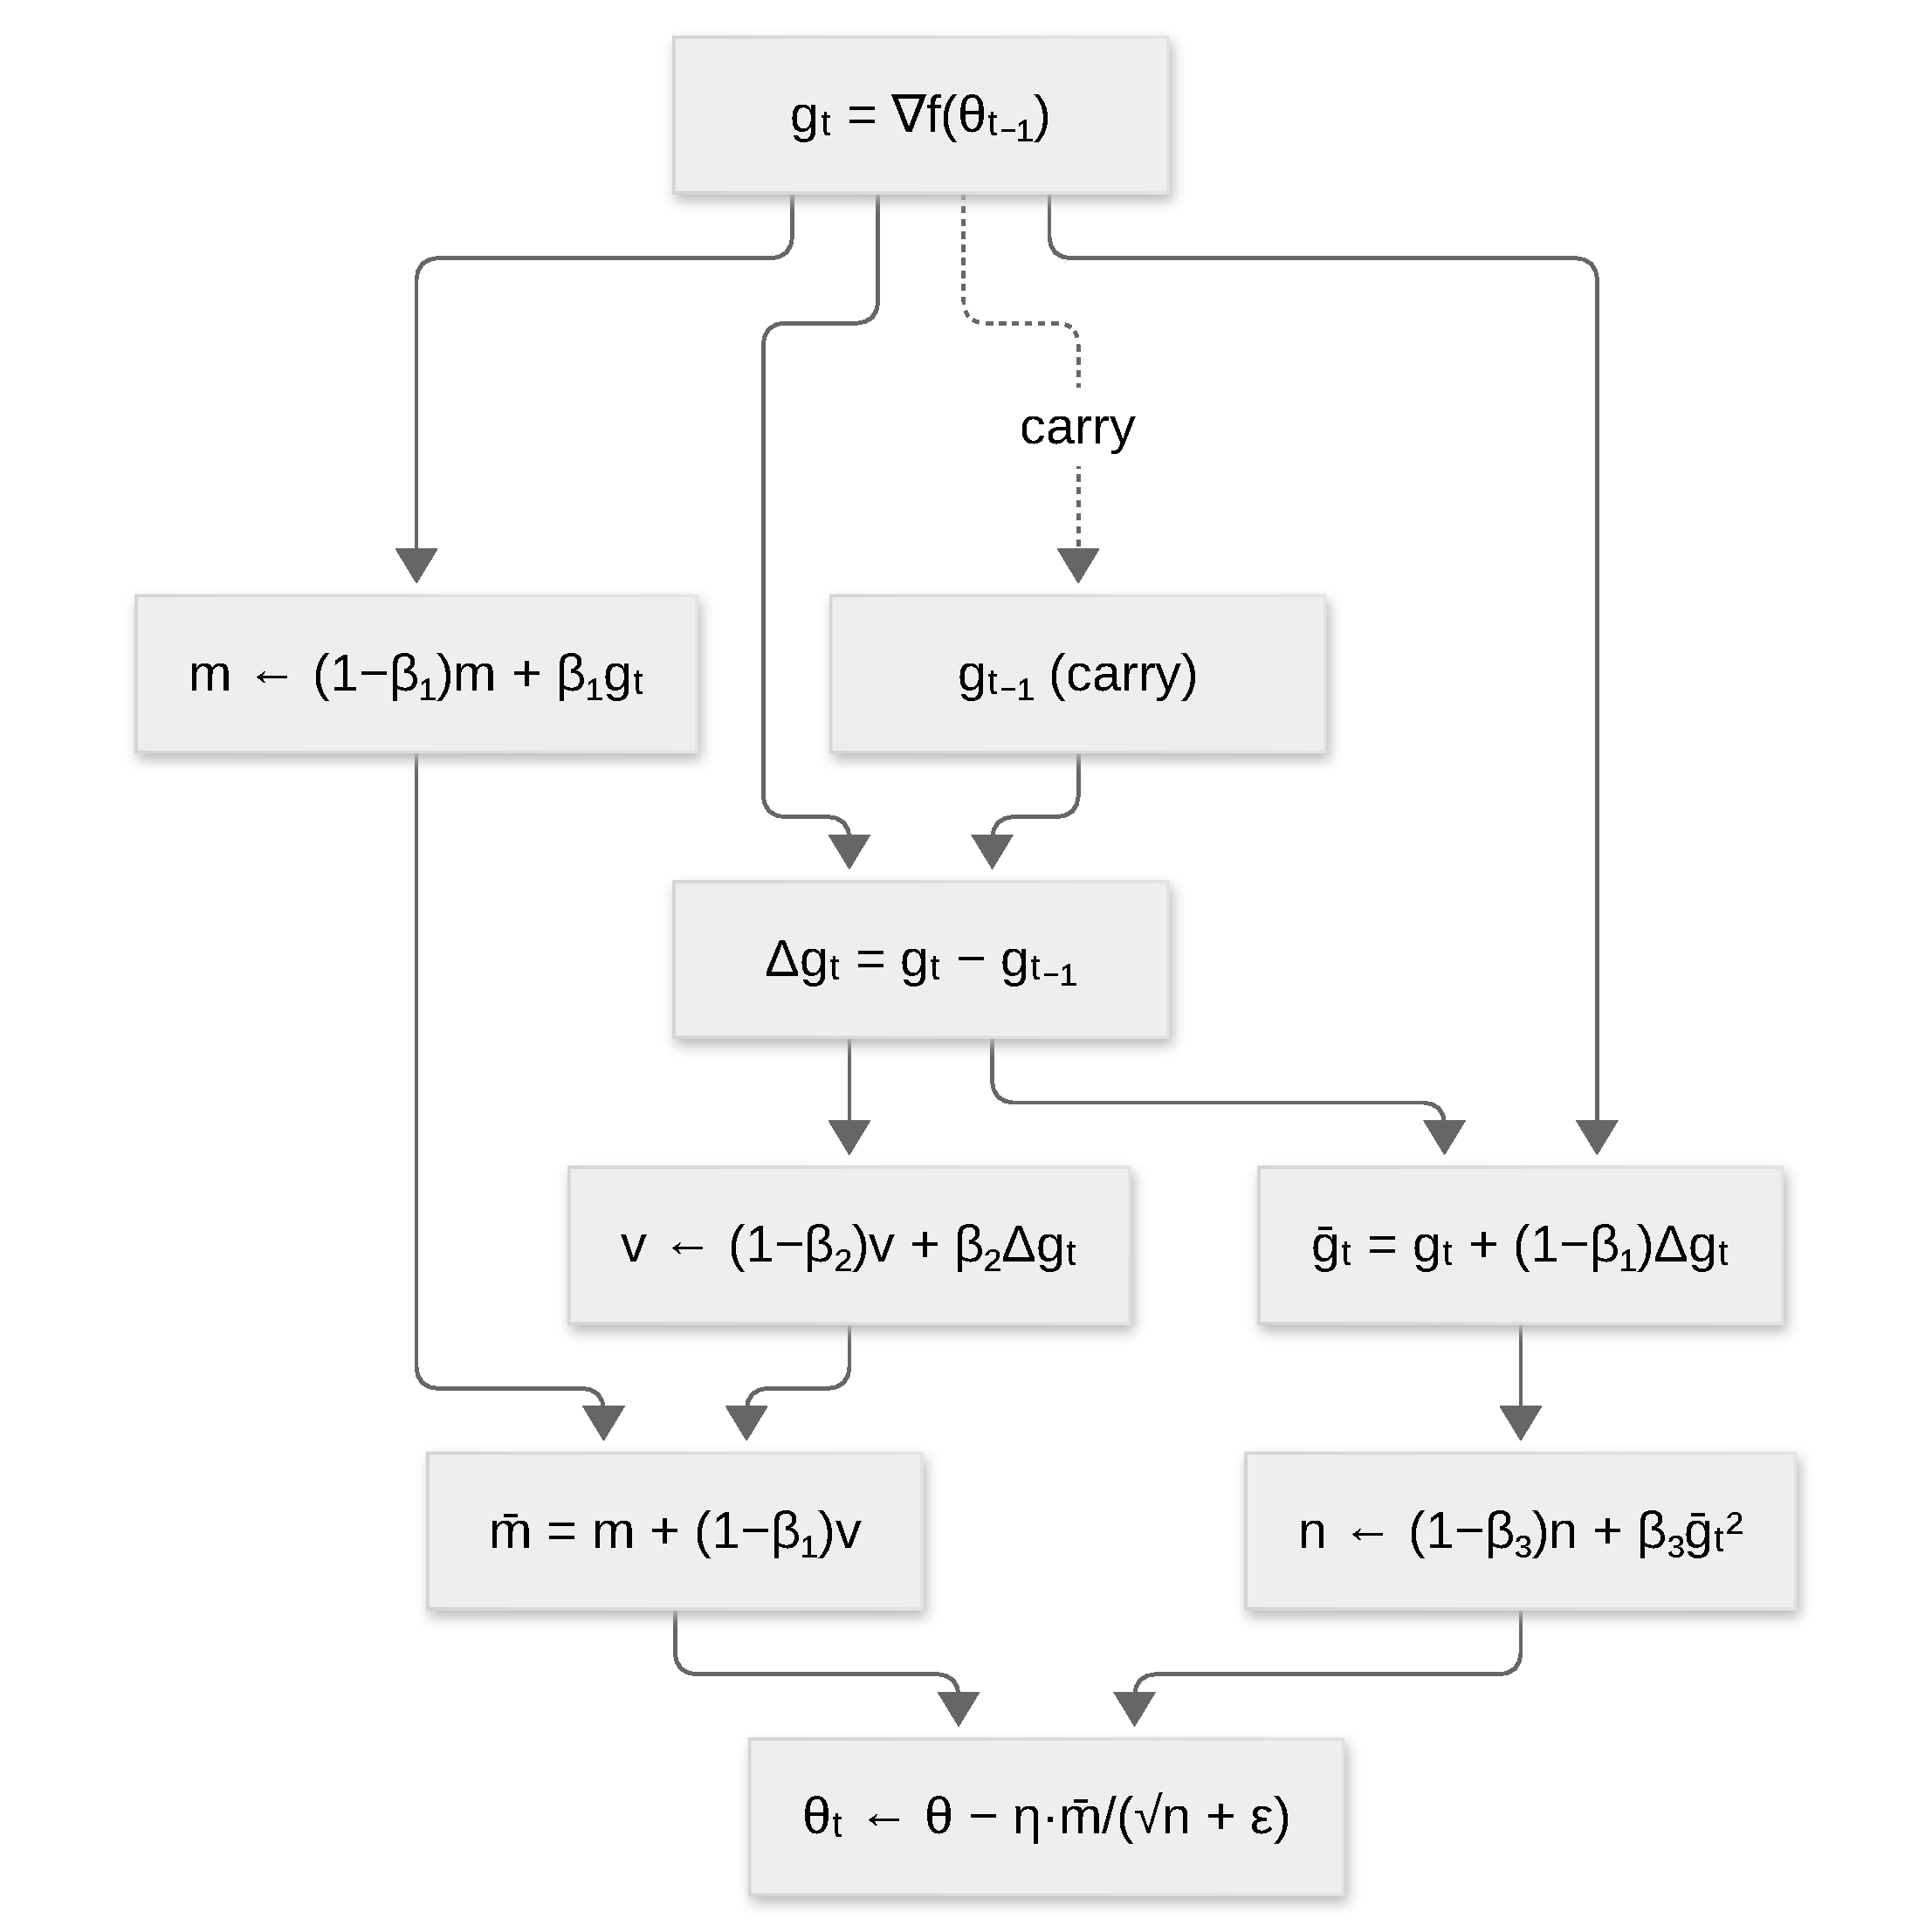
\includegraphics{../paper/figures/optimizers/adan.pdf}}
\caption{Flujo por paso de Adan: estimación de momentum de Nesterov a partir de la diferencia de gradientes, con tres búferes de estado y un paso de momentum combinado.}
\label{fig:opt-adan}
\end{figure}
Adan reformula la aceleración de Nesterov sin el cálculo de gradiente adicional requerido por el SGD Nesterov clásico. El algoritmo mantiene tres búferes de momentum:
\begin{align}
m_t &= (1-\beta_1)m_{t-1} + \beta_1 g_t \quad\text{(primer momento)} \\
v_t &= (1-\beta_2)v_{t-1} + \beta_2(g_t - g_{t-1}) \quad\text{(velocidad/diferencia de gradientes)} \\
n_t &= (1-\beta_3)n_{t-1} + \beta_3[g_t + (1-\beta_1)(g_t-g_{t-1})]^2 \quad\text{(segundo momento Nesterov)}
\end{align}
El término de \textbf{Estimación de Momentum Nesterov} (NME) $\bar{g}_t = g_t + (1-\beta_1)(g_t-g_{t-1})$ estima el gradiente en una posición futura sin evaluarlo. La actualización combina el momentum con la velocidad:
\[\bar{m}_t = m_t + (1-\beta_1)v_t, \quad \theta_{t+1} = \theta_t - \eta\frac{\bar{m}_t}{\sqrt{n_t}+\epsilon}\]

\begin{algorithm}[H]
\caption{Adan (Momentum Nesterov Adaptativo)}
\label{alg:adan}
\begin{algorithmic}[1]
\Require Parámetros iniciales $\theta_0$, tasa de aprendizaje $\eta$, $\beta_1, \beta_2, \beta_3 \in (0,1)$
\Ensure Parámetros actualizados $\theta_T$
\State Inicializar: $m \gets 0$, $v \gets 0$, $n \gets 0$, $g_{-1} \gets 0$ (gradiente anterior)
\For{$t = 1, 2, \ldots, T$}
    \State $g_t \gets \nabla f(\theta_{t-1})$
    \State $m \gets (1-\beta_1) m + \beta_1 g_t$
    \State $\Delta g_t \gets g_t - g_{t-1}$
    \State $v \gets (1-\beta_2) v + \beta_2 \Delta g_t$
    \State Estimación Nesterov: $\bar{g}_t \gets g_t + (1-\beta_1) \Delta g_t$
    \State $n \gets (1-\beta_3) n + \beta_3 \bar{g}_t^2$
    \State Momentum combinado: $\bar{m} \gets m + (1-\beta_1) v$
    \State $\theta_t \gets \theta_{t-1} - \eta (\bar{m} / (\sqrt{n} + \epsilon))$
    \State $g_{t-1} \gets g_t$
\EndFor
\Return $\theta_T$
\end{algorithmic}
\end{algorithm}

\paragraph{Contras.}
\begin{itemize}[leftmargin=*]
\item Tres búferes tipo momentum aumentan la sobrecarga de memoria respecto a Adam.
\item Contabilidad adicional de la diferencia de gradientes en cada paso.
\end{itemize}

\paragraph{Ventajas.}
\begin{itemize}[leftmargin=*]
\item Aceleración estilo Nesterov sin una evaluación adicional del gradiente.
\item Convergencia rápida en arquitecturas diversas (CNN, GAN, transformadores).
\end{itemize}

\paragraph{ADOPT (Adam con Ajuste Óptimo Podado).}
\begin{figure}[H]
\centering
\fitfigure{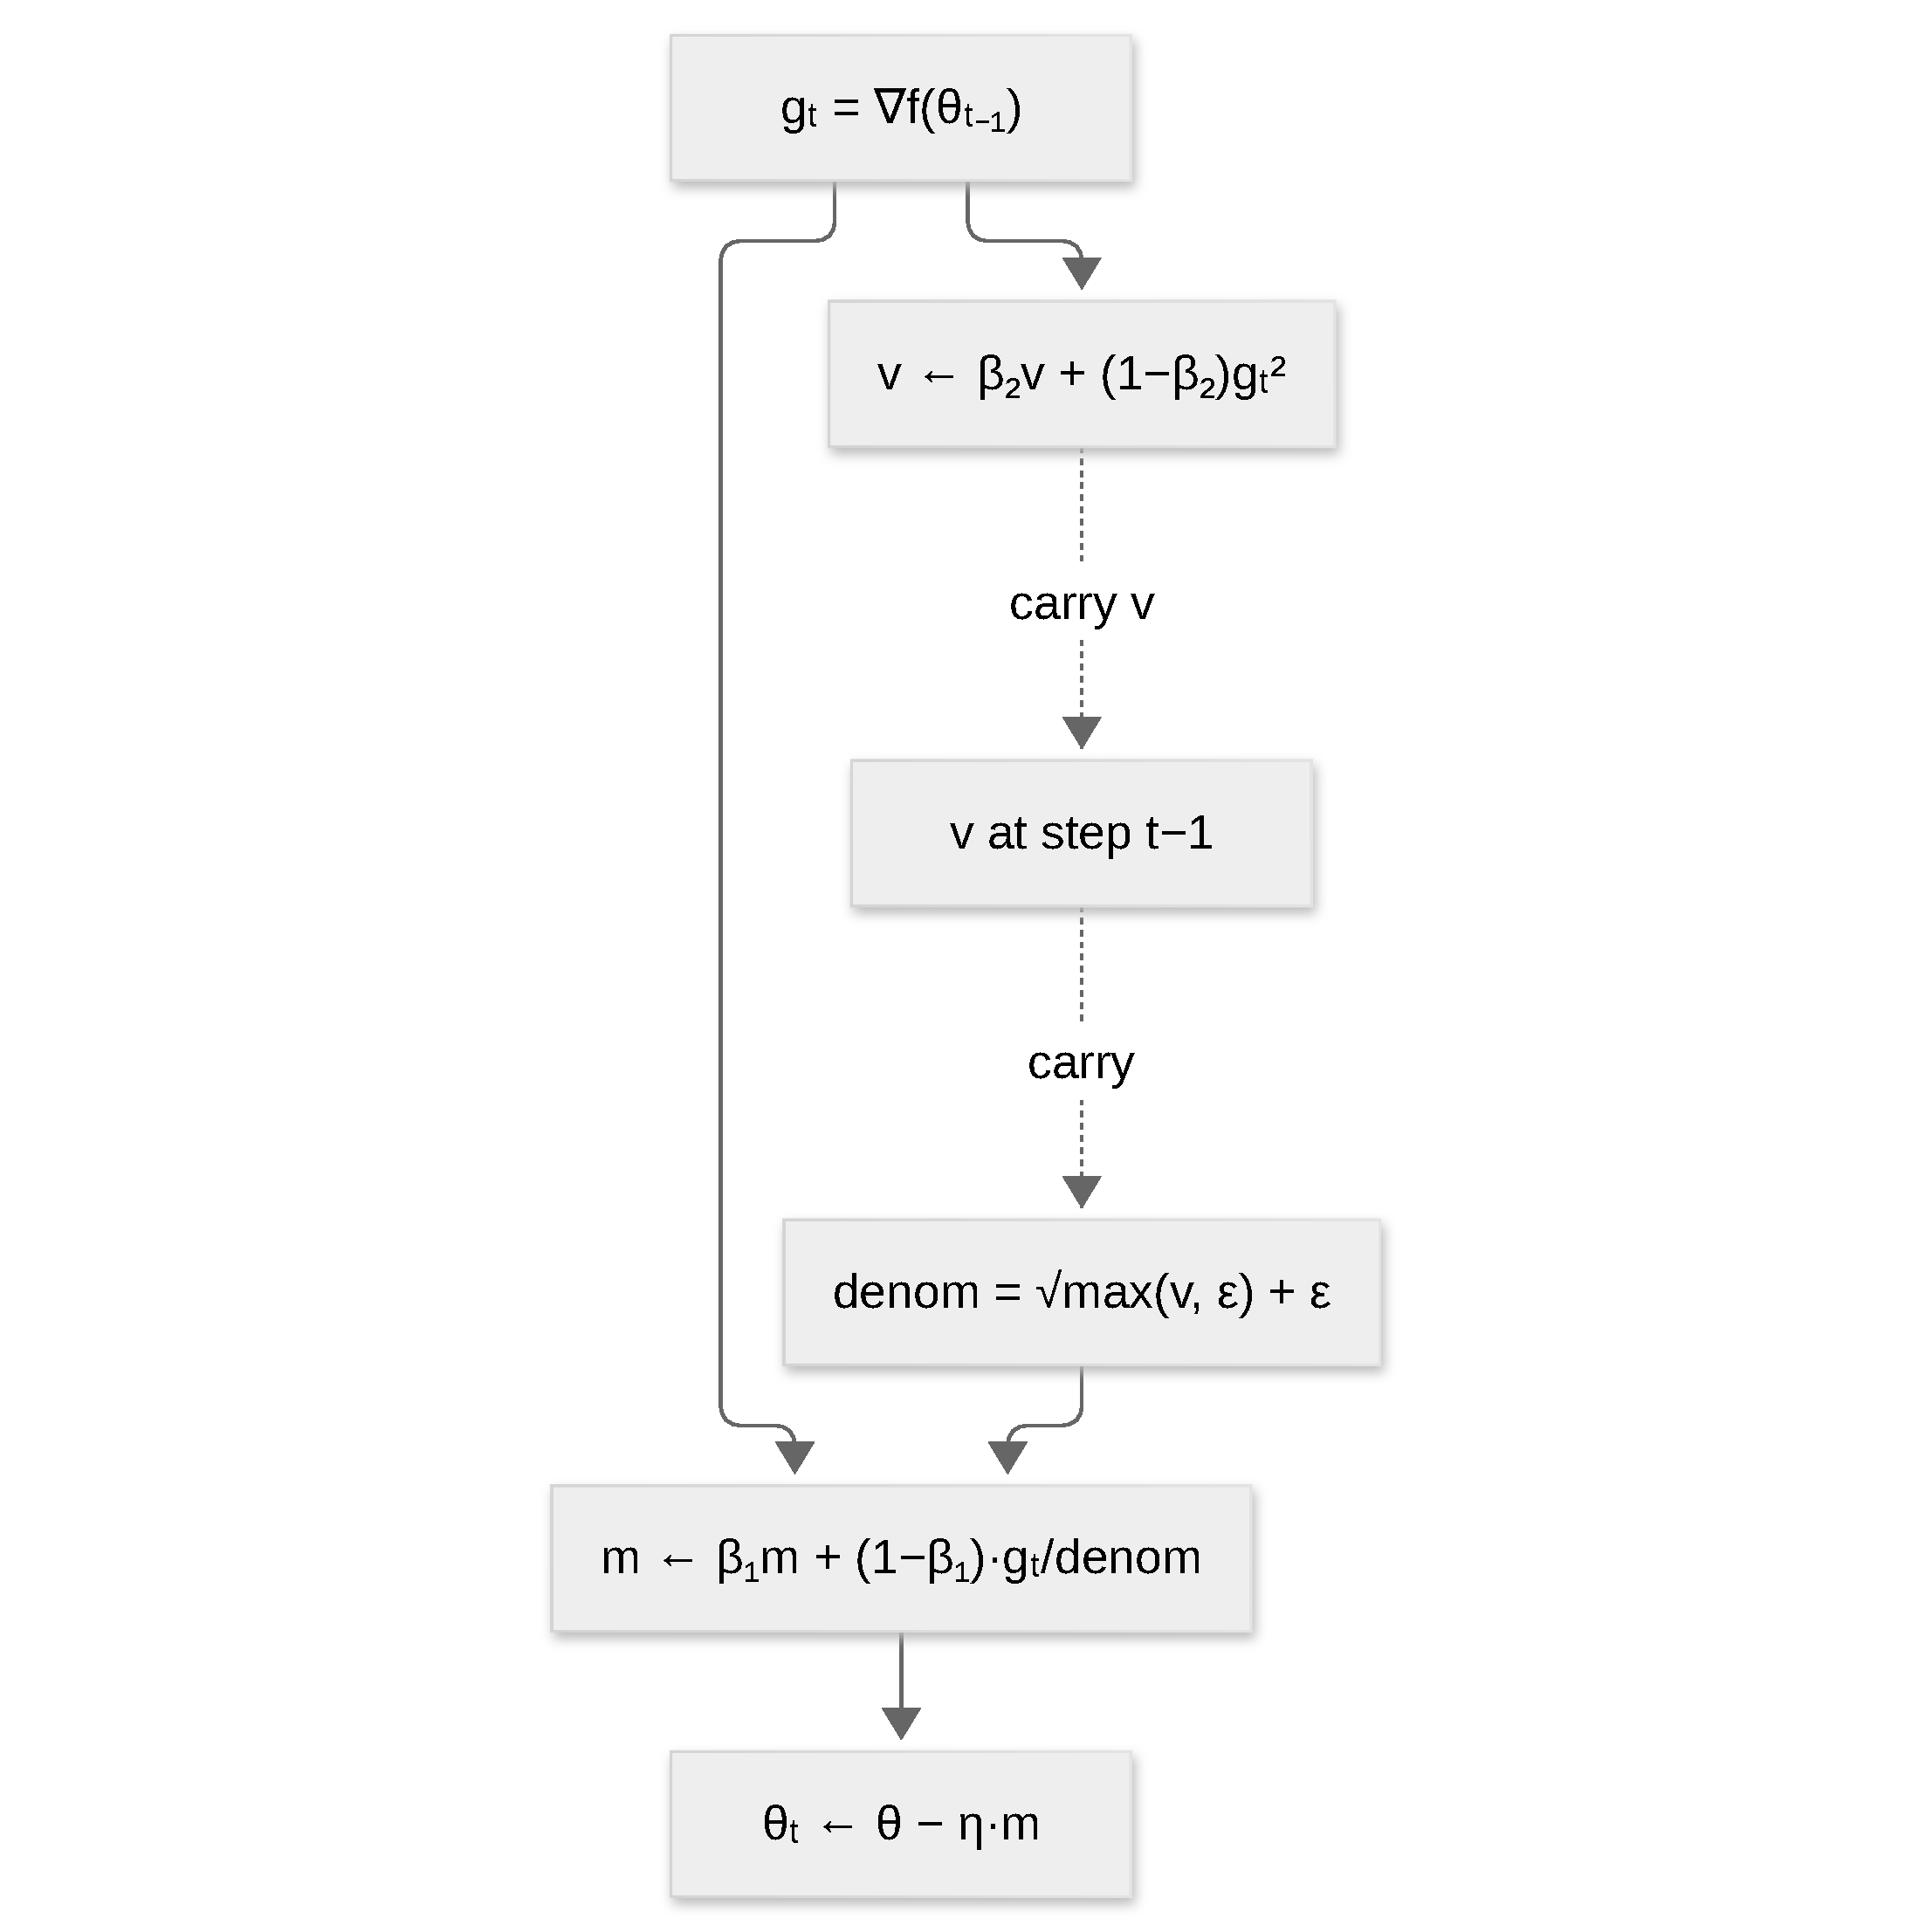
\includegraphics{../paper/figures/optimizers/adopt.pdf}}
\caption{Flujo por paso de ADOPT: el segundo momento del paso anterior normaliza el gradiente actual antes de actualizar el primer momento.}
\label{fig:opt-adopt}
\end{figure}
ADOPT corrige un problema teórico fundamental en Adam: el gradiente aparece tanto en la estimación del primer momento como en la del segundo momento, creando circularidad. ADOPT \textbf{desacopla} utilizando el segundo momento del paso anterior para el denominador:
\begin{align}
v_t &= \beta_2 v_{t-1} + (1-\beta_2)g_t^2 \\
m_t &= \beta_1 m_{t-1} + (1-\beta_1)\frac{g_t}{\sqrt{v_{t-1}}+\epsilon} \quad\text{(usa $v_{t-1}$, no $v_t$)} \\
\theta_{t+1} &= \theta_t - \eta m_t
\end{align}

\begin{algorithm}[H]
\caption{ADOPT (Adam con Ajuste Óptimo Podado)}
\label{alg:adopt}
\begin{algorithmic}[1]
\Require Parámetros iniciales $\theta_0$, tasa de aprendizaje $\eta$, $\beta_1, \beta_2$, tolerancia $\epsilon$
\Ensure Parámetros actualizados $\theta_T$
\State Inicializar: $m \gets 0$, $v \gets 0$
\For{$t = 1, 2, \ldots, T$}
    \State $g_t \gets \nabla f(\theta_{t-1})$
    \If{decadencia\_de\_peso $> 0$}
        \State $\theta_{t-1} \gets \theta_{t-1}(1 - \eta\lambda)$
    \EndIf
    \State Usar segundo momento \textbf{anterior}: $\text{denom} \gets \sqrt{\max(v, \epsilon)} + \epsilon$
    \State Actualizar primer momento usando varianza anterior: $m \gets \beta_1 m + (1-\beta_1)(g_t / \text{denom})$
    \State Actualizar segundo momento con gradiente \textbf{actual}: $v \gets \beta_2 v + (1-\beta_2) g_t^2$
    \State $\theta_t \gets \theta_{t-1} - \eta m$
\EndFor
\Return $\theta_T$
\end{algorithmic}
\end{algorithm}

\paragraph{Contras.}
\begin{itemize}[leftmargin=*]
\item Requiere conservar el segundo momento anterior como denominador explícito.
\item Las ganancias empíricas dependen de la arquitectura y del ajuste.
\end{itemize}

\paragraph{Ventajas.}
\begin{itemize}[leftmargin=*]
\item Elimina la circularidad del gradiente de Adam y alcanza la tasa óptima $O(1/\sqrt{T})$ con \textbf{cualquier} $\beta_2 \in (0,1)$, sin suposiciones de ruido acotado.
\item Reemplazo directo de Adam con rendimiento empírico comparable o superior en visión, PLN, RL y modelado generativo.
\end{itemize}

\paragraph{AdEMAMix (Mezcla de Promedios Móviles Exponenciales).}
\begin{figure}[H]
\centering
\fitfigure{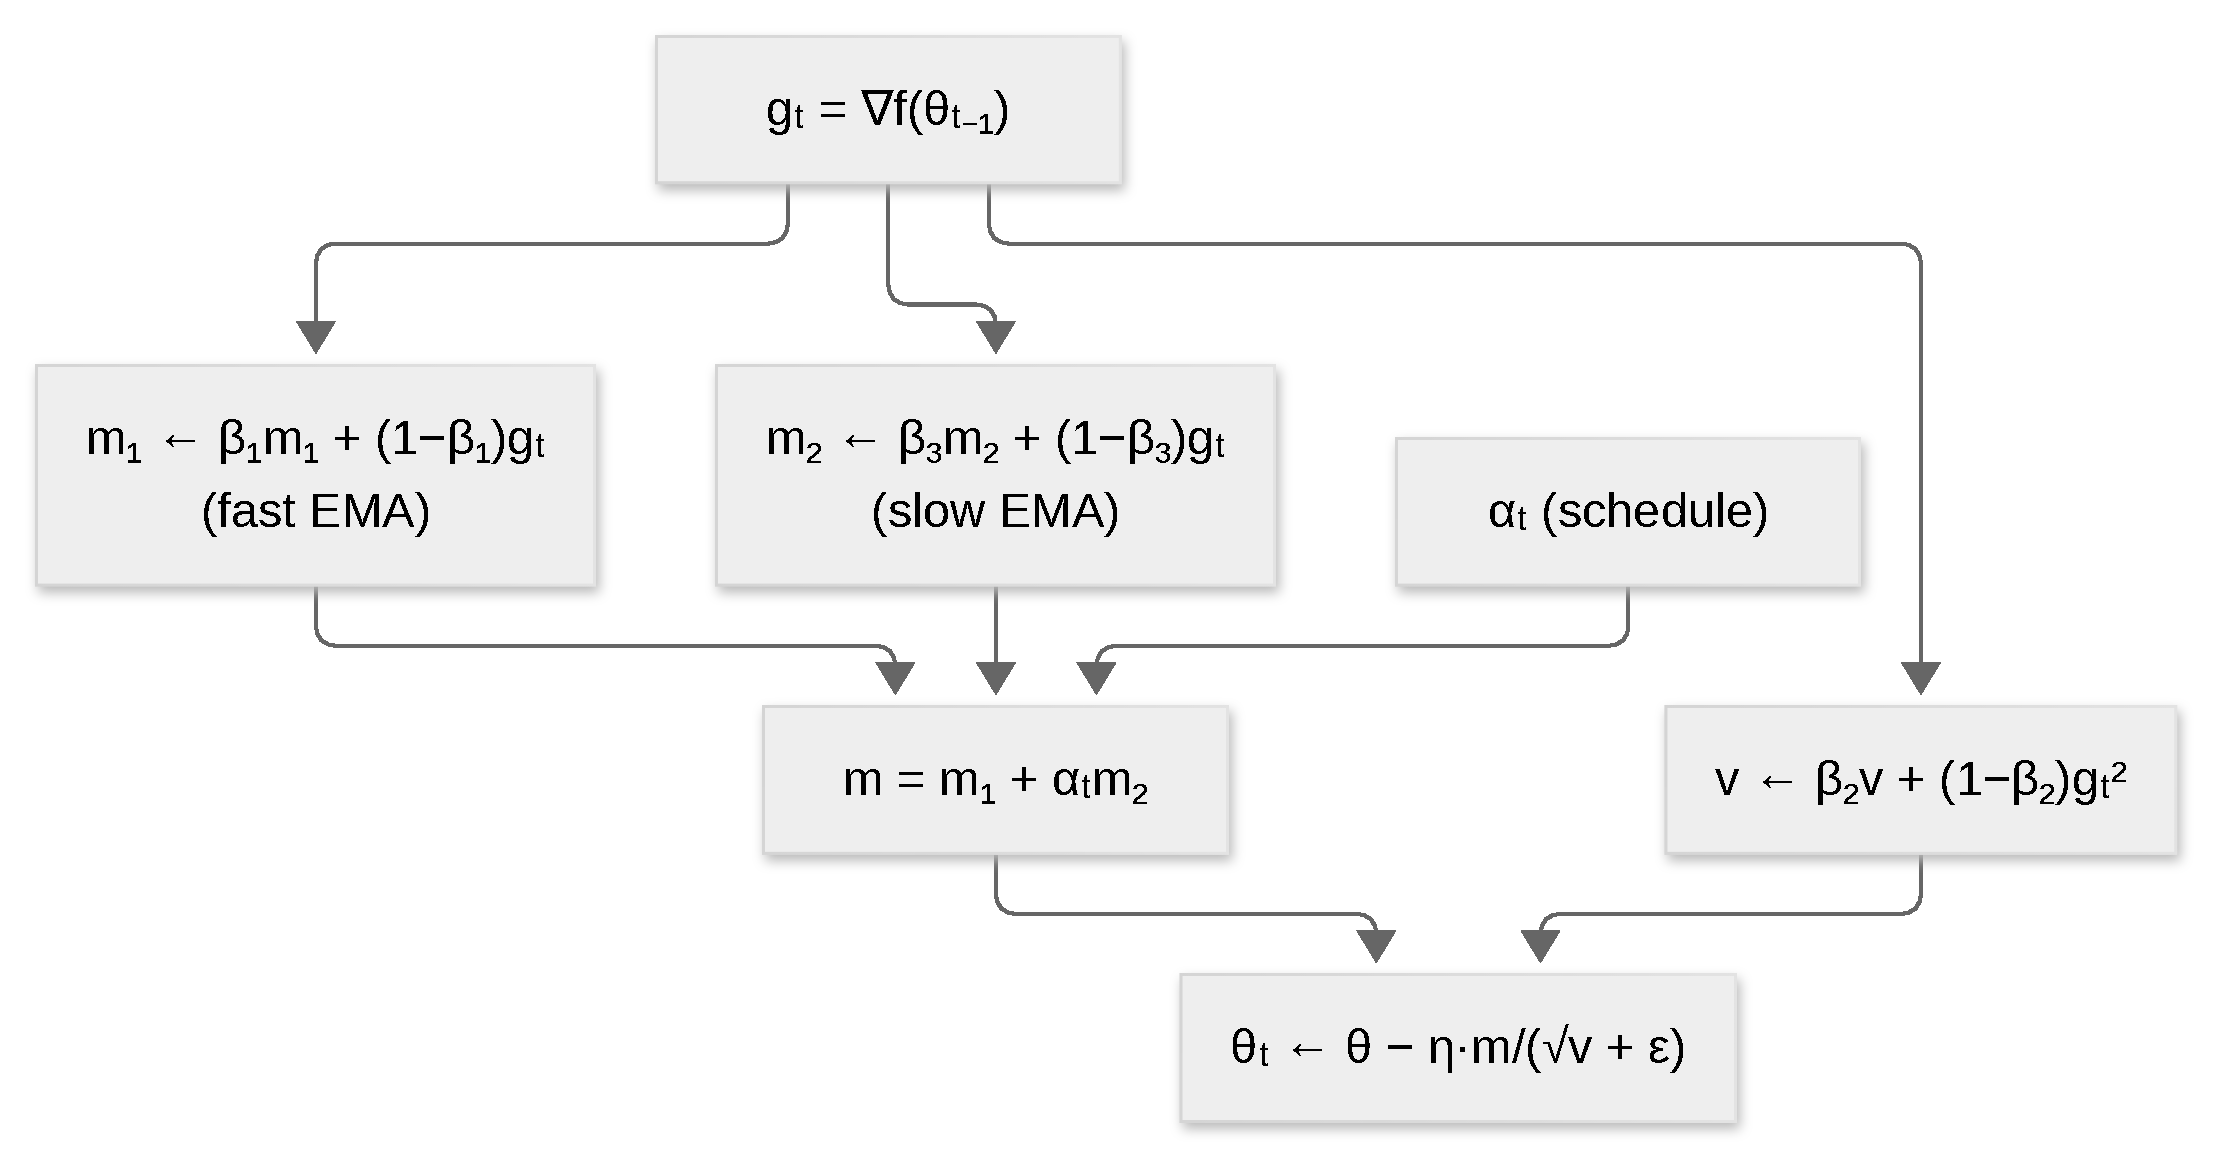
\includegraphics{../paper/figures/optimizers/ademamix.pdf}}
\caption{Flujo por paso de AdEMAMix: EMAs rápida y lenta en paralelo, mezcladas con un peso programado $\alpha_t$ antes de la actualización adaptativa.}
\label{fig:opt-ademamix}
\end{figure}
AdEMAMix reemplaza el EMA único de gradientes de Adam por una \textbf{mezcla de dos EMA}: uno de decadencia rápida y otro de decadencia lenta. Esto aborda la observación de que los gradientes siguen siendo informativos durante decenas de miles de pasos, no solo cientos:
\begin{align}
m_{1,t} &= \beta_1 m_{1,t-1} + (1-\beta_1)g_t \quad\text{(EMA rápido, $\beta_1 \approx 0.9$)} \\
m_{2,t} &= \beta_3 m_{2,t-1} + (1-\beta_3)g_t \quad\text{(EMA lento, $\beta_3 \approx 0.9999$)} \\
v_t &= \beta_2 v_{t-1} + (1-\beta_2)g_t^2 \\
m_t &= m_{1,t} + \alpha_t m_{2,t} \quad\text{(mezcla con peso programado $\alpha_t$)} \\
\theta_{t+1} &= \theta_t - \eta\frac{m_t}{\sqrt{v_t}+\epsilon}
\end{align}
El peso de la mezcla $\alpha_t$ típicamente aumenta durante el entrenamiento, permitiendo que el EMA rápido proporcione adaptación inmediata mientras que el EMA lento acumula correlaciones de gradiente a largo plazo.

\begin{algorithm}[H]
\caption{AdEMAMix (Mezcla de Promedios Móviles Exponenciales)}
\label{alg:ademamix}
\begin{algorithmic}[1]
\Require Parámetros iniciales $\theta_0$, tasa de aprendizaje $\eta$, $\beta_1$ (rápido), $\beta_3$ (lento), $\beta_2$ (segundo momento)
\Require Peso de mezcla $\alpha_t$ (típicamente creciente), tolerancia $\epsilon$
\Ensure Parámetros actualizados $\theta_T$
\State Inicializar: $m_1 \gets 0$ (EMA rápido), $m_2 \gets 0$ (EMA lento), $v \gets 0$
\For{$t = 1, 2, \ldots, T$}
    \State $g_t \gets \nabla f(\theta_{t-1})$
    \If{decadencia\_de\_peso $> 0$}
        \State $\theta_{t-1} \gets \theta_{t-1}(1 - \eta\lambda)$
    \EndIf
    \State $m_1 \gets \beta_1 m_1 + (1-\beta_1) g_t$ \Comment{EMA rápido}
    \State $m_2 \gets \beta_3 m_2 + (1-\beta_3) g_t$ \Comment{EMA lento}
    \State $v \gets \beta_2 v + (1-\beta_2) g_t^2$
    \State $m_t \gets m_1 + \alpha_t m_2$ \Comment{Mezcla}
    \State $\theta_t \gets \theta_{t-1} - \eta (m_t / (\sqrt{v} + \epsilon))$
\EndFor
\Return $\theta_T$
\end{algorithmic}
\end{algorithm}

\paragraph{Contras.}
\begin{itemize}[leftmargin=*]
\item Dos EMA de gradiente más el segundo momento casi triplican el estado del optimizador de Adam.
\item La programación de mezcla $\alpha_t$ añade un hiperparámetro que ajustar.
\end{itemize}

\paragraph{Ventajas.}
\begin{itemize}[leftmargin=*]
\item Explota información de gradiente que sigue siendo informativa durante decenas de miles de pasos.
\item Un modelo de 1.3B en 101B tokens iguala a AdamW en 197B tokens (ganancia del 95\% en eficiencia de datos), lo que sugiere menor olvido.
\end{itemize}

\paragraph{MARS (Haciendo Brillar las Tasas de Aprendizaje Adaptativas).}
\begin{figure}[H]
\centering
\fitfigure{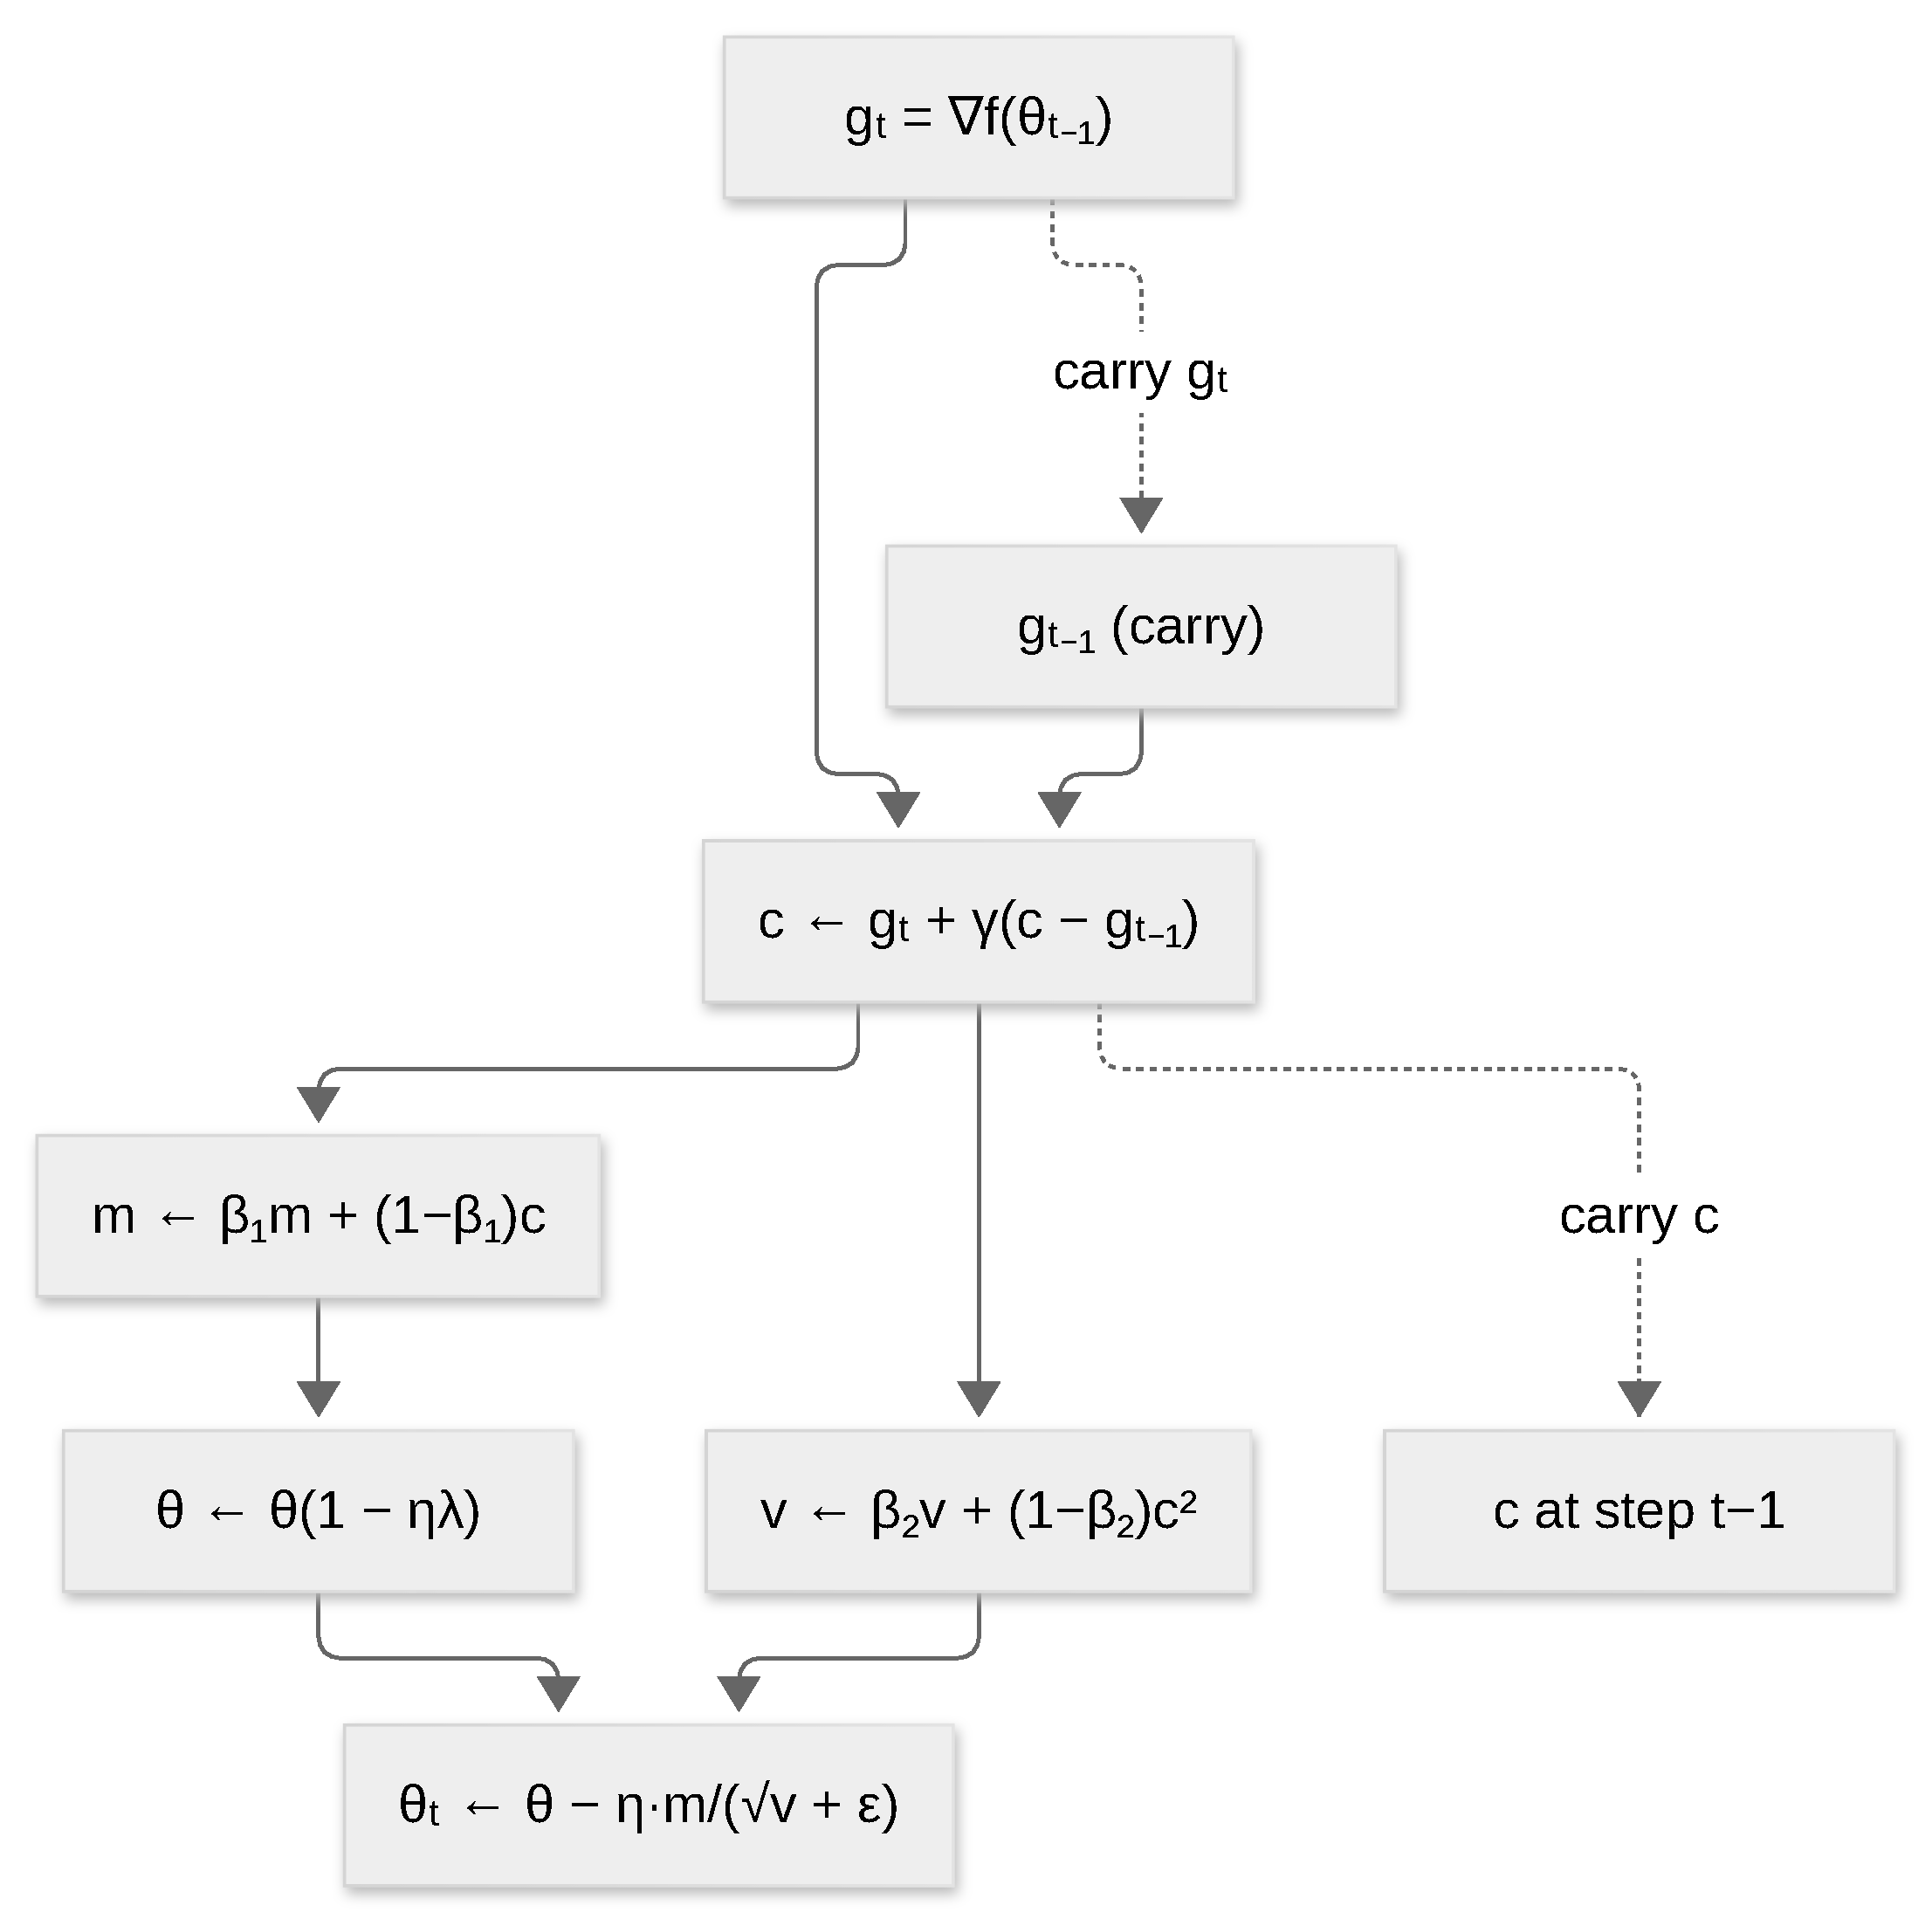
\includegraphics{../paper/figures/optimizers/mars.pdf}}
\caption{Flujo por paso de MARS: una estimación recursiva de gradiente con varianza reducida que alimenta los momentos de primer y segundo orden estilo Adam.}
\label{fig:opt-mars}
\end{figure}
MARS combina métodos de gradiente precondicionado (ej., AdamW) con \textbf{reducción de varianza} mediante momentum recursivo estocástico escalado. La innovación central es una estimación del gradiente con varianza reducida:
\begin{align}
c_t &= g_t + \gamma(c_{t-1} - g_{t-1}) \quad\text{(estimación recursiva tipo SVRG)} \\
m_t &= \beta_1 m_{t-1} + (1-\beta_1)c_t \\
v_t &= \beta_2 v_{t-1} + (1-\beta_2)c_t^2 \\
\theta_{t+1} &= \theta_t - \eta\frac{m_t}{\sqrt{v_t}+\epsilon}
\end{align}
donde $\gamma \in [0.01, 0.1]$ controla cuánta información de gradiente histórico se retiene. El gradiente con varianza reducida $c_t$ actúa como un filtro de ruido implícito, amplificando las direcciones de señal consistentes y amortiguando el ruido contradictorio.

\begin{algorithm}[H]
\caption{MARS (Haciendo Brillar las Tasas de Aprendizaje Adaptativas)}
\label{alg:mars}
\begin{algorithmic}[1]
\Require Parámetros iniciales $\theta_0$, tasa de aprendizaje $\eta$, $\beta_1, \beta_2$, decadencia de peso $\lambda$
\Require Coeficiente de reducción de varianza $\gamma \in [0.01, 0.1]$
\Ensure Parámetros actualizados $\theta_T$
\State Inicializar: $m \gets 0$, $v \gets 0$, $c \gets 0$ (gradiente con varianza reducida), $g_{-1} \gets 0$
\For{$t = 1, 2, \ldots, T$}
    \State $g_t \gets \nabla f(\theta_{t-1})$
    \State Reducción de varianza: $c \gets g_t + \gamma(c - g_{t-1})$
    \State $m \gets \beta_1 m + (1-\beta_1) c$
    \State $v \gets \beta_2 v + (1-\beta_2) c^2$
    \If{decadencia\_de\_peso $> 0$}
        \State $\theta_{t-1} \gets \theta_{t-1}(1 - \eta\lambda)$
    \EndIf
    \State $\theta_t \gets \theta_{t-1} - \eta (m / (\sqrt{v} + \epsilon))$
    \State $g_{t-1} \gets g_t$
\EndFor
\Return $\theta_T$
\end{algorithmic}
\end{algorithm}

\paragraph{Contras.}
\begin{itemize}[leftmargin=*]
\item Almacena el gradiente con varianza reducida y el gradiente anterior además de los momentos de Adam.
\item El coeficiente de reducción de varianza $\gamma \in [0.01, 0.1]$ debe ajustarse.
\end{itemize}

\paragraph{Ventajas.}
\begin{itemize}[leftmargin=*]
\item Actúa como un filtro de ruido implícito, amplificando direcciones consistentes y amortiguando el ruido contradictorio.
\item MARS-AdamW supera consistentemente a AdamW por márgenes significativos en el preentrenamiento de GPT-2.
\end{itemize}

\paragraph{Optimizadores Cautelosos (Cautious AdamW, Cautious Lion).}
\begin{figure}[H]
\centering
\fitfigure{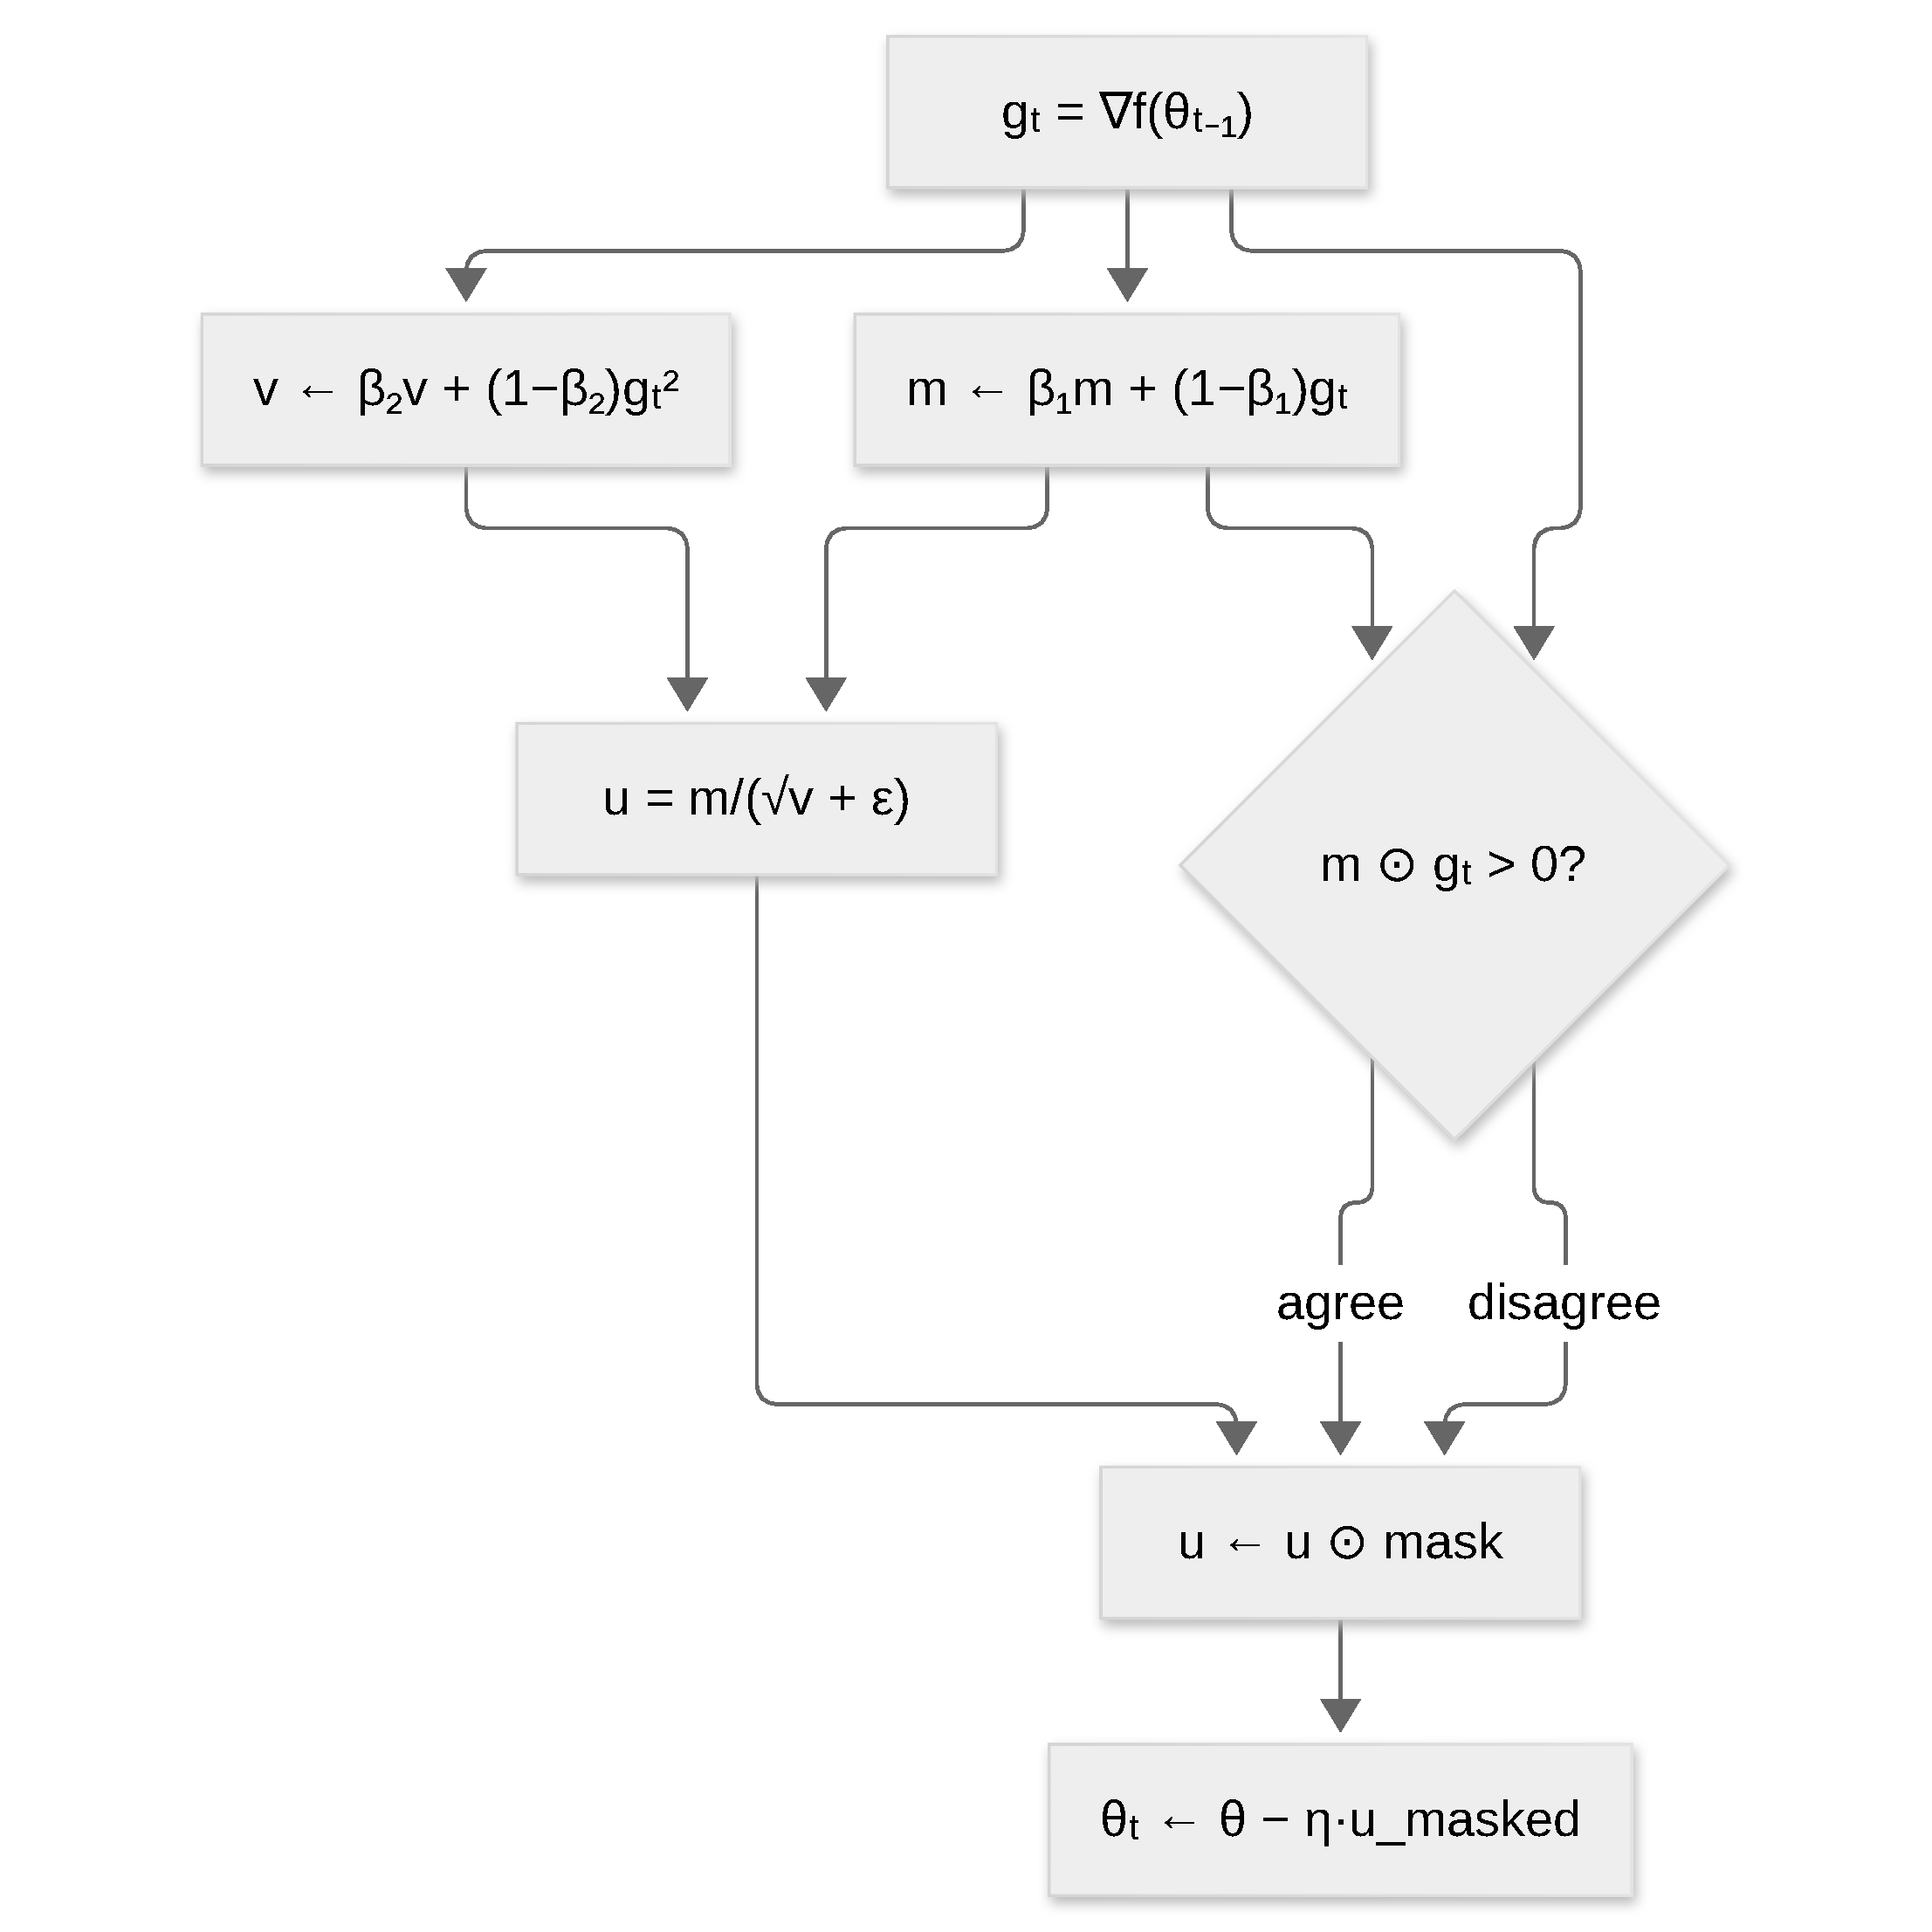
\includegraphics{../paper/figures/optimizers/cautious.pdf}}
\caption{Flujo por paso de Cautious AdamW: una máscara de consenso conserva solo las coordenadas donde momentum y gradiente coinciden.}
\label{fig:opt-cautious}
\end{figure}
El marco Cauteloso aplica una \textbf{modificación de una línea} a cualquier optimizador basado en momentum: enmascarar la actualización de modo que solo se apliquen las dimensiones donde el momentum y la dirección del gradiente coinciden:
\begin{align}
\text{mask}_i &= \begin{cases} 1 & \text{si } m_t[i] \cdot g_t[i] > 0 \quad\text{(acuerdo)} \\ 0 & \text{en caso contrario} \end{cases} \\
u_t &= \left(\frac{m_t}{\sqrt{v_t}+\epsilon}\right) \odot \text{mask} \quad\text{(enmascaramiento elemento a elemento)} \\
\theta_{t+1} &= \theta_t - \eta u_t
\end{align}
La intuición: el momentum $m_t$ estima la dirección del gradiente a partir del historial; el gradiente actual $g_t$ es la señal instantánea. Cuando ambos coinciden, el optimizador está seguro y debe actualizar agresivamente. Cuando discrepan, el optimizador está en conflicto---la tendencia histórica apunta hacia una región que pudo haber sido buena antes, pero la evidencia actual la contradice. Al enmascarar las dimensiones en conflicto, Cauteloso se vuelve más conservador y evita pasos corruptos.

\begin{algorithm}[H]
\caption{Cautious AdamW (Enmascaramiento de Actualización por Consenso)}
\label{alg:cautious}
\begin{algorithmic}[1]
\Require Parámetros iniciales $\theta_0$, tasa de aprendizaje $\eta$, $\beta_1, \beta_2$, decadencia de peso $\lambda$
\Ensure Parámetros actualizados $\theta_T$
\State Inicializar: $m \gets 0$, $v \gets 0$
\For{$t = 1, 2, \ldots, T$}
    \State $g_t \gets \nabla f(\theta_{t-1})$
    \State $m \gets \beta_1 m + (1-\beta_1) g_t$
    \State $v \gets \beta_2 v + (1-\beta_2) g_t^2$
    \State Máscara de consenso: $\text{mask}_i \gets 1$ si $m[i] \cdot g_t[i] > 0$, si no $0$ \Comment{Acuerdo}
    \State Actualización base Adam: $u \gets m / (\sqrt{v} + \epsilon)$
    \State Aplicar máscara: $u_{\text{masked}} \gets u \odot \text{mask}$ \Comment{Elemento a elemento}
    \If{decadencia\_de\_peso $> 0$}
        \State $\theta_{t-1} \gets \theta_{t-1}(1 - \eta\lambda)$
    \EndIf
    \State $\theta_t \gets \theta_{t-1} - \eta u_{\text{masked}}$
\EndFor
\Return $\theta_T$
\end{algorithmic}
\end{algorithm}

\paragraph{Contras.}
\begin{itemize}[leftmargin=*]
\item El enmascaramiento puede descartar actualizaciones útiles cuando momentum y gradiente discrepan temporalmente.
\item Requiere un optimizador base con momentum además de la máscara elemento a elemento.
\end{itemize}

\paragraph{Ventajas.}
\begin{itemize}[leftmargin=*]
\item Modificación de una línea aplicable a cualquier optimizador basado en momentum.
\item Hasta \textbf{1.47$\times$ de aceleración} en el preentrenamiento de Llama y MAE preservando las garantías de convergencia.
\end{itemize}

\subsection{Optimizadores de Lote Grande, Eficientes en Memoria y Sin Tasa de Aprendizaje}
\paragraph{LAMB (Layer-wise Adaptive Moments optimizer for Batch training).}
\begin{figure}[H]
\centering
\fitfigure{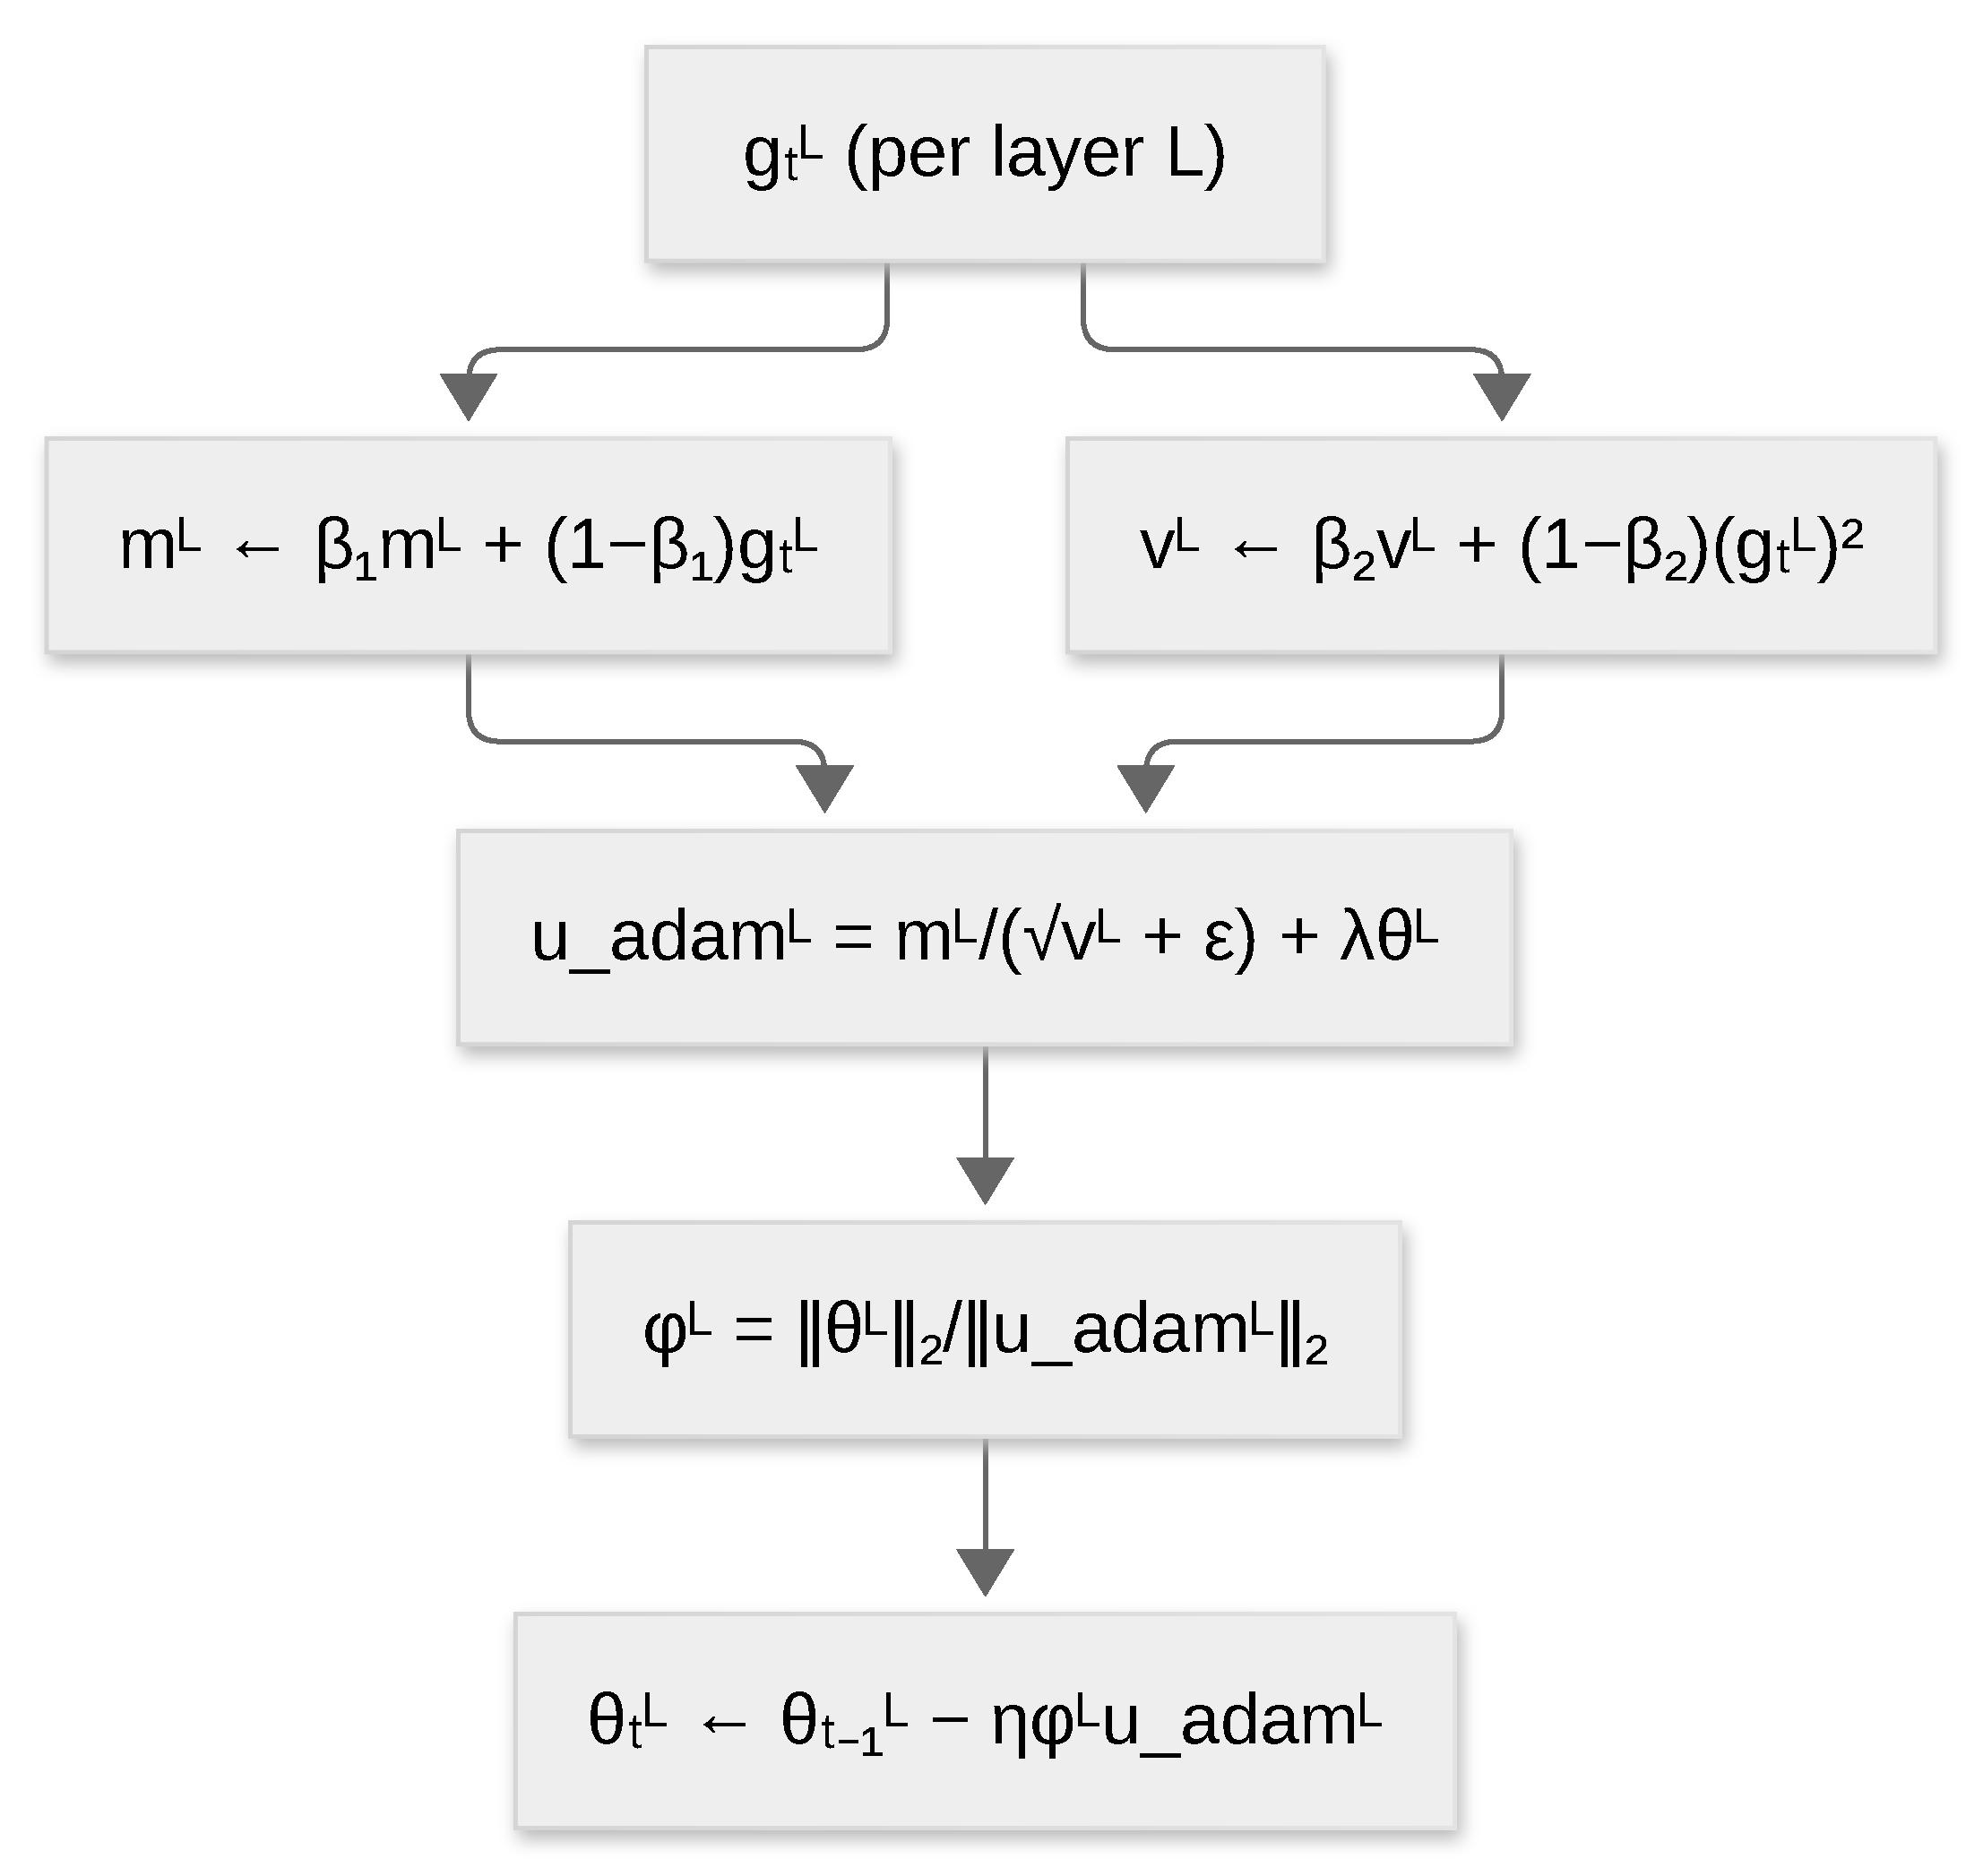
\includegraphics{../paper/figures/optimizers/lamb.pdf}}
\caption{Flujo por paso de LAMB: paso Adam por capas reescalado por la razón de confianza entre las normas de pesos y actualización.}
\label{fig:opt-lamb}
\end{figure}
LAMB extiende Adam con \textbf{escalado de tasa adaptativo por capas} (inspirado en LARS), permitiendo entrenamiento estable con tamaños de lote extremos (e.g., 64K en BERT):
\begin{align}
m_t^L &= \beta_1 m_{t-1}^L + (1-\beta_1)g_t^L \quad\text{(momento de primer orden por capas)} \\
v_t^L &= \beta_2 v_{t-1}^L + (1-\beta_2)(g_t^L)^2 \\
u_{\text{adam}}^L &= \frac{m_t^L}{\sqrt{v_t^L}+\epsilon} + \lambda\theta_{t-1}^L \quad\text{(paso adaptativo base con decaimiento)} \\
\phi^L &= \frac{\|\theta_{t-1}^L\|_2}{\|u_{\text{adam}}^L\|_2} \quad\text{(razón de confianza: normalización por capas)} \\
\theta_t^L &= \theta_{t-1}^L - \eta \cdot \phi^L \cdot u_{\text{adam}}^L
\end{align}
La \textbf{razón de confianza} $\phi^L = \|\theta^L\|_2 / \|u_{\text{adam}}^L\|_2$ normaliza el paso de actualización efectivo en relación con la magnitud de los pesos. En lotes muy grandes, el ruido estocástico del gradiente puede superar a la señal, desestabilizando las tasas de aprendizaje por capas. Al escalar las actualizaciones proporcionalmente a las normas de los pesos, LAMB asegura cambios relativos en lugar de absolutos, evitando que actualizaciones pequeñas y seguras en vectores grandes dominen.

\begin{algorithm}[H]
\caption{LAMB (Layer-wise Adaptive Moments optimizer for Batch training)}
\label{alg:lamb}
\begin{algorithmic}[1]
\Require Parámetros iniciales $\theta_0$, tasa de aprendizaje $\eta$, $\beta_1, \beta_2$, decaimiento de pesos $\lambda$
\Ensure Parámetros actualizados $\theta_T$
\State Inicializar: Para cada capa $L$: $m^L \gets 0$, $v^L \gets 0$
\For{$t = 1, 2, \ldots, T$}
    \For{cada capa $L$}
        \State $g_t^L \gets \nabla f(\theta_t^L)$
        \State $m^L \gets \beta_1 m^L + (1-\beta_1) g_t^L$
        \State $v^L \gets \beta_2 v^L + (1-\beta_2) (g_t^L)^2$
        \State Adam base: $u_{\text{adam}}^L \gets m^L / (\sqrt{v^L} + \epsilon)$
        \If{weight\_decay $> 0$}
            \State $u_{\text{adam}}^L \gets u_{\text{adam}}^L + \lambda \theta_{t-1}^L$
        \EndIf
        \State Razón de confianza: $\phi^L \gets \|\theta_{t-1}^L\|_2 / \|u_{\text{adam}}^L\|_2$ si ambos son no nulos, sino $1$
        \State $\theta_t^L \gets \theta_{t-1}^L - \eta \phi^L u_{\text{adam}}^L$
    \EndFor
\EndFor
\Return $\theta_T$
\end{algorithmic}
\end{algorithm}

\paragraph{Contras.}
\begin{itemize}[leftmargin=*]
\item La contabilidad de normas por capas y el cálculo de la razón de confianza añaden sobrecarga por paso.
\item La razón de confianza es inestable cuando las normas de capa o de actualización son cercanas a cero.
\end{itemize}

\paragraph{Ventajas.}
\begin{itemize}[leftmargin=*]
\item Permite entrenamiento estable con tamaños de lote extremos (e.g., 64K en BERT).
\item Preserva los beneficios de generalización de lotes pequeños mientras escala el lote.
\end{itemize}

\paragraph{Schedule-Free AdamW.}
\begin{figure}[H]
\centering
\fitfigure{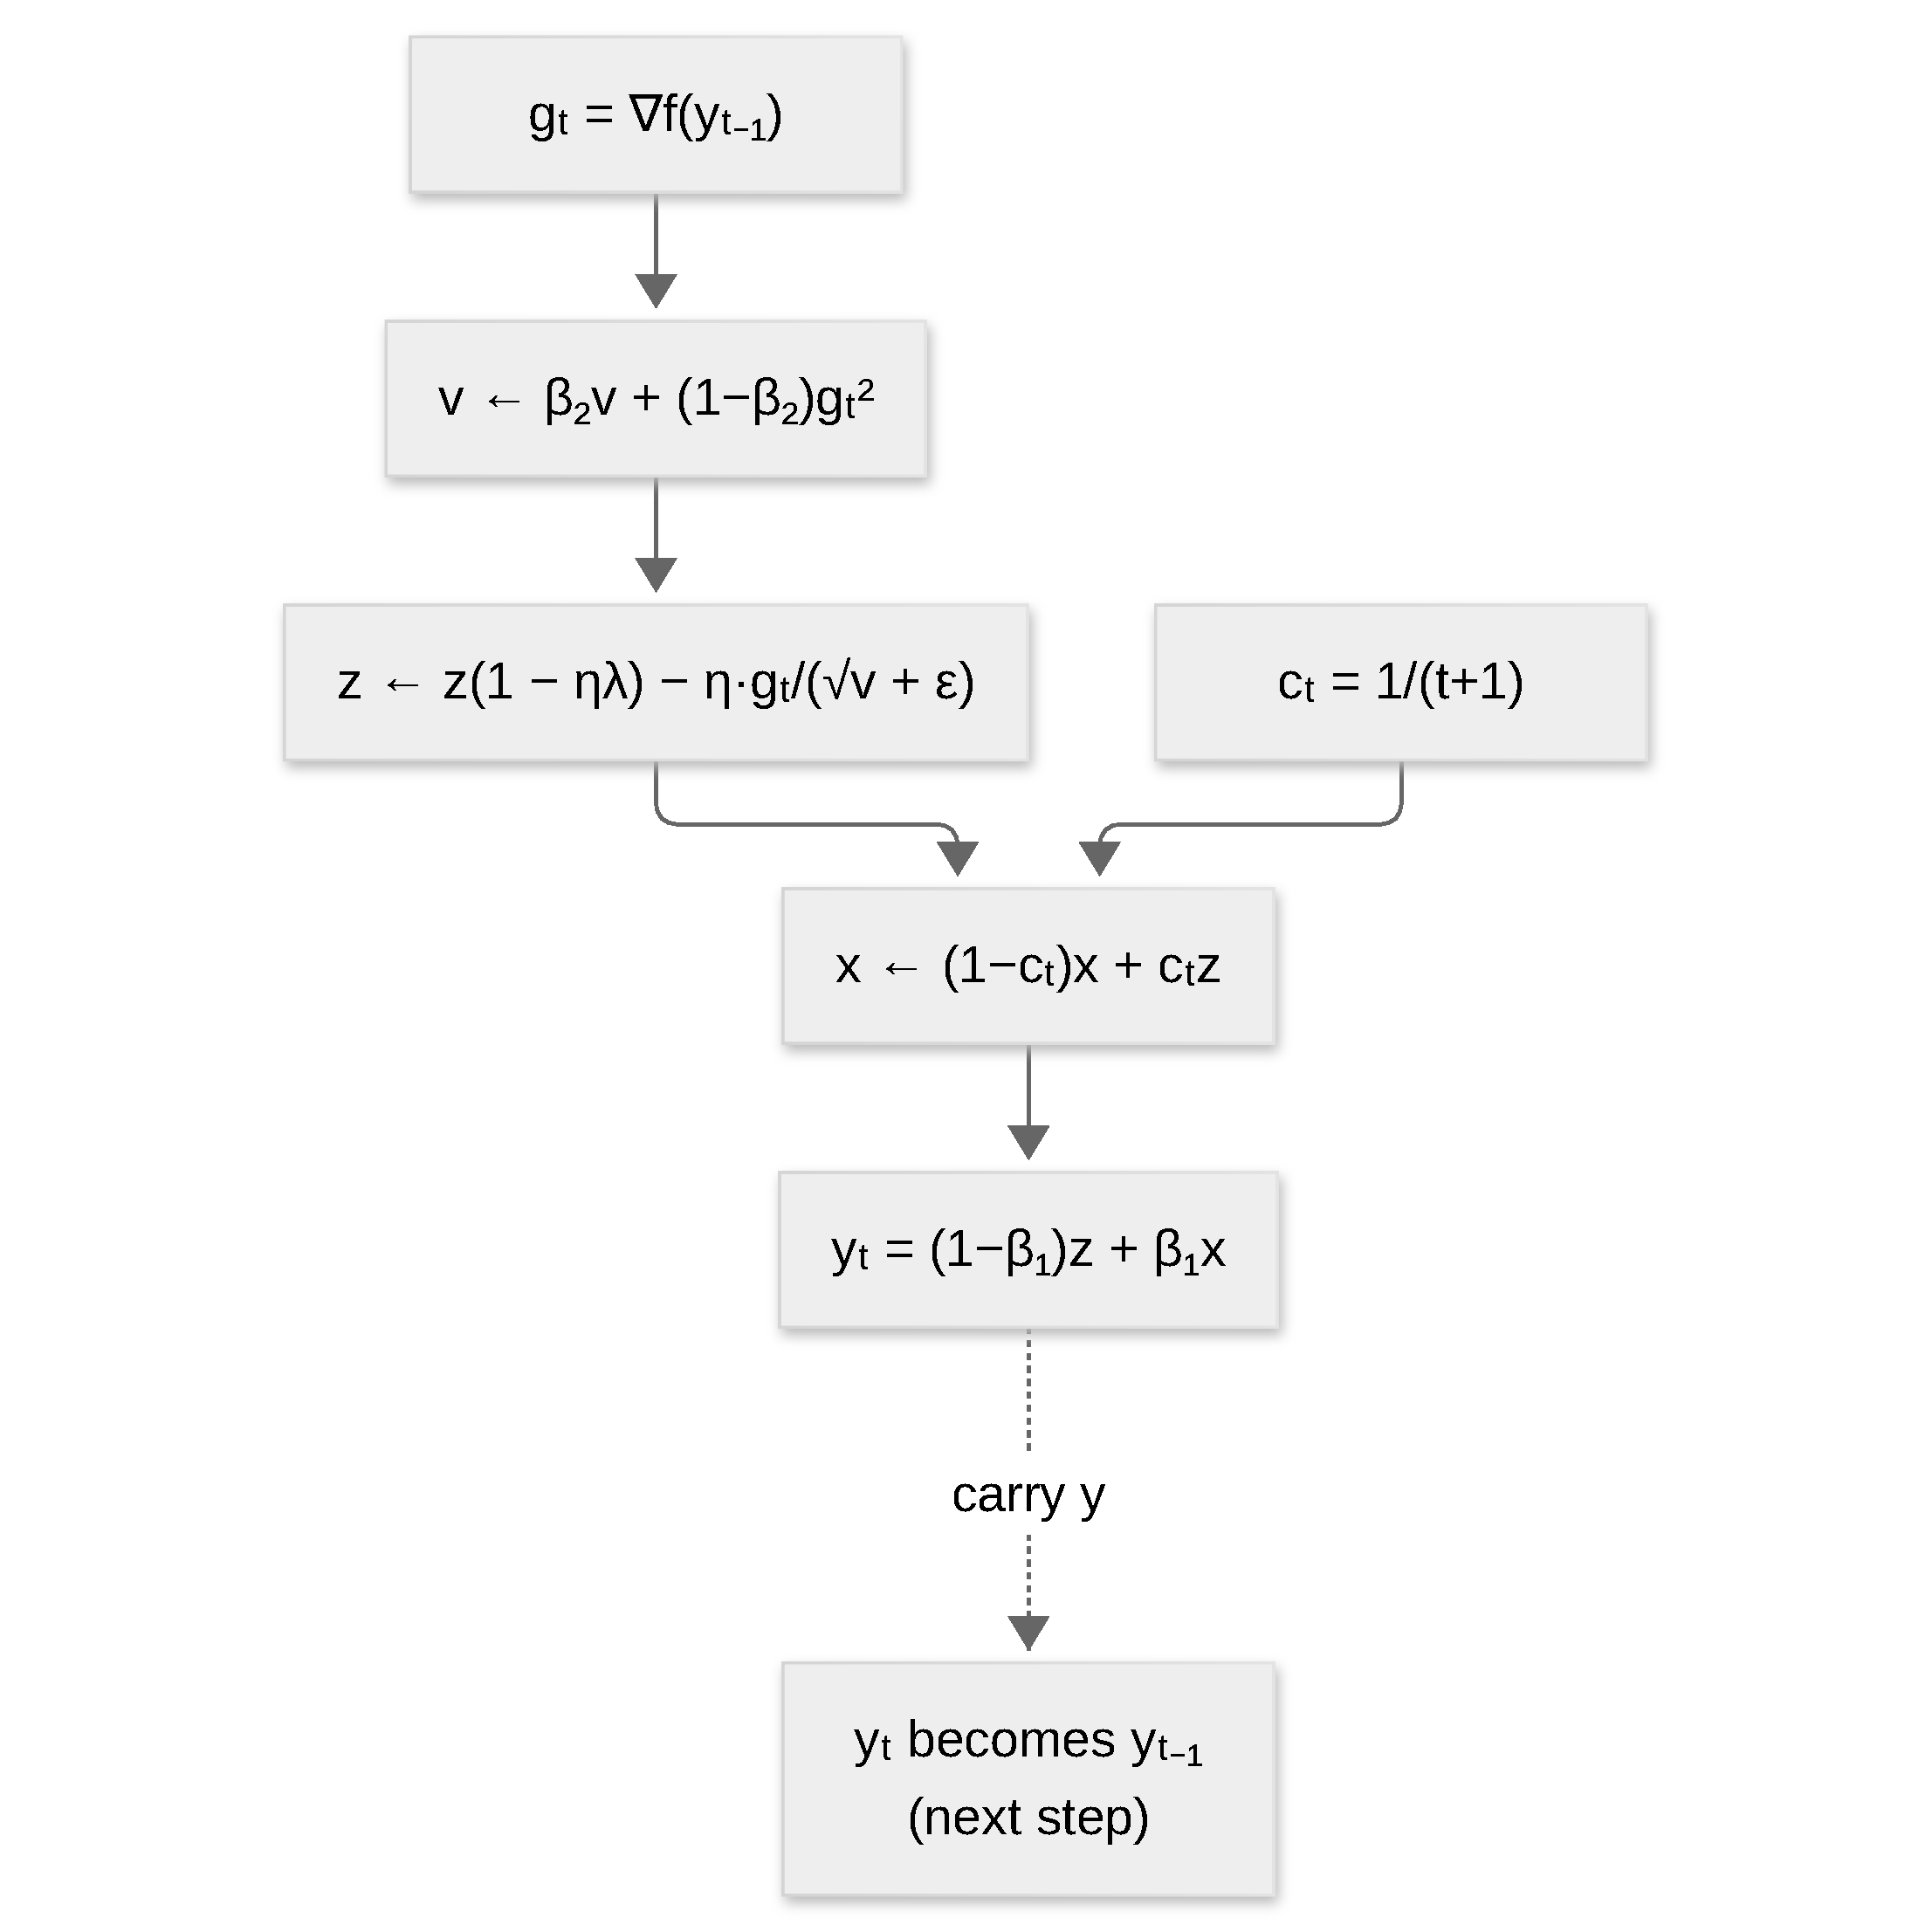
\includegraphics{../paper/figures/optimizers/schedulefree.pdf}}
\caption{Flujo por paso de Schedule-Free AdamW: flujo de exploración $z$, promedio de iteraciones $x$ y punto de interpolación $y$, con promediado implícito $1/(t+1)$.}
\label{fig:opt-schedulefree}
\end{figure}
Los métodos Schedule-Free eliminan el diseño explícito de programación de la receta de optimización. El algoritmo mantiene dos flujos de parámetros: $z_t$ (exploración) y $x_t$ (promedio suavizado):
\begin{align}
v_t &= \beta_2 v_{t-1} + (1-\beta_2)g_t^2 \quad\text{(varianza)} \\
z_t &= z_{t-1}(1-\eta\lambda) - \eta\frac{g_t}{\sqrt{v_t}+\epsilon} \quad\text{(paso adaptativo con decaimiento)} \\
c_t &= \frac{1}{t+1} \quad\text{(coeficiente de promediado, decrece con el tiempo)} \\
x_t &= (1-c_t)x_{t-1} + c_t z_t \quad\text{(promediado de iteraciones)} \\
y_t &= (1-\beta)z_t + \beta x_t \quad\text{(interpolación para el punto de evaluación)}
\end{align}
El coeficiente de promediado $c_t = 1/(t+1)$ implementa una programación de tasa de aprendizaje implícita sin especificar explícitamente el número total de pasos $T$. Este marco unifica la programación y el promediado de iteraciones: el algoritmo explora mediante $z_t$ mientras acumula dirección estable mediante $x_t$. El punto de evaluación $y_t$ (usado para el cómputo del gradiente) interpola entre exploración y estabilidad.

\begin{algorithm}[H]
\caption{Schedule-Free AdamW}
\label{alg:schedulefree}
\begin{algorithmic}[1]
\Require Parámetros iniciales $\theta_0$, tasa de aprendizaje $\eta$ (fija), $\beta_1, \beta_2$, decaimiento de pesos $\lambda$
\Ensure Parámetros actualizados $\theta_T$ o promediado $x_T$
\State Inicializar: $z \gets \theta_0$ (exploración), $x \gets \theta_0$ (promedio), $v \gets 0$, $t \gets 0$
\For{$t = 1, 2, \ldots, T$}
    \State $g_t \gets \nabla f(y_{t-1})$ (gradiente en el punto de interpolación)
    \State $v \gets \beta_2 v + (1-\beta_2) g_t^2$ \Comment{Varianza}
    \State Decaimiento de pesos sobre $z$: $z \gets z(1 - \eta\lambda)$
    \State $z \gets z - \eta g_t / (\sqrt{v} + \epsilon)$ \Comment{Paso adaptativo sobre el gradiente crudo}
    \State $c_t \gets 1 / (t+1)$ \Comment{Coeficiente de promediado}
    \State $x \gets (1-c_t) x + c_t z$ \Comment{Promediado de iteraciones}
    \State $y_t \gets (1-\beta_1) z + \beta_1 x$ \Comment{Interpolación para la siguiente evaluación}
\EndFor
\Return $x_T$ o $y_T$
\end{algorithmic}
\end{algorithm}

\paragraph{Contras.}
\begin{itemize}[leftmargin=*]
\item Mantiene dos flujos de parámetros ($z$ y $x$) y requiere manejar explícitamente el punto de evaluación.
\item Su comportamiento difiere de las líneas base con programación, lo que complica las comparaciones.
\end{itemize}

\paragraph{Ventajas.}
\begin{itemize}[leftmargin=*]
\item Elimina la programación explícita de la tasa de aprendizaje y su hiperparámetro de pasos totales.
\item Convergencia de última generación en optimización convexa, aprendizaje profundo a gran escala y aprendizaje por refuerzo.
\end{itemize}

\paragraph{Adafactor.}
\begin{figure}[H]
\centering
\fitfigure{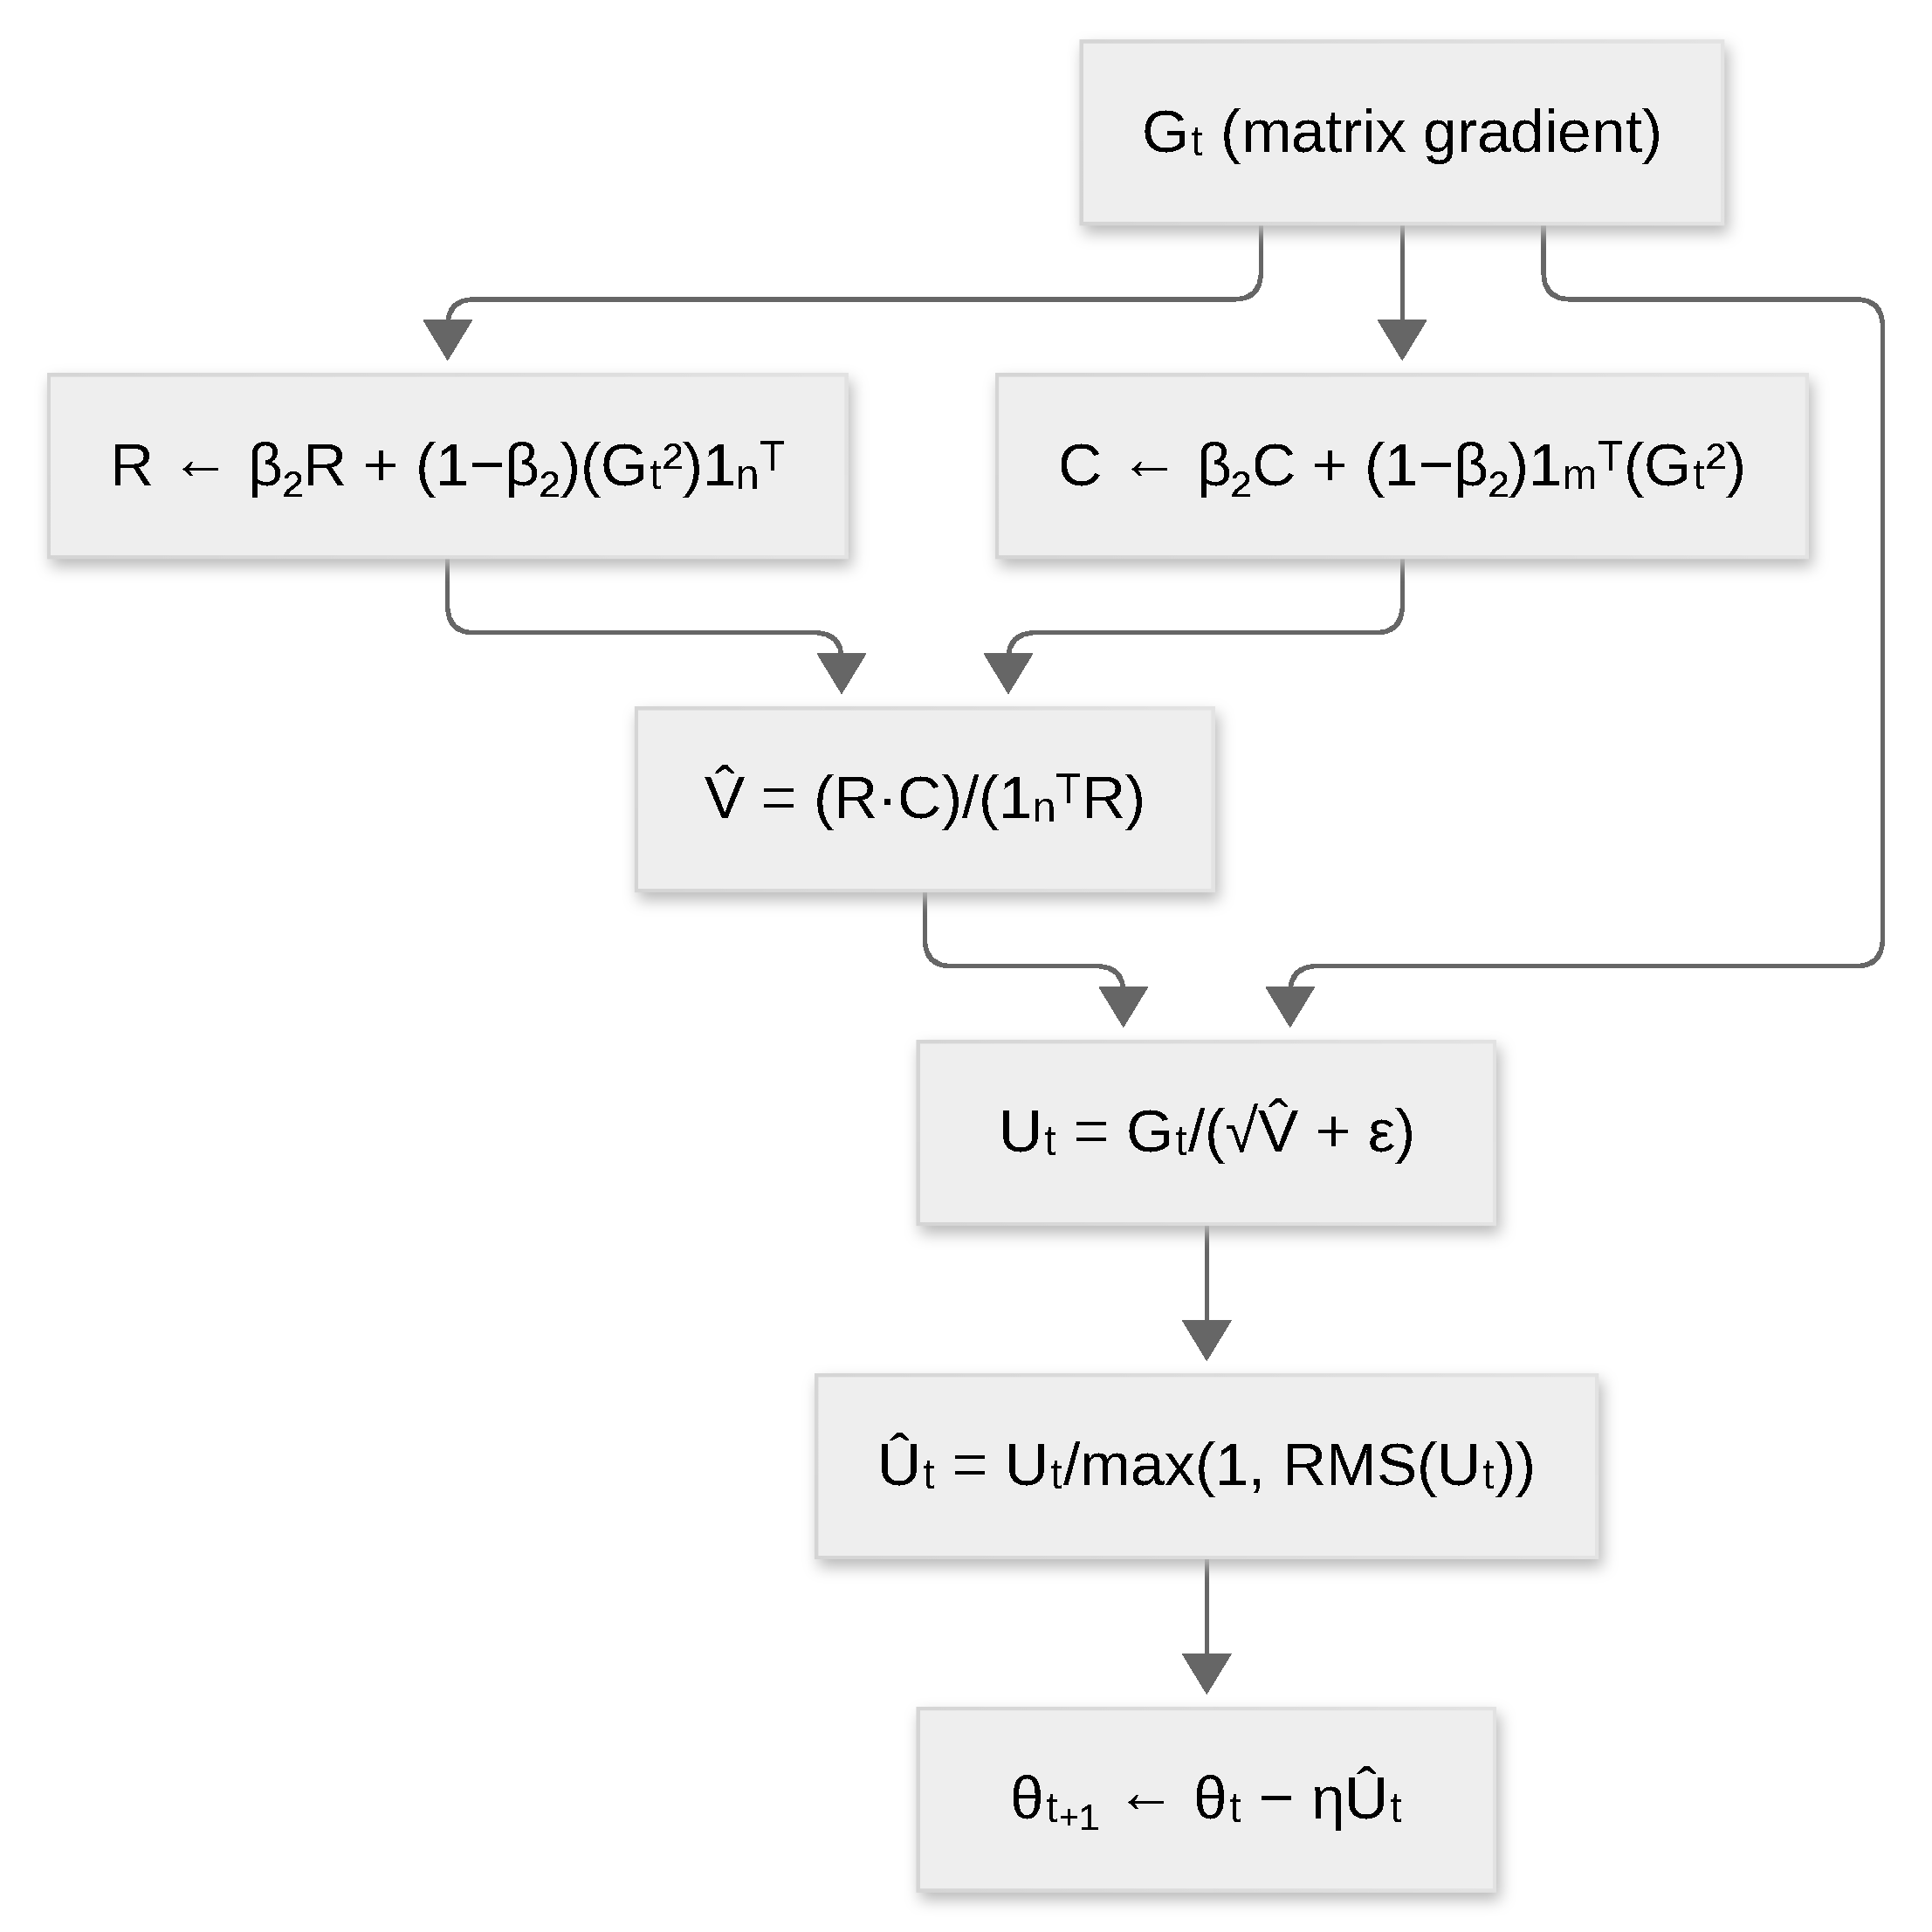
\includegraphics{../paper/figures/optimizers/adafactor.pdf}}
\caption{Flujo por paso de Adafactor: acumuladores factorizados de segundo momento por filas y columnas, reconstrucción mediante producto exterior y recorte RMS.}
\label{fig:opt-adafactor}
\end{figure}
Adafactor reduce la memoria del optimizador \textbf{factorizando} estadísticas de segundo momento para parámetros con forma de matriz, almacenando solo acumuladores de filas y columnas en lugar de estados de varianza densos. Para una matriz de gradiente $G_t \in \mathbb{R}^{m \times n}$:
\begin{align}
R_t &= \beta_2 R_{t-1} + (1-\beta_2)(G_t^2) \mathbf{1}_n^T \quad\text{(varianza por filas)} \\
C_t &= \beta_2 C_{t-1} + (1-\beta_2) \mathbf{1}_m^\top (G_t^2) \quad\text{(varianza por columnas)} \\
\hat{V}_t &= \frac{R_t C_t}{\mathbf{1}_n^\top R_t} \quad\text{(varianza reconstruida mediante producto exterior)} \\
U_t &= \frac{G_t}{\sqrt{\hat{V}_t}+\epsilon} \quad\text{(paso adaptativo normalizado)} \\
\hat{U}_t &= \frac{U_t}{\max(1, \text{RMS}(U_t))} \quad\text{(recorte de estabilidad)}
\end{align}

\begin{algorithm}[H]
\caption{Adafactor (Estadísticas de Segundo Momento Factorizadas)}
\label{alg:adafactor}
\begin{algorithmic}[1]
\Require Matriz de gradiente $G_t \in \mathbb{R}^{m \times n}$, tasa de aprendizaje $\eta$, $\beta_2 \approx 0.999$
\Ensure Parámetros actualizados $\theta_T$
\State Inicializar: Acumuladores de fila $R \gets \epsilon \mathbf{1}^T_m$, Columna $C \gets \epsilon \mathbf{1}_n$
\For{$t = 1, 2, \ldots, T$}
    \State $G_t \gets \nabla f(\theta_t)$ (gradiente matricial)
    \State $R \gets \beta_2 R + (1-\beta_2) (G_t^2) \mathbf{1}_n^T$ \Comment{Productos internos por filas}
    \State $C \gets \beta_2 C + (1-\beta_2) \mathbf{1}_m^\top (G_t^2)$ \Comment{Productos internos por columnas}
    \State Varianza reconstruida: $\hat{V} \gets (R \cdot C) / (\mathbf{1}_n^\top R)$ \Comment{Mediante producto exterior}
    \State Paso adaptativo normalizado: $U_t \gets G_t / (\sqrt{\hat{V}} + \epsilon)$
    \State Recorte RMS por fila: $\hat{U}_t \gets U_t / \max(1, \text{RMS}(U_t))$
    \State $\theta_{t+1} \gets \theta_t - \eta \hat{U}_t$
\EndFor
\Return $\theta_T$
\end{algorithmic}
\end{algorithm}

\paragraph{Contras.}
\begin{itemize}[leftmargin=*]
\item La varianza factorizada es una aproximación y puede ser inestable en algunas tareas.
\item Menor expresividad de optimización en comparación con Adam completo.
\end{itemize}

\paragraph{Ventajas.}
\begin{itemize}[leftmargin=*]
\item La memoria baja de $O(n_{\text{params}})$ a $O(\sqrt{n_{\text{params}}})$ para parámetros matriciales.
\item Más atractivo cuando la VRAM está dominada por el estado del optimizador en lugar de las activaciones.
\end{itemize}

\paragraph{GaLore (Gradient Low-Rank Projection).}
\begin{figure}[H]
\centering
\fitfigure{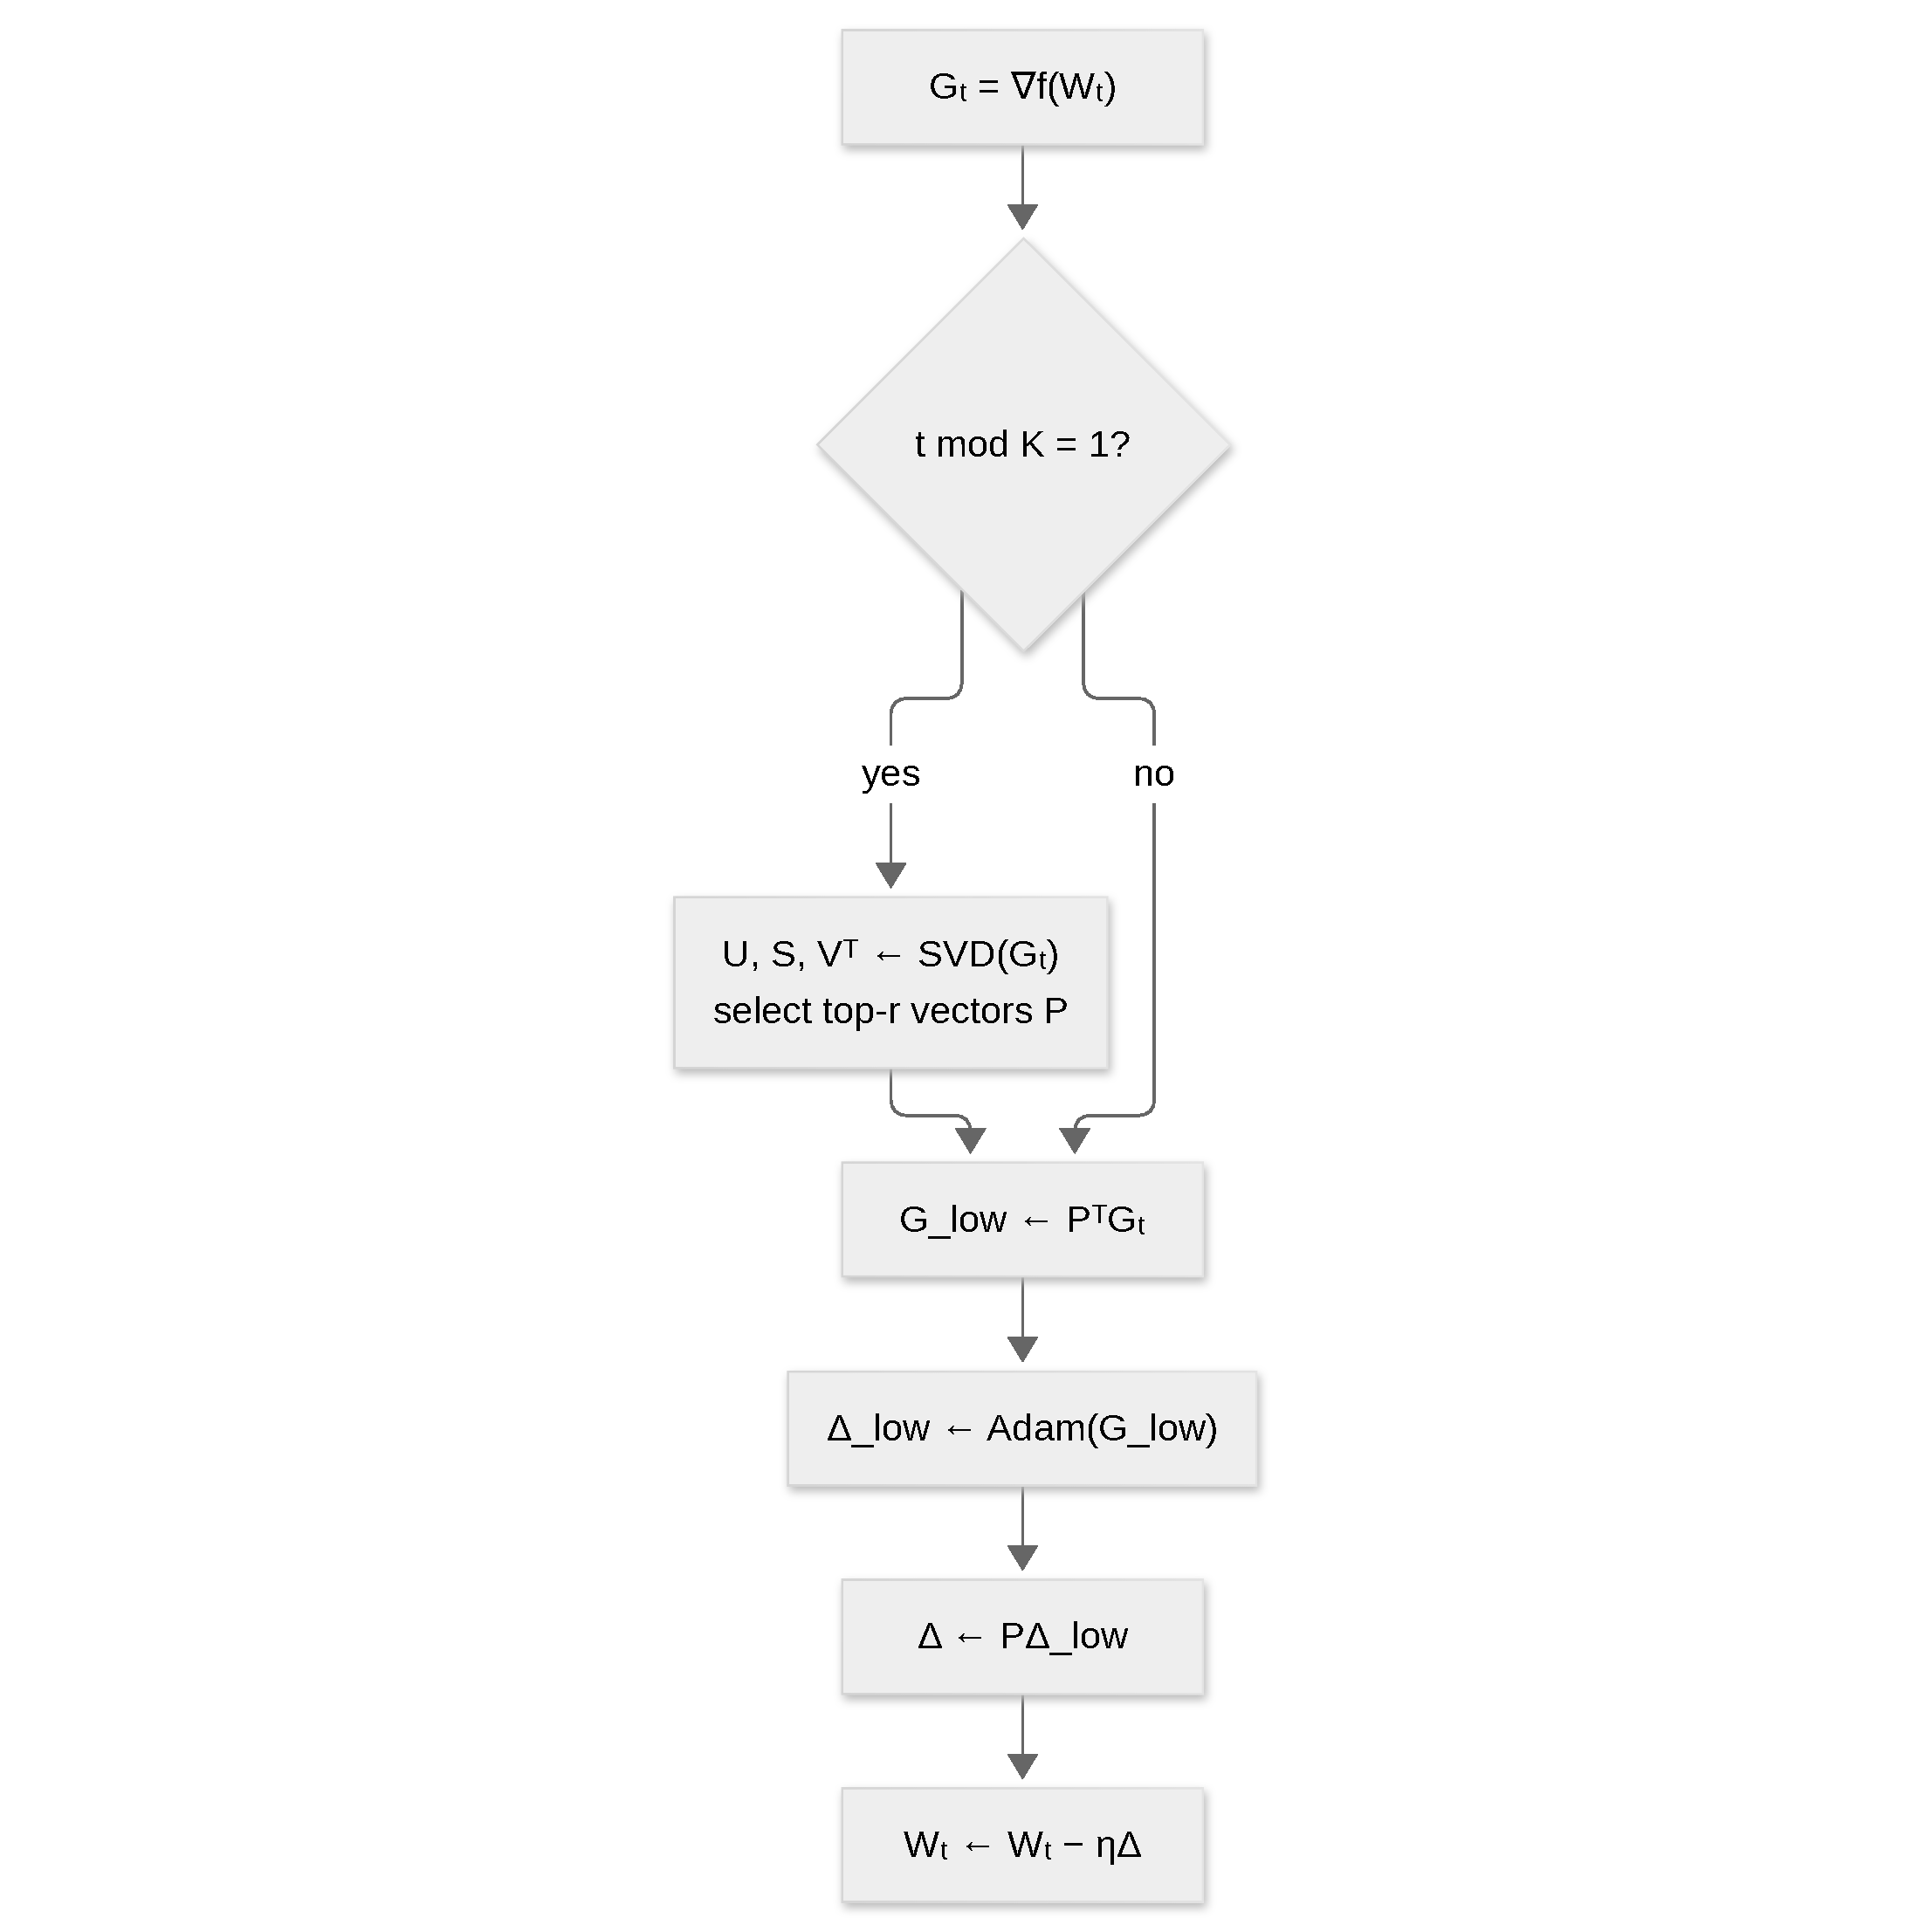
\includegraphics{../paper/figures/optimizers/galore.pdf}}
\caption{Flujo por paso de GaLore: proyección SVD periódica del gradiente a un subespacio de bajo rango, Adam en ese subespacio y reconstrucción.}
\label{fig:opt-galore}
\end{figure}
GaLore proyecta gradientes 2D en un subespacio de bajo rango antes de la optimización, reduciendo la memoria del estado del optimizador mientras mantiene el escalado adaptativo del paso. Para una matriz de parámetros 2D $W \in \mathbb{R}^{m \times n}$:
\begin{align}
U, S, V &= \text{SVD}(G_t) \quad\text{(calcular descomposición singular)} \\
P &\in \mathbb{R}^{n \times r} \quad\text{o} \quad P^\top \in \mathbb{R}^{r \times m} \quad\text{(seleccionar los $r$ vectores singulares superiores)} \\
G_{\text{low}} &= P^\top G_t \quad\text{(proyectar al espacio de bajo rango)} \\
\Delta_{\text{low}} &= \text{Adam}(G_{\text{low}}) \quad\text{(optimizar en el espacio comprimido)} \\
\Delta &= P \Delta_{\text{low}} \quad\text{(reconstruir en el espacio original)}
\end{align}
Al proyectar en un subespacio de rango $r$ (típicamente $r \ll \min(m,n)$), el estado del optimizador se reduce de $O(mn)$ a $O(r(m+n))$ para parámetros 2D. Este enfoque complementario de ahorro de memoria es especialmente relevante cuando el modelo es demasiado grande para el estado completo del optimizador.

\begin{algorithm}[H]
\caption{GaLore (Gradient Low-Rank Projection)}
\label{alg:galore}
\begin{algorithmic}[1]
\Require Matriz de parámetros 2D $W \in \mathbb{R}^{m \times n}$, tasa de aprendizaje $\eta$, rango $r \ll \min(m,n)$
\Ensure Parámetros actualizados $\theta_T$
\State Inicializar: Estado de Adam en el espacio de bajo rango (si es variante de rango 2)
\For{$t = 1, 2, \ldots, T$}
    \State $G_t \gets \nabla f(W_t)$
    \If{$t \mod K = 1$}  \Comment{SVD periódico}
        \State $U_t, S_t, V_t^\top \gets \text{SVD}(G_t)$ (completa o delgada)
        \State Seleccionar proyección: $P \gets U_t[:, :r]$ o $P \gets V_t[:, :r]$
    \EndIf
    \State Proyectar gradiente: $G_{\text{low}} \gets P^\top G_t$ (o $G_t P^\top$ para proyección derecha)
    \State Ejecutar Adam en bajo rango: $\Delta_{\text{low}} \gets \text{Adam}(G_{\text{low}})$
    \State Reconstruir en espacio original: $\Delta \gets P \Delta_{\text{low}}$ (o $\Delta_{\text{low}} P^\top$)
    \State $W_t \gets W_t - \eta \Delta$
\EndFor
\Return $\theta_T$
\end{algorithmic}
\end{algorithm}

\paragraph{Contras.}
\begin{itemize}[leftmargin=*]
\item El SVD periódico añade cómputo e introduce un intervalo de actualización de la proyección que ajustar.
\item La proyección de bajo rango puede descartar información del gradiente.
\end{itemize}

\paragraph{Ventajas.}
\begin{itemize}[leftmargin=*]
\item El estado del optimizador se reduce de $O(mn)$ a $O(r(m+n))$ para parámetros 2D.
\item Funciona sinérgicamente con otras técnicas y ha mostrado resultados sólidos en modelos de miles de millones de parámetros.
\end{itemize}

\paragraph{APOLLO, APOLLO-Mini, y Q-APOLLO.}
\begin{figure}[H]
\centering
\fitfigure{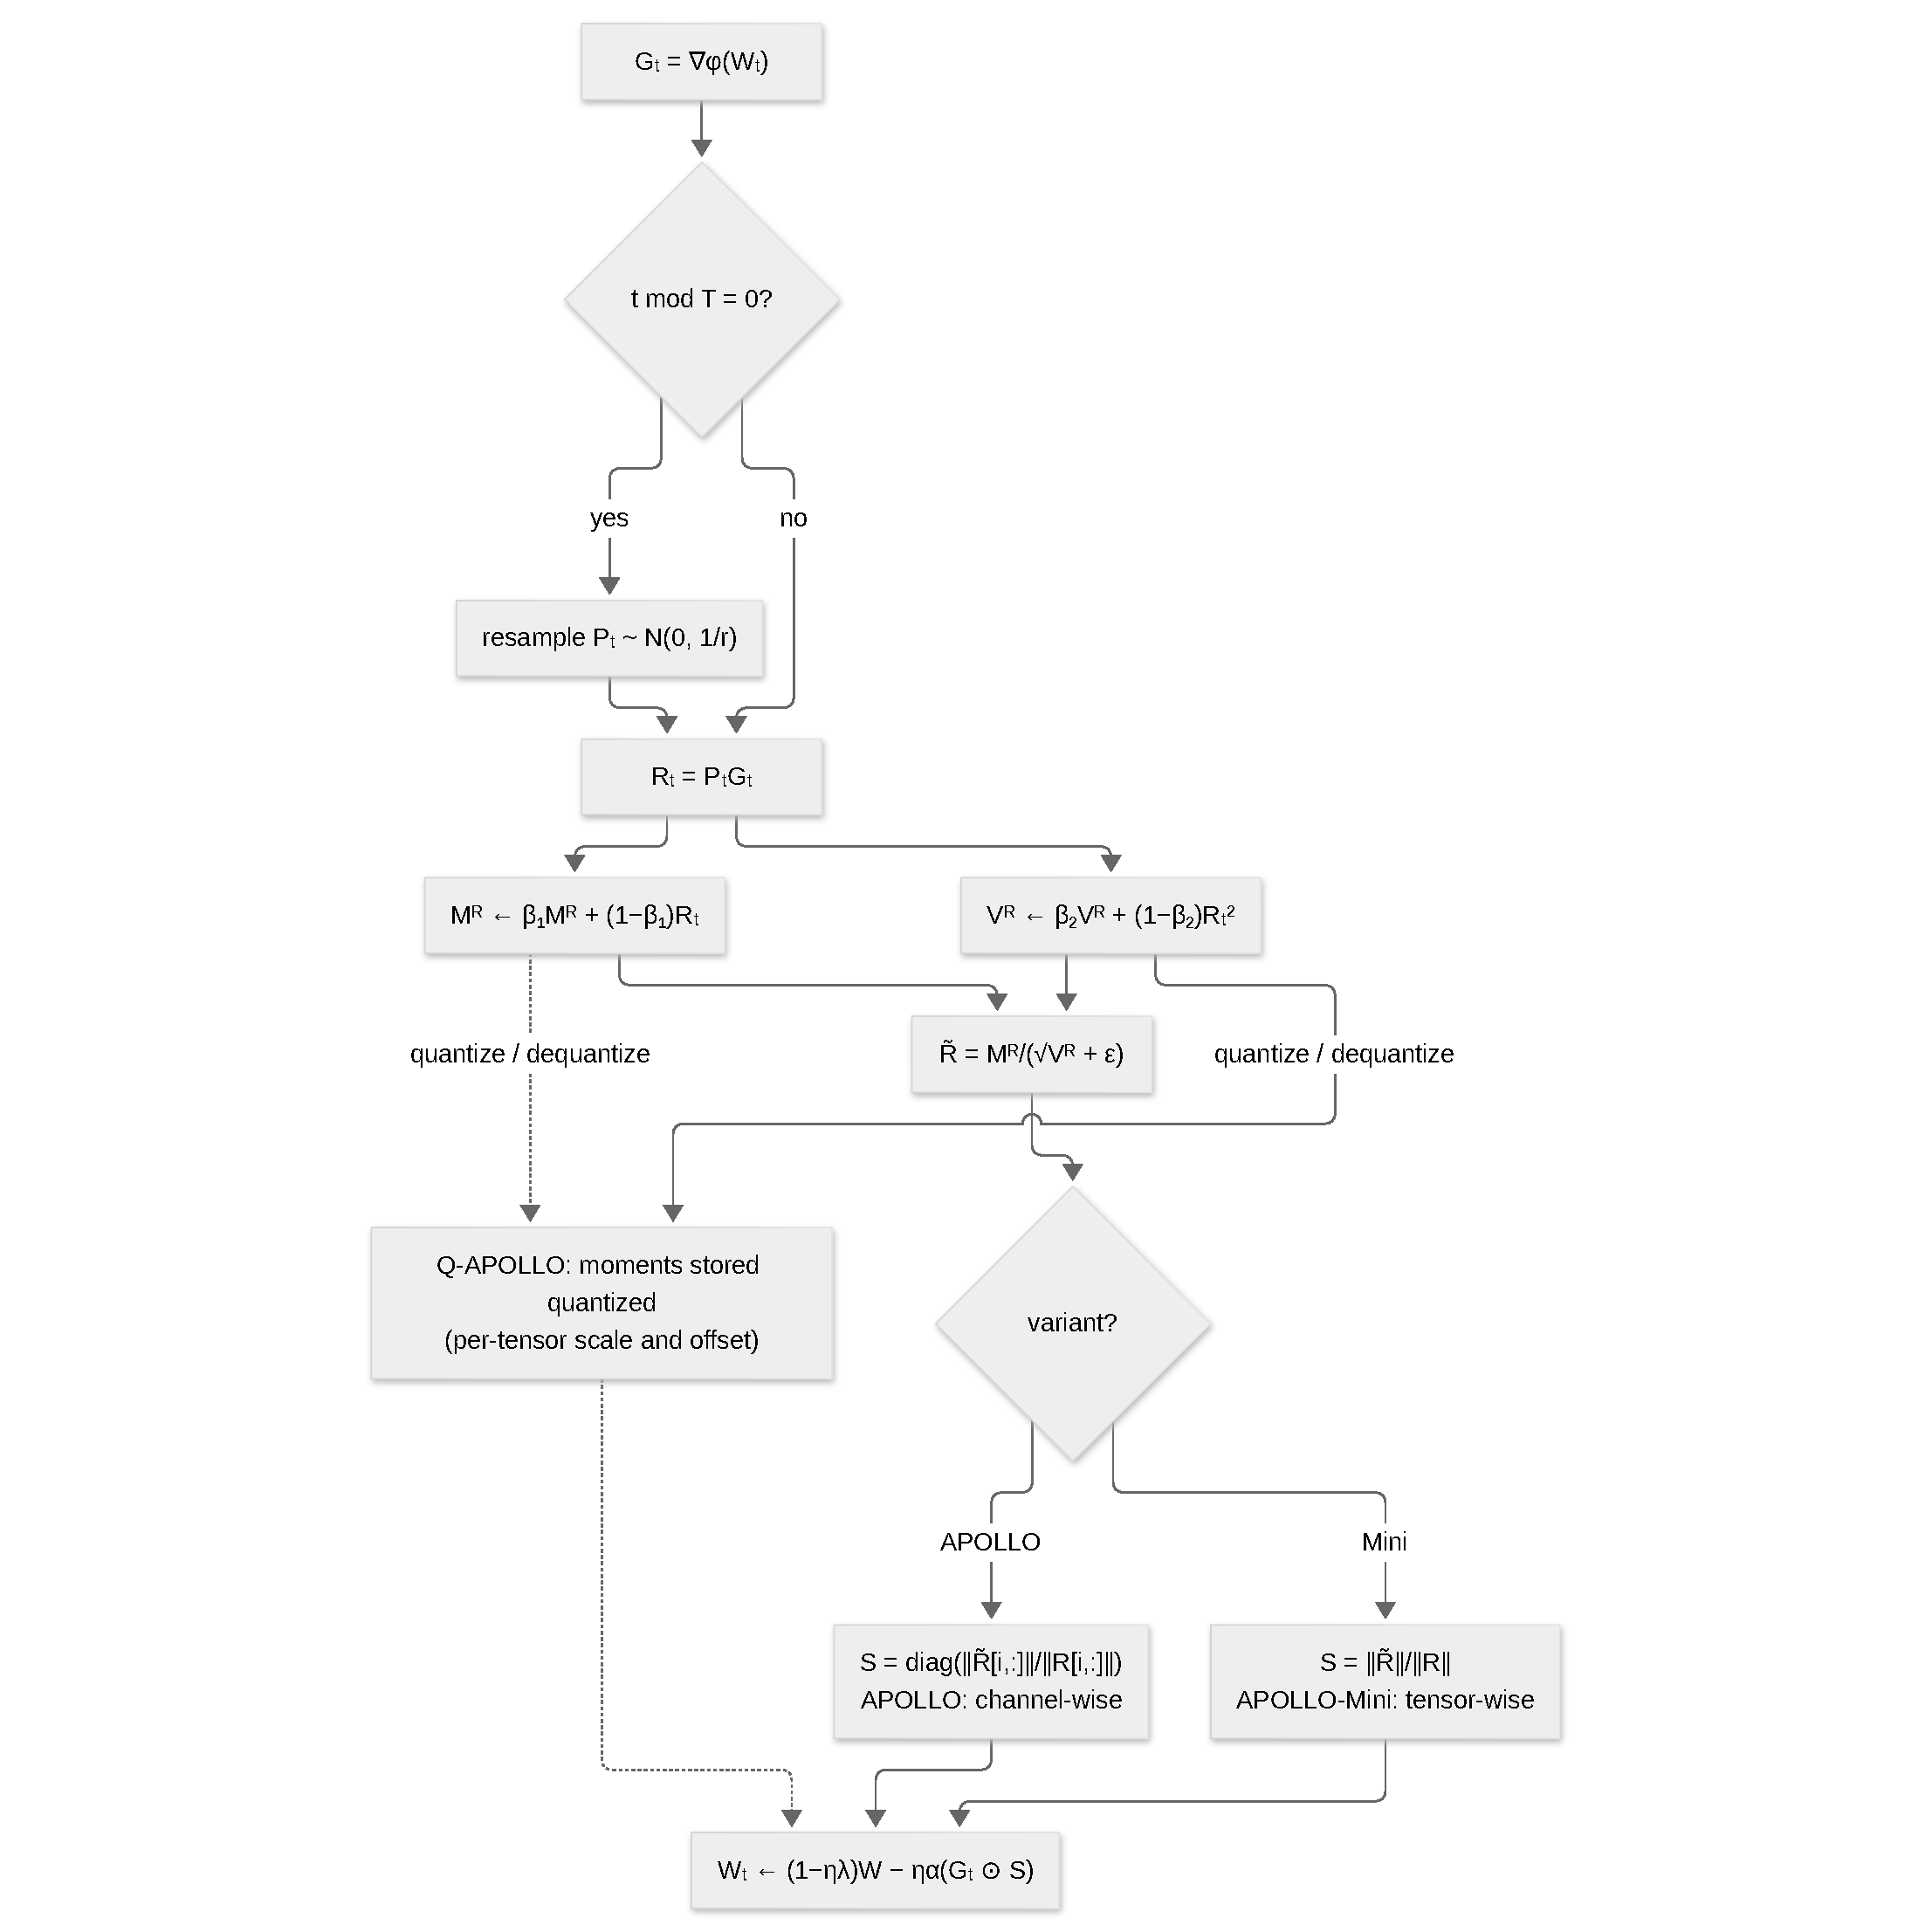
\includegraphics{../paper/figures/optimizers/apollo.pdf}}
\caption{Flujo por paso de la familia APOLLO: momentos proyectados gaussianos, escalado estructurado del gradiente (por canales en APOLLO, escalar en APOLLO-Mini) y estado cuantizado en Q-APOLLO.}
\label{fig:opt-apollo}
\end{figure}
La familia APOLLO \citep{zhu2025apollosgdlikememoryadamwlevel} parte de la observación de que el denominador elemento a elemento de AdamW puede \textbf{transformarse en una actualización estructurada de la tasa de aprendizaje}. En lugar de almacenar momentos densos para cada entrada de parámetro, APOLLO proyecta un gradiente matricial $G_t \in \mathbb{R}^{m \times n}$ en un subespacio aleatorio compacto y rastrea momentos estilo Adam allí:
\begin{align}
R_t &= P_t G_t \quad\text{o}\quad R_t = G_t P_t^\top \\
M_t^R &= \beta_1 M_{t-1}^R + (1-\beta_1)R_t \\
V_t^R &= \beta_2 V_{t-1}^R + (1-\beta_2)R_t^2 \\
\widetilde{R}_t &= \frac{M_t^R}{\sqrt{V_t^R}+\epsilon}
\end{align}
El estado proyectado \emph{no} se expande de vuelta a una actualización densa de bajo rango como en los métodos basados en SVD. En su lugar, APOLLO estima un tensor de escalado estructurado $S_t$ en el espacio original. En la variante estándar de APOLLO, ese escalado es \textbf{por canales}: cada fila o canal recibe su propia razón de norma. En APOLLO-Mini, el escalado se reduce a un único escalar \textbf{por tensor}, correspondiente al caso extremo de rango 1 descrito en el artículo. La actualización de parámetros resultante es, por tanto, similar a Adam en adaptación pero mucho más cercana a SGD en costo de estado:
\[
W_t \gets (1-\eta\lambda)W_{t-1} - \eta\,\alpha\,(G_t \odot S_t)
\]
donde $\alpha$ es el factor de escala adicional usado para estabilizar variantes altamente comprimidas.

\begin{algorithm}[H]
\caption{APOLLO / APOLLO-Mini Escalado de Gradiente Estructurado}
\label{alg:apollo-family}
\begin{algorithmic}[1]
\Require Matriz de pesos $W \in \mathbb{R}^{m \times n}$ con $m \le n$, tasa de aprendizaje $\eta$, factor de escala $\alpha$, tasas de decaimiento $(\beta_1, \beta_2)$, decaimiento de pesos $\lambda$, rango $r$, intervalo de actualización de proyección $T$
\Ensure Parámetros actualizados $W_T$
\State Inicializar momentos proyectados: $M^R \gets 0$, $V^R \gets 0$, paso $t \gets 0$
\Repeat
    \State Calcular gradiente: $G_t \gets \nabla_W \phi(W_t)$
    \If{$t \bmod T = 0$}
        \State Muestrear proyector gaussiano $P_t \sim \mathcal{N}(0, 1/r)$ con una semilla nueva
    \EndIf
    \State Proyectar gradiente: $R_t \gets P_t G_t$ \Comment{o $G_t P_t^\top$ según la disposición}
    \State Actualizar momentos proyectados AdamW: $M_t^R, V_t^R \gets \text{AdamWState}(R_t; \beta_1, \beta_2)$
    \State Normalizar estado proyectado: $\widetilde{R}_t \gets M_t^R / (\sqrt{V_t^R}+\epsilon)$
    \If{APOLLO}
        \State $S_t \gets \operatorname{diag}(s_1^R, \ldots, s_m^R)$, donde $s_i^R = \|\widetilde{R}_t[i,:]\|_2 / \|R_t[i,:]\|_2$
    \Else
        \State $S_t \gets s_t^R$, donde $s_t^R = \|\widetilde{R}_t\|_2 / \|R_t\|_2$
    \EndIf
    \State Actualizar pesos: $W_t \gets (1-\eta\lambda)W_{t-1} - \eta\,\alpha\,(G_t \odot S_t)$
    \State $t \gets t+1$
\Until{convergencia}
\end{algorithmic}
\end{algorithm}

\paragraph{Contras.}
\begin{itemize}[leftmargin=*]
\item El escalado estructurado es una aproximación más gruesa del denominador elemento a elemento de AdamW.
\item Las proyecciones deben refrescarse periódicamente y rangos muy pequeños hacen que el escalado sea ruidoso.
\end{itemize}

\paragraph{Ventajas.}
\begin{itemize}[leftmargin=*]
\item Reemplaza el SVD repetido con proyección aleatoria gaussiana refrescada periódicamente, de modo que el costo de sistemas es multiplicación de matrices ordinaria en lugar de descomposición espectral.
\item Inusualmente tolerante a la compresión extrema: incluso APOLLO-Mini, que solo mantiene estado auxiliar de rango 1, sigue siendo competitivo o mejor que AdamW mientras se acerca al costo de memoria de SGD.
\end{itemize}

\paragraph{APOLLO-Mini.}
APOLLO-Mini es el miembro de la familia optimizado para \textbf{eficiencia de memoria extrema}. El artículo lo motiva argumentando que, en un espacio compacto de rango 1, el escalado por canales se vuelve demasiado ruidoso, por lo que la actualización se simplifica aún más a un único escalar por tensor. La pérdida de granularidad se compensa parcialmente con el factor de escala explícito $\alpha$ (el artículo discute valores como $128$ en este régimen), proporcionando un punto útil en la frontera de Pareto de optimización: estado muy pequeño, sin sobrecarga de SVD, y aún un comportamiento sólido en preentrenamiento.

\paragraph{Contras.}
\begin{itemize}[leftmargin=*]
\item Un único escalar por tensor pierde granularidad por canales, y el estado de rango 1 puede ser ruidoso.
\item Depende del factor de escala adicional $\alpha$ (e.g., $128$) para mantenerse estable.
\end{itemize}

\paragraph{Ventajas.}
\begin{itemize}[leftmargin=*]
\item El estado más pequeño de la familia APOLLO, sin sobrecarga de SVD.
\item Comportamiento sólido en preentrenamiento con un costo de memoria cercano a SGD.
\end{itemize}

\paragraph{Q-APOLLO.}
El artículo de APOLLO también enfatiza que la familia se combina naturalmente con \textbf{cuantización} para entrenamiento con memoria ultra-baja. Este repositorio convierte esa observación de sistemas en una variante concreta del optimizador, \texttt{q\_apollo}. En la implementación, los momentos de primer y segundo orden de bajo rango de APOLLO se almacenan en forma cuantizada junto con escalas y desplazamientos por tensor, y se descuantizan solo cuando es necesario para el siguiente paso. Q-APOLLO preserva, por tanto, la lógica de gradiente proyectado de APOLLO mientras reduce la precisión del estado restante del optimizador.

\paragraph{Contras.}
\begin{itemize}[leftmargin=*]
\item Los momentos cuantizados introducen error de aproximación y sobrecarga de descuantización.
\item Requiere gestionar escalas y desplazamientos por tensor.
\end{itemize}

\paragraph{Ventajas.}
\begin{itemize}[leftmargin=*]
\item Reduce el estado restante del optimizador a precisión ultra baja.
\item Miembro más agresivo en ahorro de memoria de la pila local, preservando la lógica de gradiente proyectado de APOLLO.
\end{itemize}

\paragraph{Anon (Adaptivity Non-restricted Optimizer with Novel convergence technique).}
\begin{figure}[H]
\centering
\fitfigure{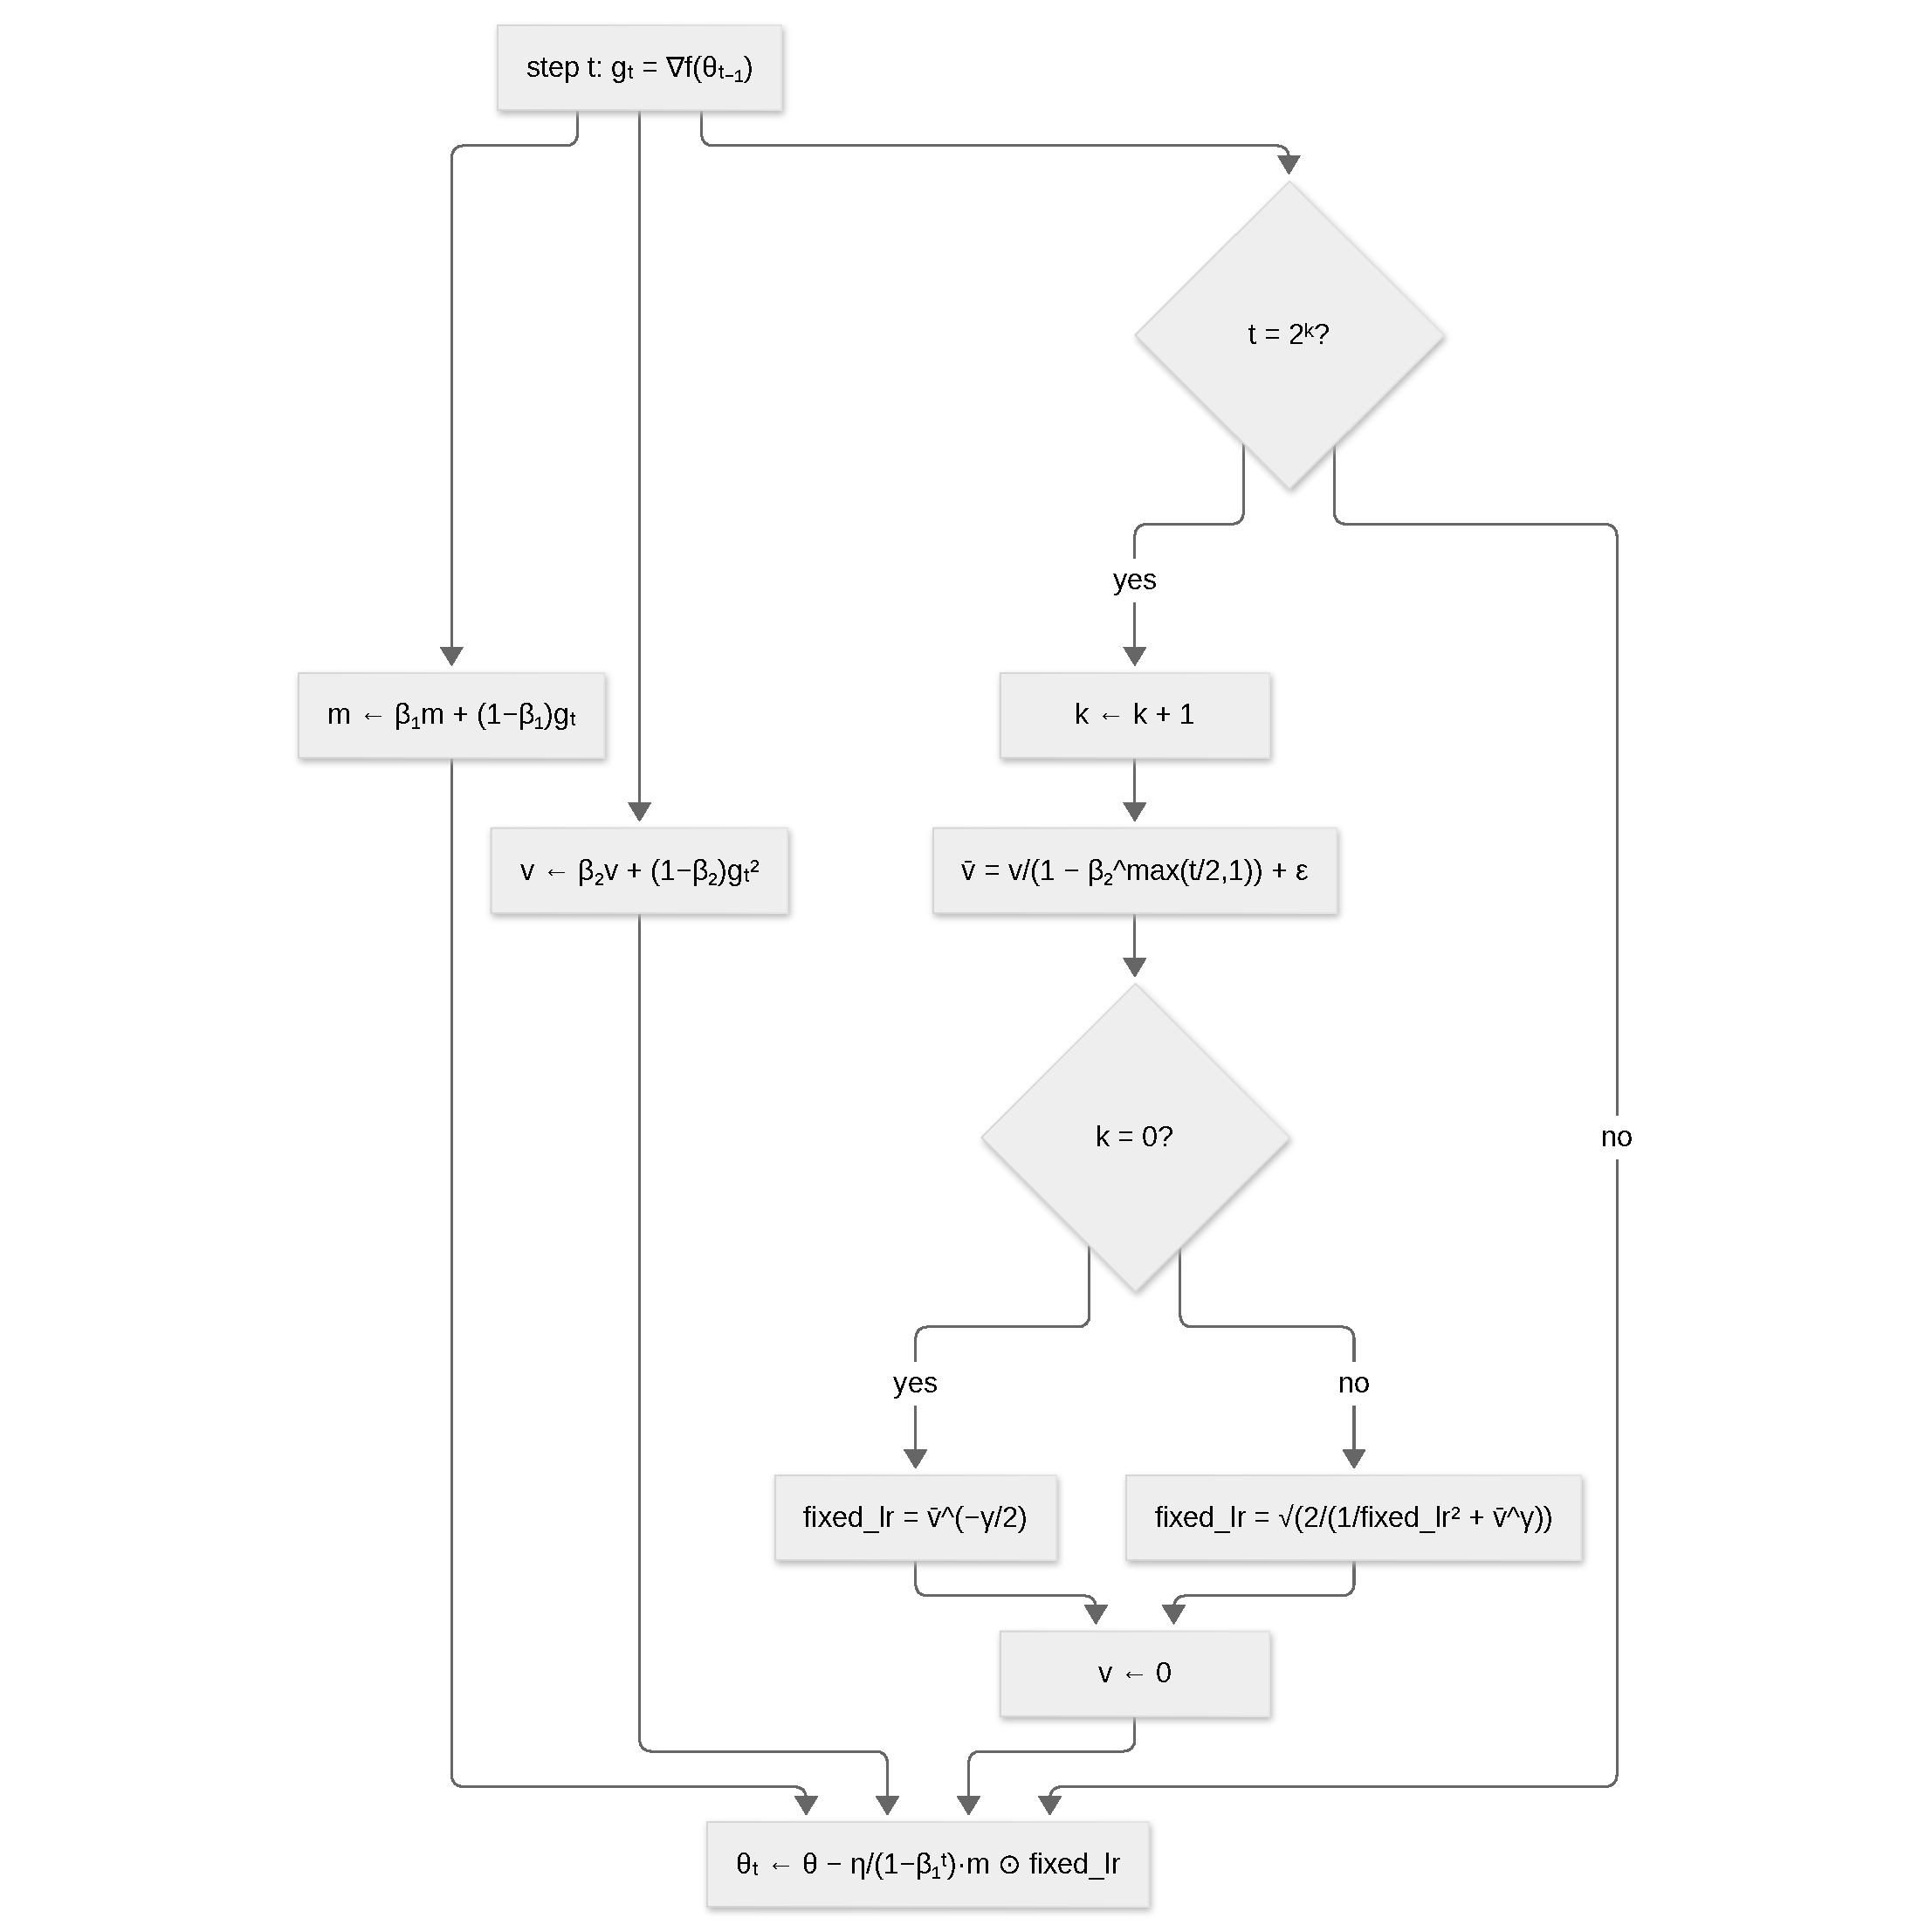
\includegraphics{../paper/figures/optimizers/anon.pdf}}
\caption{Flujo por paso de Anon: el precondicionador IDU refrescado en potencias de dos, con adaptividad ajustable $\gamma$ y una actualización de momentum con corrección de sesgo.}
\label{fig:opt-anon}
\end{figure}
Anon \citep{anon2026anon} introduce adaptividad ajustable continuamente mediante un único parámetro $\gamma \in \mathbb{R}$, cerrando la brecha entre comportamientos tipo SGD ($\gamma=0$) y tipo Adam ($\gamma=1$), y extrapolando más allá de ambos. La innovación central es el mecanismo Incremental Delay Update (IDU), que permite convergencia estable a través de todo el espectro de adaptividad de valores reales:

\begin{align}
m_t &= \beta_1 m_{t-1} + (1-\beta_1) g_t \quad\text{(momento de primer orden)}\\
v_t &= \beta_2 v_{t-1} + (1-\beta_2) g_t^2 \quad\text{(momento de segundo orden)}\\
\bar{v}_t &= \frac{v_t}{1-\beta_2^{\max(t,1)}} + \epsilon \quad\text{(momento de segundo orden con corrección de sesgo)}\\
\text{fixed\_lr}_k &= \begin{cases}
\bar{v}_k^{-\gamma/2} & \text{si } k = 0 \\
\sqrt{2 / \left(\frac{1}{\text{fixed\_lr}_{k-1}^2} + \bar{v}_k^\gamma\right)} & \text{si } k > 0
\end{cases}\\
\theta_{t+1} &= \theta_t - \frac{\eta}{1-\beta_1^t} \cdot m_t \odot \text{fixed\_lr}_{\lfloor\log_2 t\rfloor}
\end{align}

A diferencia de los optimizadores adaptativos estándar, IDU actualiza el precondicionador solo en potencias de dos ($t = 2^k$), acumulando estadísticas de gradiente entre actualizaciones y agregándolas recursivamente. Este acumulador suave y multiescala evita el seguimiento estricto del máximo de AMSGrad mientras estabiliza demostrablemente la convergencia para cualquier $\gamma \in \mathbb{R}$. El parámetro $\gamma$ controla directamente la adaptividad: $\gamma > 1$ acelera la salida de puntos de silla (favorable para arquitecturas complejas), $\gamma = 1$ recupera el comportamiento tipo Adam, $\gamma = 0$ produce escalado tipo SGD, y $\gamma < 0$ se sesga hacia mínimos más planos (beneficioso para arquitecturas clásicas como CNNs).

\begin{algorithm}[H]
\caption{Anon (Adaptivity Non-restricted Optimizer con IDU)}
\label{alg:anon}
\begin{algorithmic}[1]
\Require Parámetros iniciales $\theta_0$, tasa de aprendizaje $\eta$, $\beta_1, \beta_2$, tolerancia $\epsilon$, adaptividad $\gamma \in \mathbb{R}$
\Ensure Parámetros actualizados $\theta_T$
\State Inicializar: $m \gets 0$, $v \gets 0$, $fixed\_lr \gets 0$, paso $t \gets 0$, contador IDU $k \gets -1$
\For{$t = 1, 2, \ldots, T$}
    \State $g_t \gets \nabla f(\theta_{t-1})$
    \State $m \gets \beta_1 m + (1-\beta_1) g_t$
    \State $v \gets \beta_2 v + (1-\beta_2) g_t^2$
    \If{$t = 2^k$}
        \State $k \gets k+1$
        \State $\bar{v} \gets v/(1 - \beta_2^{\max(t/2,1)}) + \epsilon$
        \If{$k = 0$}
            \State fixed\_lr $\gets \bar{v}^{-\gamma/2}$
        \Else
            \State fixed\_lr $\gets \sqrt{2 / (1/\text{fixed\_lr}^2 + \bar{v}^\gamma)}$
        \EndIf
        \State $v \gets 0$
    \EndIf
    \State $\theta_t \gets \theta_{t-1} - \frac{\eta}{1-\beta_1^t} \cdot m \odot \text{fixed\_lr}$
\EndFor
\Return $\theta_T$
\end{algorithmic}
\end{algorithm}

\paragraph{Contras.}
\begin{itemize}[leftmargin=*]
\item Mantiene tres búferes de estado ($m$, $v$, fixed\_lr) y refresca el precondicionador con una programación logarítmica.
\item El parámetro de adaptividad $\gamma$ debe seleccionarse por arquitectura.
\end{itemize}

\paragraph{Ventajas.}
\begin{itemize}[leftmargin=*]
\item Misma clase de complejidad $\mathcal{O}(n)$ por paso que AdamW, con adaptividad ajustable de forma continua.
\item IDU alcanza demostrablemente regret $\mathcal{O}(\sqrt{T})$ para problemas convexos y $\mathcal{O}(\ln T/\sqrt{T})$ para entornos no convexos.
\end{itemize}

\paragraph{Prodigy (Approximating the Distance Estimate).}
\begin{figure}[H]
\centering
\fitfigure{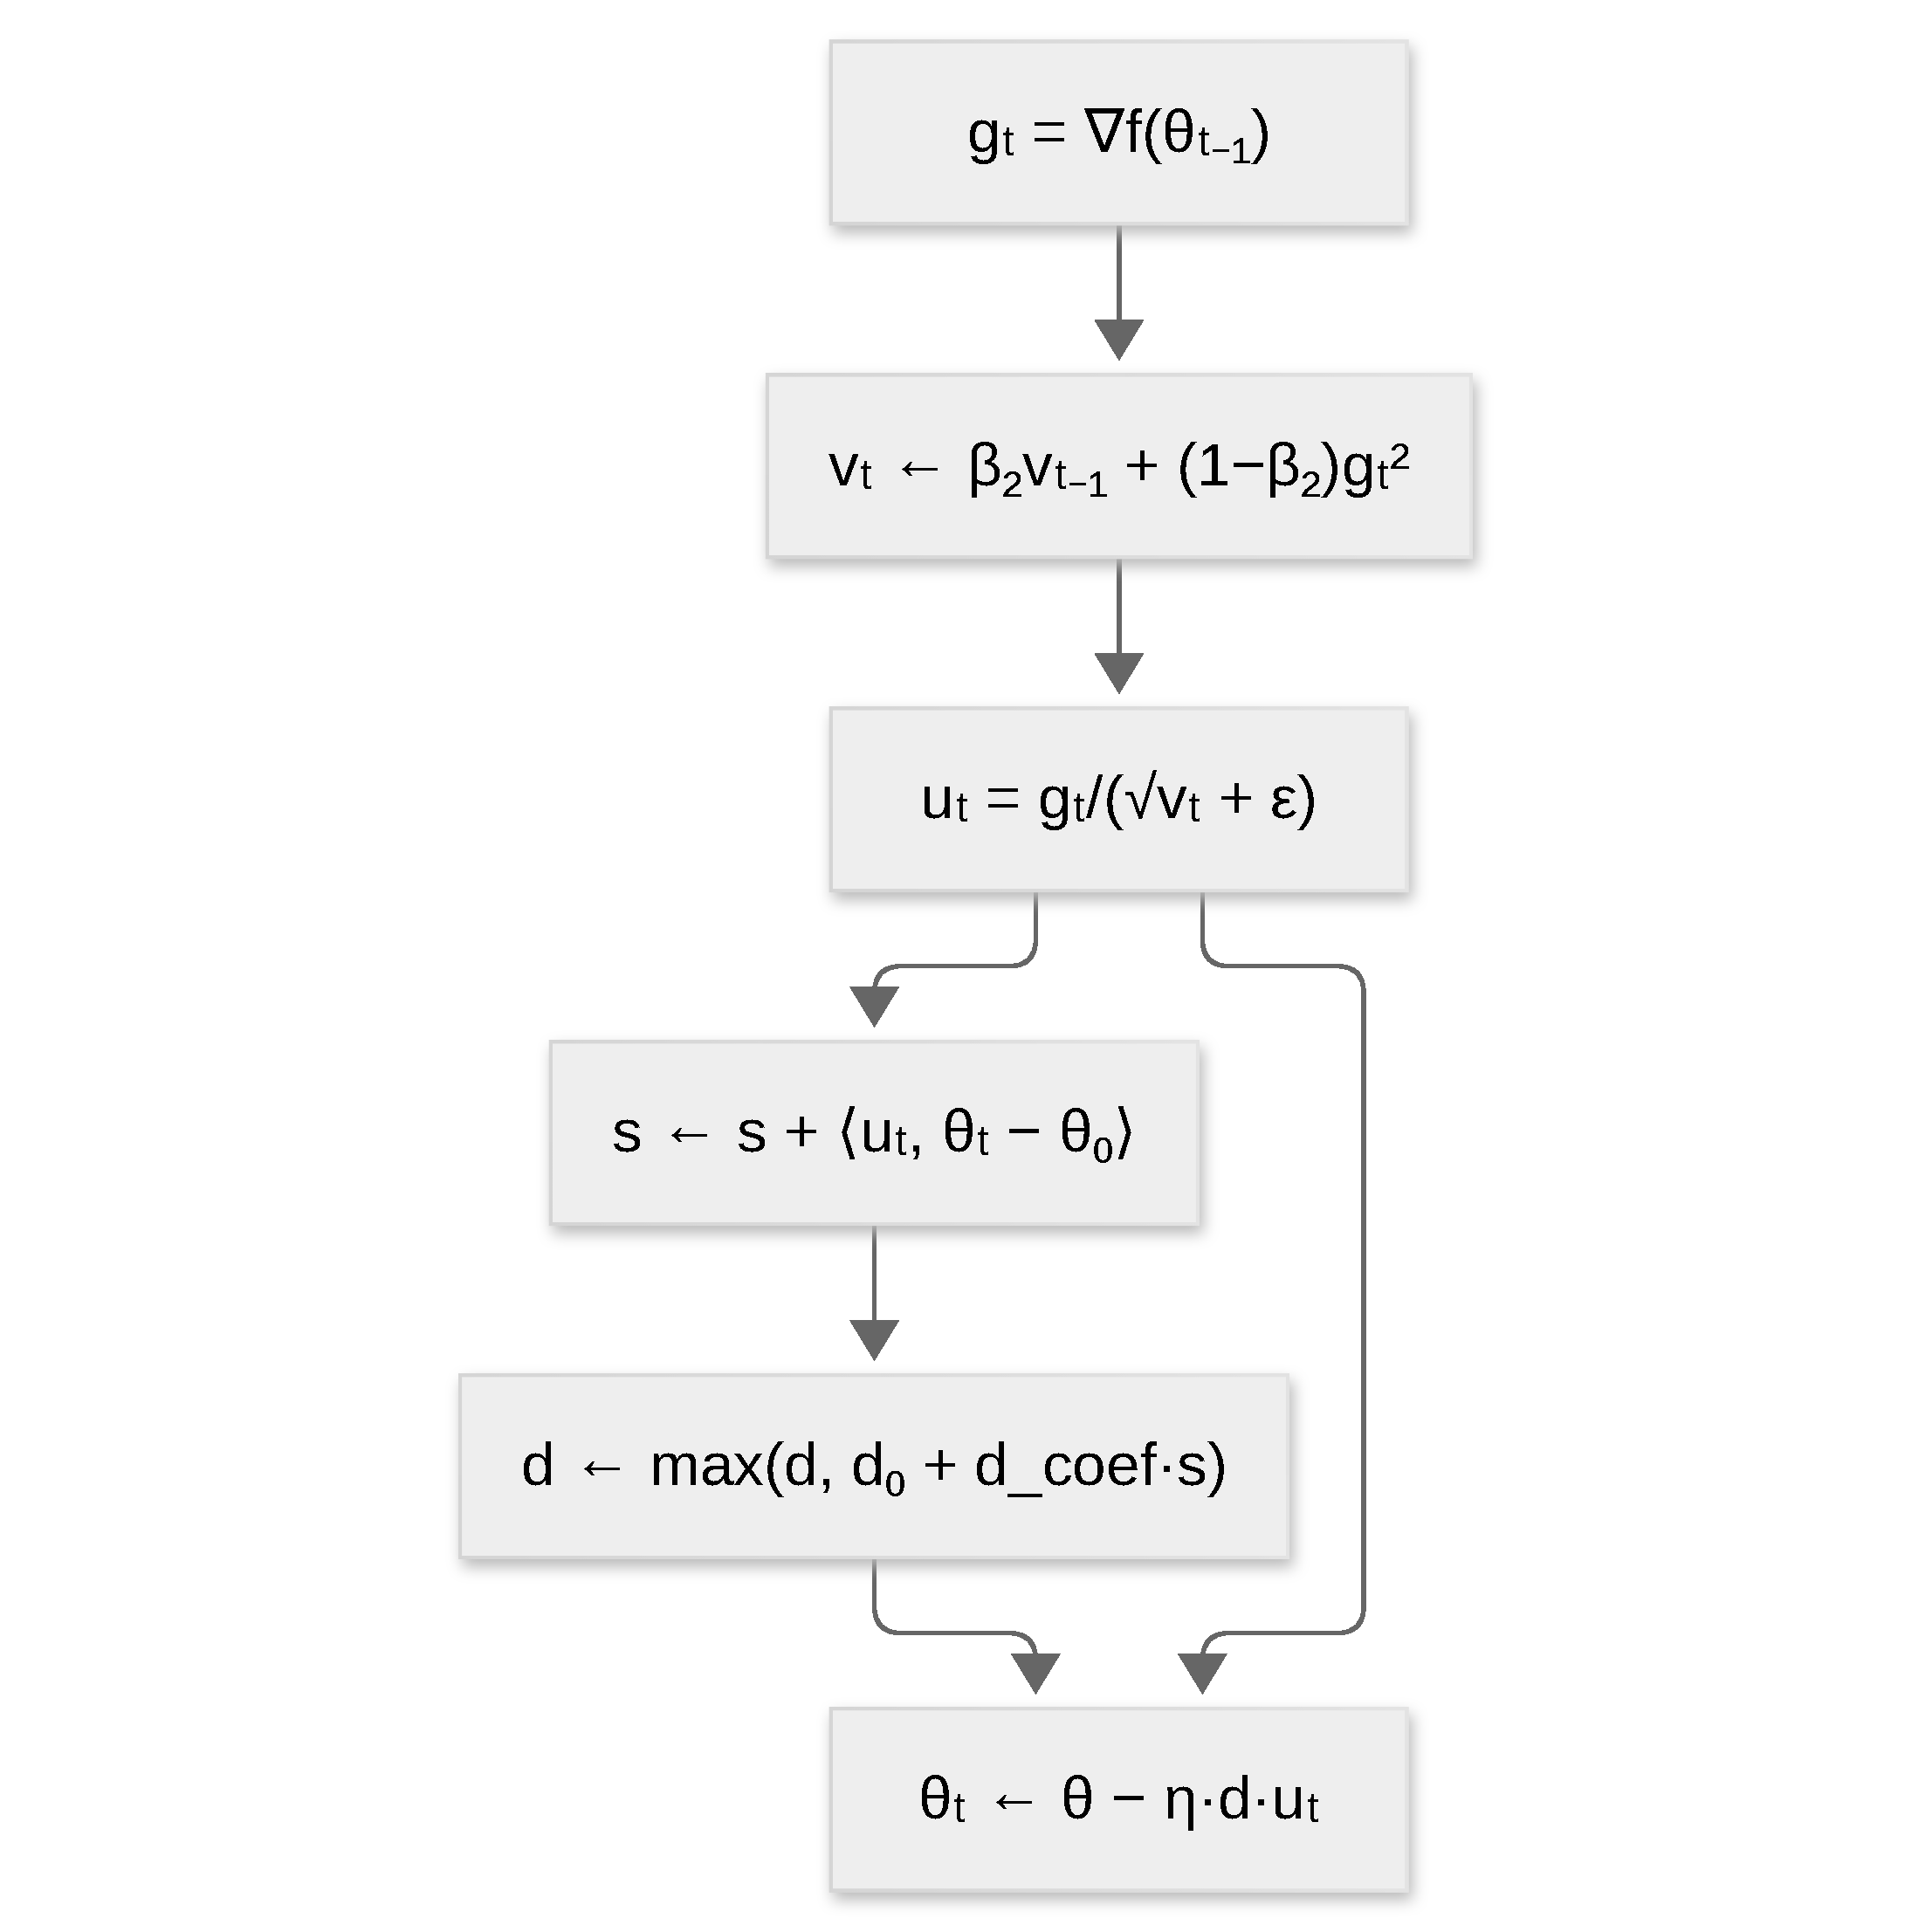
\includegraphics{../paper/figures/optimizers/prodigy.pdf}}
\caption{Flujo por paso de Prodigy: una estimación de distancia signada acumulativa que escala el paso adaptativo sin programación de tasa de aprendizaje.}
\label{fig:opt-prodigy}
\end{figure}
Prodigy adapta la escala efectiva del paso mediante una estadística tipo distancia acumulativa, eliminando la necesidad de ajuste explícito de la tasa de aprendizaje. El algoritmo mantiene una estimación de distancia acumulativa:
\begin{align}
u_t &= \frac{g_t}{\sqrt{v_t}+\epsilon} \quad\text{(paso adaptativo no normalizado)} \\
s_t &= s_{t-1} + \langle u_t, \theta_t - \theta_0 \rangle \quad\text{(distancia signada acumulativa)} \\
d_t &= \max(d_{t-1}, d_0 + d_{\text{coef}} \cdot s_t) \quad\text{(estimación de distancia con cota inferior)} \\
\theta_{t+1} &= \theta_t - \eta \cdot d_t \cdot u_t
\end{align}
donde $d_0$ es una cota inicial y $d_{\text{coef}}$ controla qué tan agresivamente se adapta la estimación. La estimación de distancia $d_t$ captura la magnitud combinada de gradientes pasados ponderada por el desplazamiento real de los parámetros, implementando una tasa de aprendizaje efectiva implícita.

\begin{algorithm}[H]
\caption{Prodigy (Approximating the Distance Estimate)}
\label{alg:prodigy}
\begin{algorithmic}[1]
\Require Parámetros iniciales $\theta_0$, tasa de aprendizaje $\eta$, coeficiente $d_{\text{coef}}$, distancia inicial $d_0 > 0$
\Ensure Parámetros actualizados $\theta_T$
\State Inicializar: $s \gets 0$ (distancia signada acumulativa), $d \gets d_0$
\For{$t = 1, 2, \ldots, T$}
    \State $g_t \gets \nabla f(\theta_{t-1})$
    \State $v_t \gets \beta_2 v_{t-1} + (1-\beta_2) g_t^2$ \Comment{Segundo momento}
    \State $u_t \gets g_t / (\sqrt{v_t} + \epsilon)$ \Comment{Adaptativo no normalizado}
    \State Actualizar distancia: $s \gets s + \langle u_t, \theta_t - \theta_0 \rangle$ \Comment{Distancia signada}
    \State $d \gets \max(d, d_0 + d_{\text{coef}} \cdot s)$ \Comment{Distancia con cota inferior}
    \State $\theta_t \gets \theta_{t-1} - \eta \cdot d \cdot u_t$ \Comment{Actualización escalada por distancia}
\EndFor
\Return $\theta_T$
\end{algorithmic}
\end{algorithm}

\paragraph{Contras.}
\begin{itemize}[leftmargin=*]
\item Introduce los hiperparámetros $d_0$ y $d_{\text{coef}}$ para la estimación de distancia.
\item Añade un paso de contabilidad de producto interno por iteración.
\end{itemize}

\paragraph{Ventajas.}
\begin{itemize}[leftmargin=*]
\item Elimina el ajuste y la programación explícitos de la tasa de aprendizaje.
\item Convergencia robusta en distintas escalas de problemas y tamaños de lote.
\end{itemize}

\subsection{Optimizadores de Segundo Orden, Geométricos y de Ortogonalidad}
\paragraph{Shampoo (Precondicionamiento Matricial mediante Productos de Kronecker).}
\begin{figure}[H]
\centering
\fitfigure{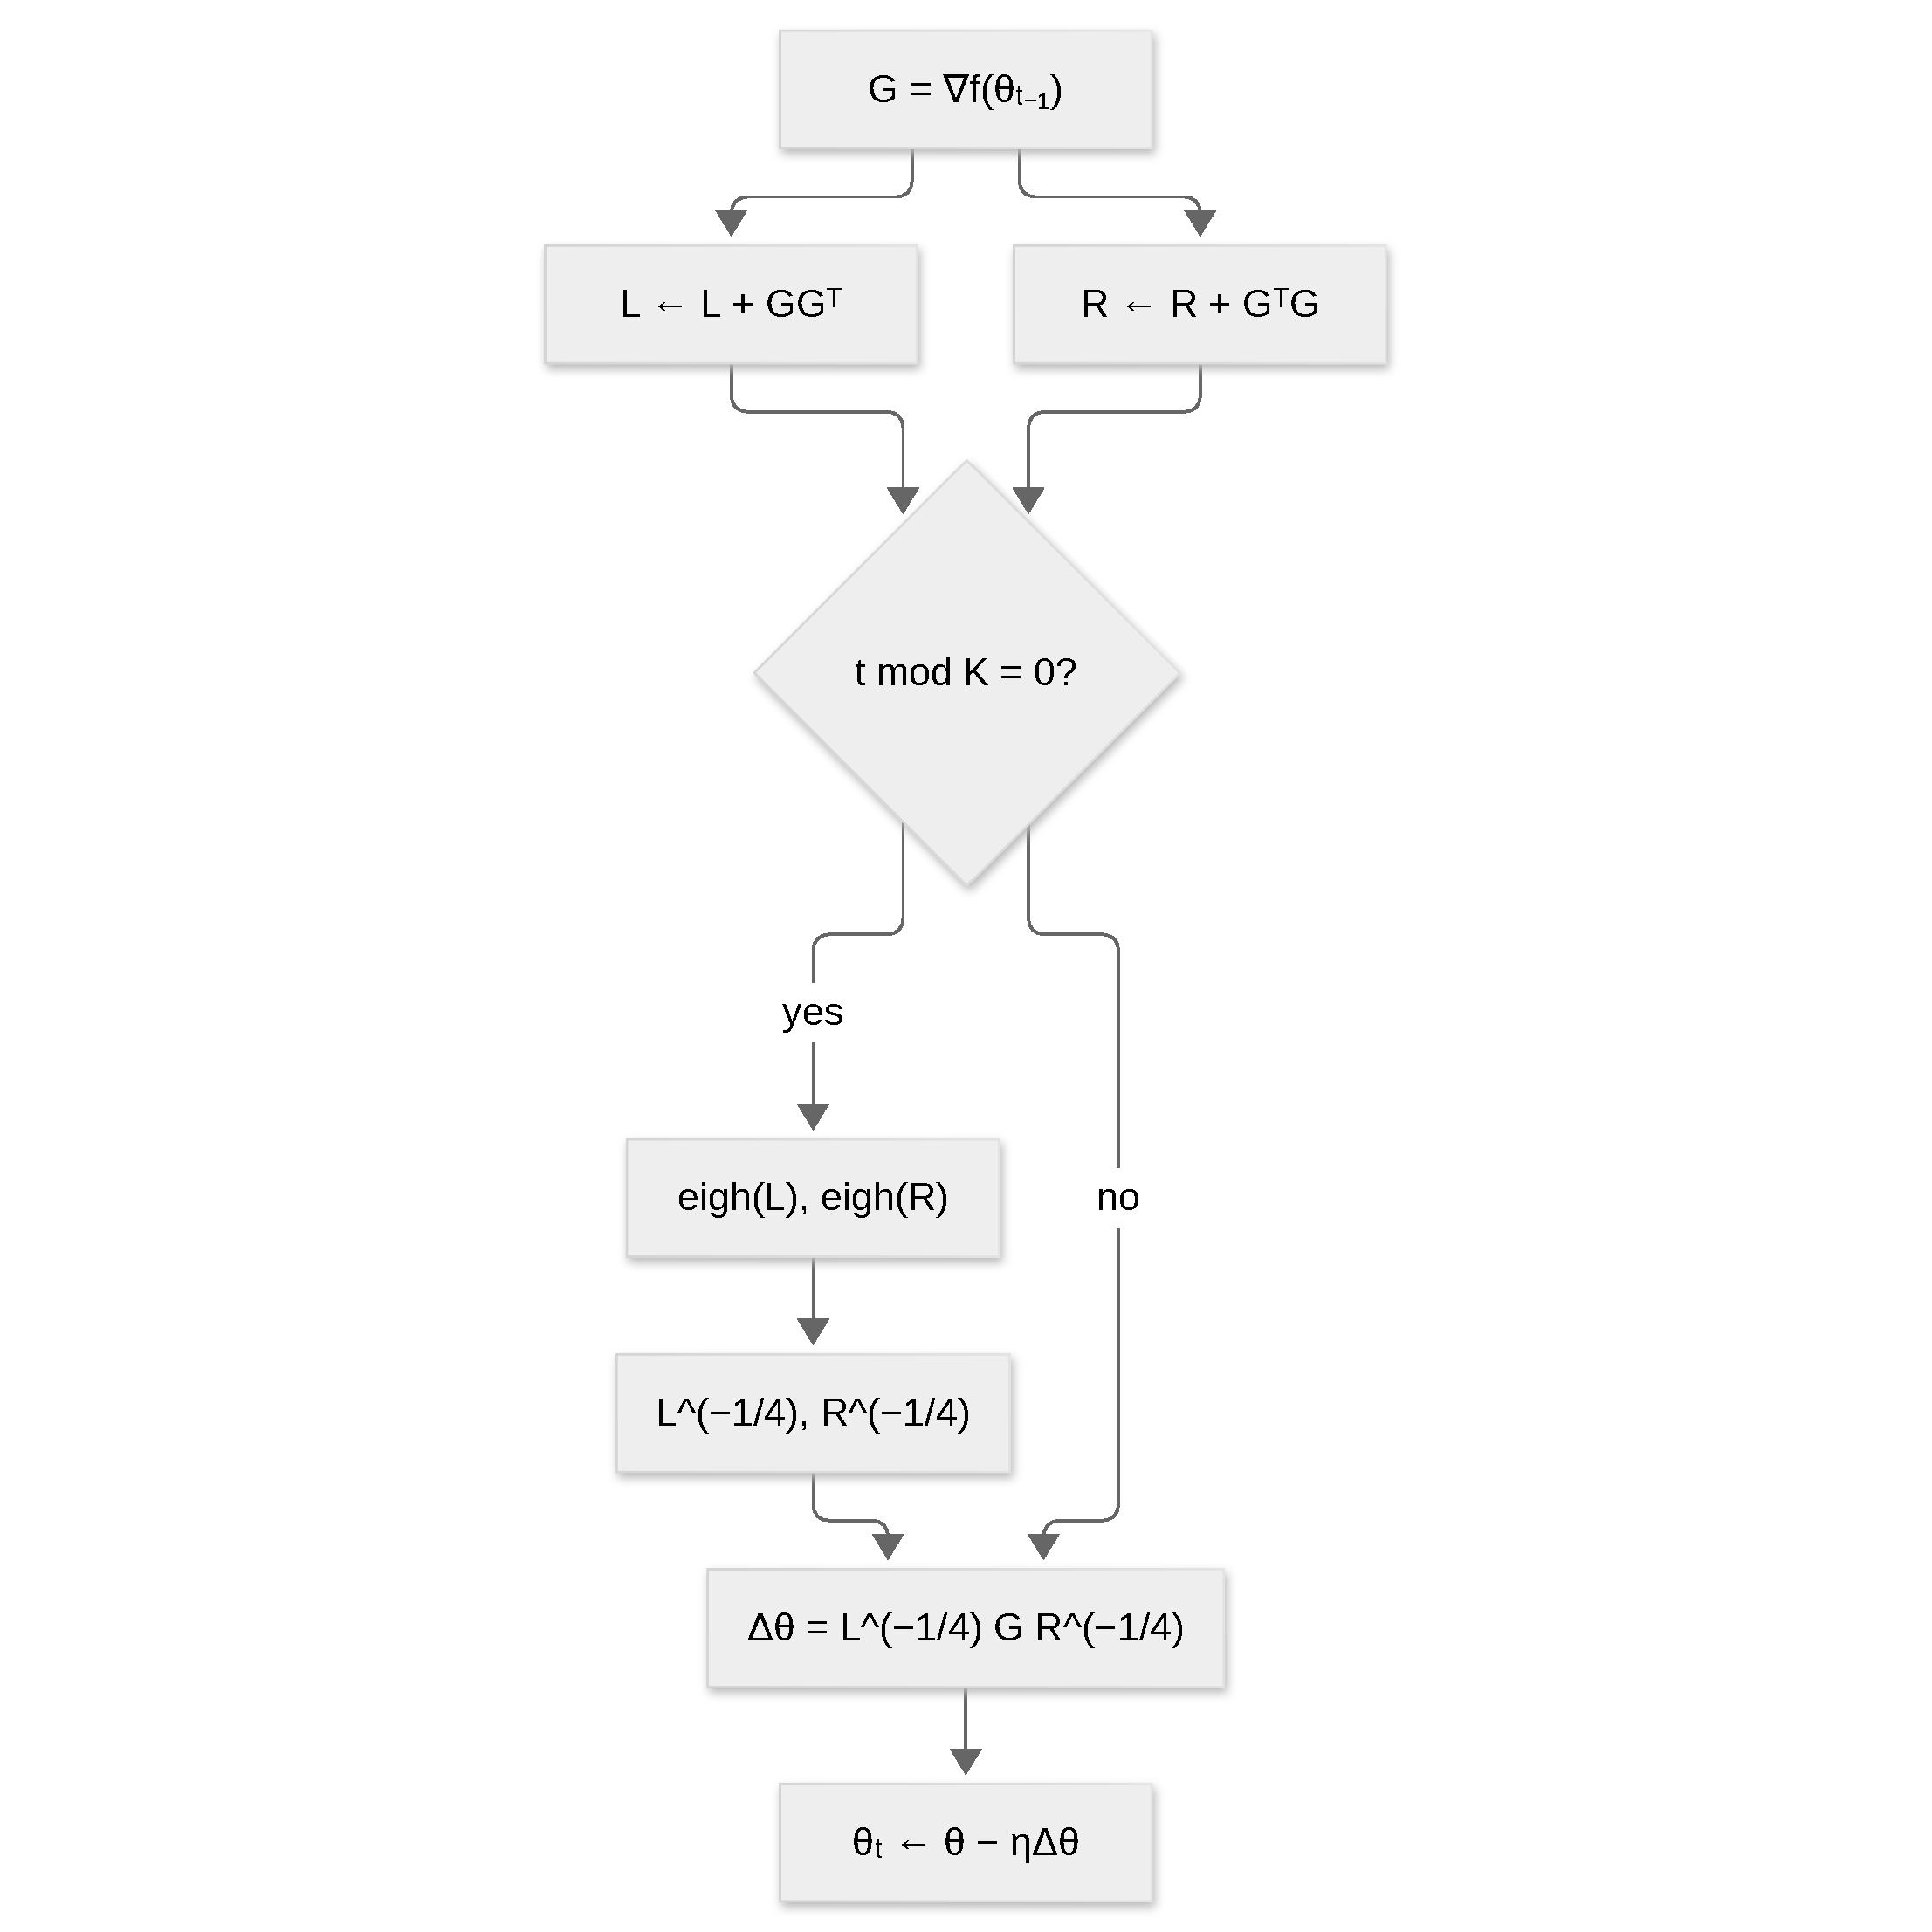
\includegraphics{../paper/figures/optimizers/shampoo.pdf}}
\caption{Flujo por paso de Shampoo: matrices de Gram factorizadas por Kronecker, eigendescomposición periódica y precondicionamiento del gradiente con raíz cuarta.}
\label{fig:opt-shampoo}
\end{figure}
Shampoo es un \textbf{método estructurado de segundo orden} que calcula precondicionadores matriciales a partir de estadísticas de producto exterior con estructura de Kronecker. Para una matriz de parámetros 2D $W \in \mathbb{R}^{m \times n}$:
\begin{align}
L_t &= L_{t-1} + G_t G_t^\top \quad\text{(matriz de Gram izquierda/filas, $m \times m$)} \\
R_t &= R_{t-1} + G_t^\top G_t \quad\text{(matriz de Gram derecha/columnas, $n \times n$)} \\
L_t^{-1/4} &= Q_L (\Lambda_L)^{-1/4} Q_L^\top \quad\text{(mediante eigendescomposición)} \\
R_t^{-1/4} &= Q_R (\Lambda_R)^{-1/4} Q_R^\top \\
\Delta W_t &= L_t^{-1/4} G_t R_t^{-1/4} \quad\text{(gradiente precondicionado)}
\end{align}
Shampoo aproxima el precondicionador de matriz completa de Adagrad $H^{-1/2}$ (donde $H$ es el Hessiano) utilizando estructura factorizada de Kronecker. En lugar de almacenar un precondicionador de $(mn) \times (mn)$, Shampoo mantiene dos matrices más pequeñas ($m \times m$ y $n \times n$), capturando correlaciones entre parámetros dentro y entre grupos. Las eigendescomposiciones se realizan periódicamente (e.g., cada $K=10$ pasos) para amortizar el costo.

\begin{algorithm}[H]
\caption{Shampoo (Precondicionamiento Matricial mediante Productos de Kronecker)}
\label{alg:shampoo}
\begin{algorithmic}[1]
\Require Parámetros iniciales $\theta_0$, tasa de aprendizaje $\eta$, intervalo de eigendescomposición $K$
\Ensure Parámetros actualizados $\theta_T$
\State Inicializar: $L \gets \epsilon I_m$, $R \gets \epsilon I_n$ (matrices de Gram izquierda y derecha)
\For{$t = 1, 2, \ldots, T$}
    \State $G \gets \nabla f(\theta_{t-1})$ \Comment{Gradiente}
    \State Actualizar matrices de Gram: $L \gets L + G G^\top$, $R \gets R + G^\top G$
    \If{$t \mod K == 0$}
        \State $Q_L, \Lambda_L \gets \text{eigh}(L)$ \Comment{Eigendescomposición de $L$}
        \State $Q_R, \Lambda_R \gets \text{eigh}(R)$ \Comment{Eigendescomposición de $R$}
        \State $L^{-1/4} \gets Q_L (\Lambda_L + \epsilon)^{-1/4} Q_L^\top$
        \State $R^{-1/4} \gets Q_R (\Lambda_R + \epsilon)^{-1/4} Q_R^\top$
    \EndIf
    \State $\Delta \theta \gets L^{-1/4} G R^{-1/4}$ \Comment{Gradiente precondicionado}
    \State $\theta_t \gets \theta_{t-1} - \eta \cdot \Delta \theta$
\EndFor
\Return $\theta_T$
\end{algorithmic}
\end{algorithm}

\paragraph{Contras.}
\begin{itemize}[leftmargin=*]
\item Eigendescomposiciones periódicas $O(m^3+n^3)$ y mayor cómputo por paso.
\item Asume estructura de parámetros 2D; los embeddings y sesgos requieren manejo aparte.
\end{itemize}

\paragraph{Ventajas.}
\begin{itemize}[leftmargin=*]
\item Precondicionamiento de segundo orden factorizado por Kronecker sin una matriz densa $(mn)\times(mn)$.
\item Demostrado efectivo a escala de producción y adecuado para matrices transformer de alto rango, con mejor condicionamiento y convergencia acelerada.
\end{itemize}

\paragraph{SOAP (Shampoo with Adam in eigenbasis).}
\begin{figure}[H]
\centering
\fitfigure{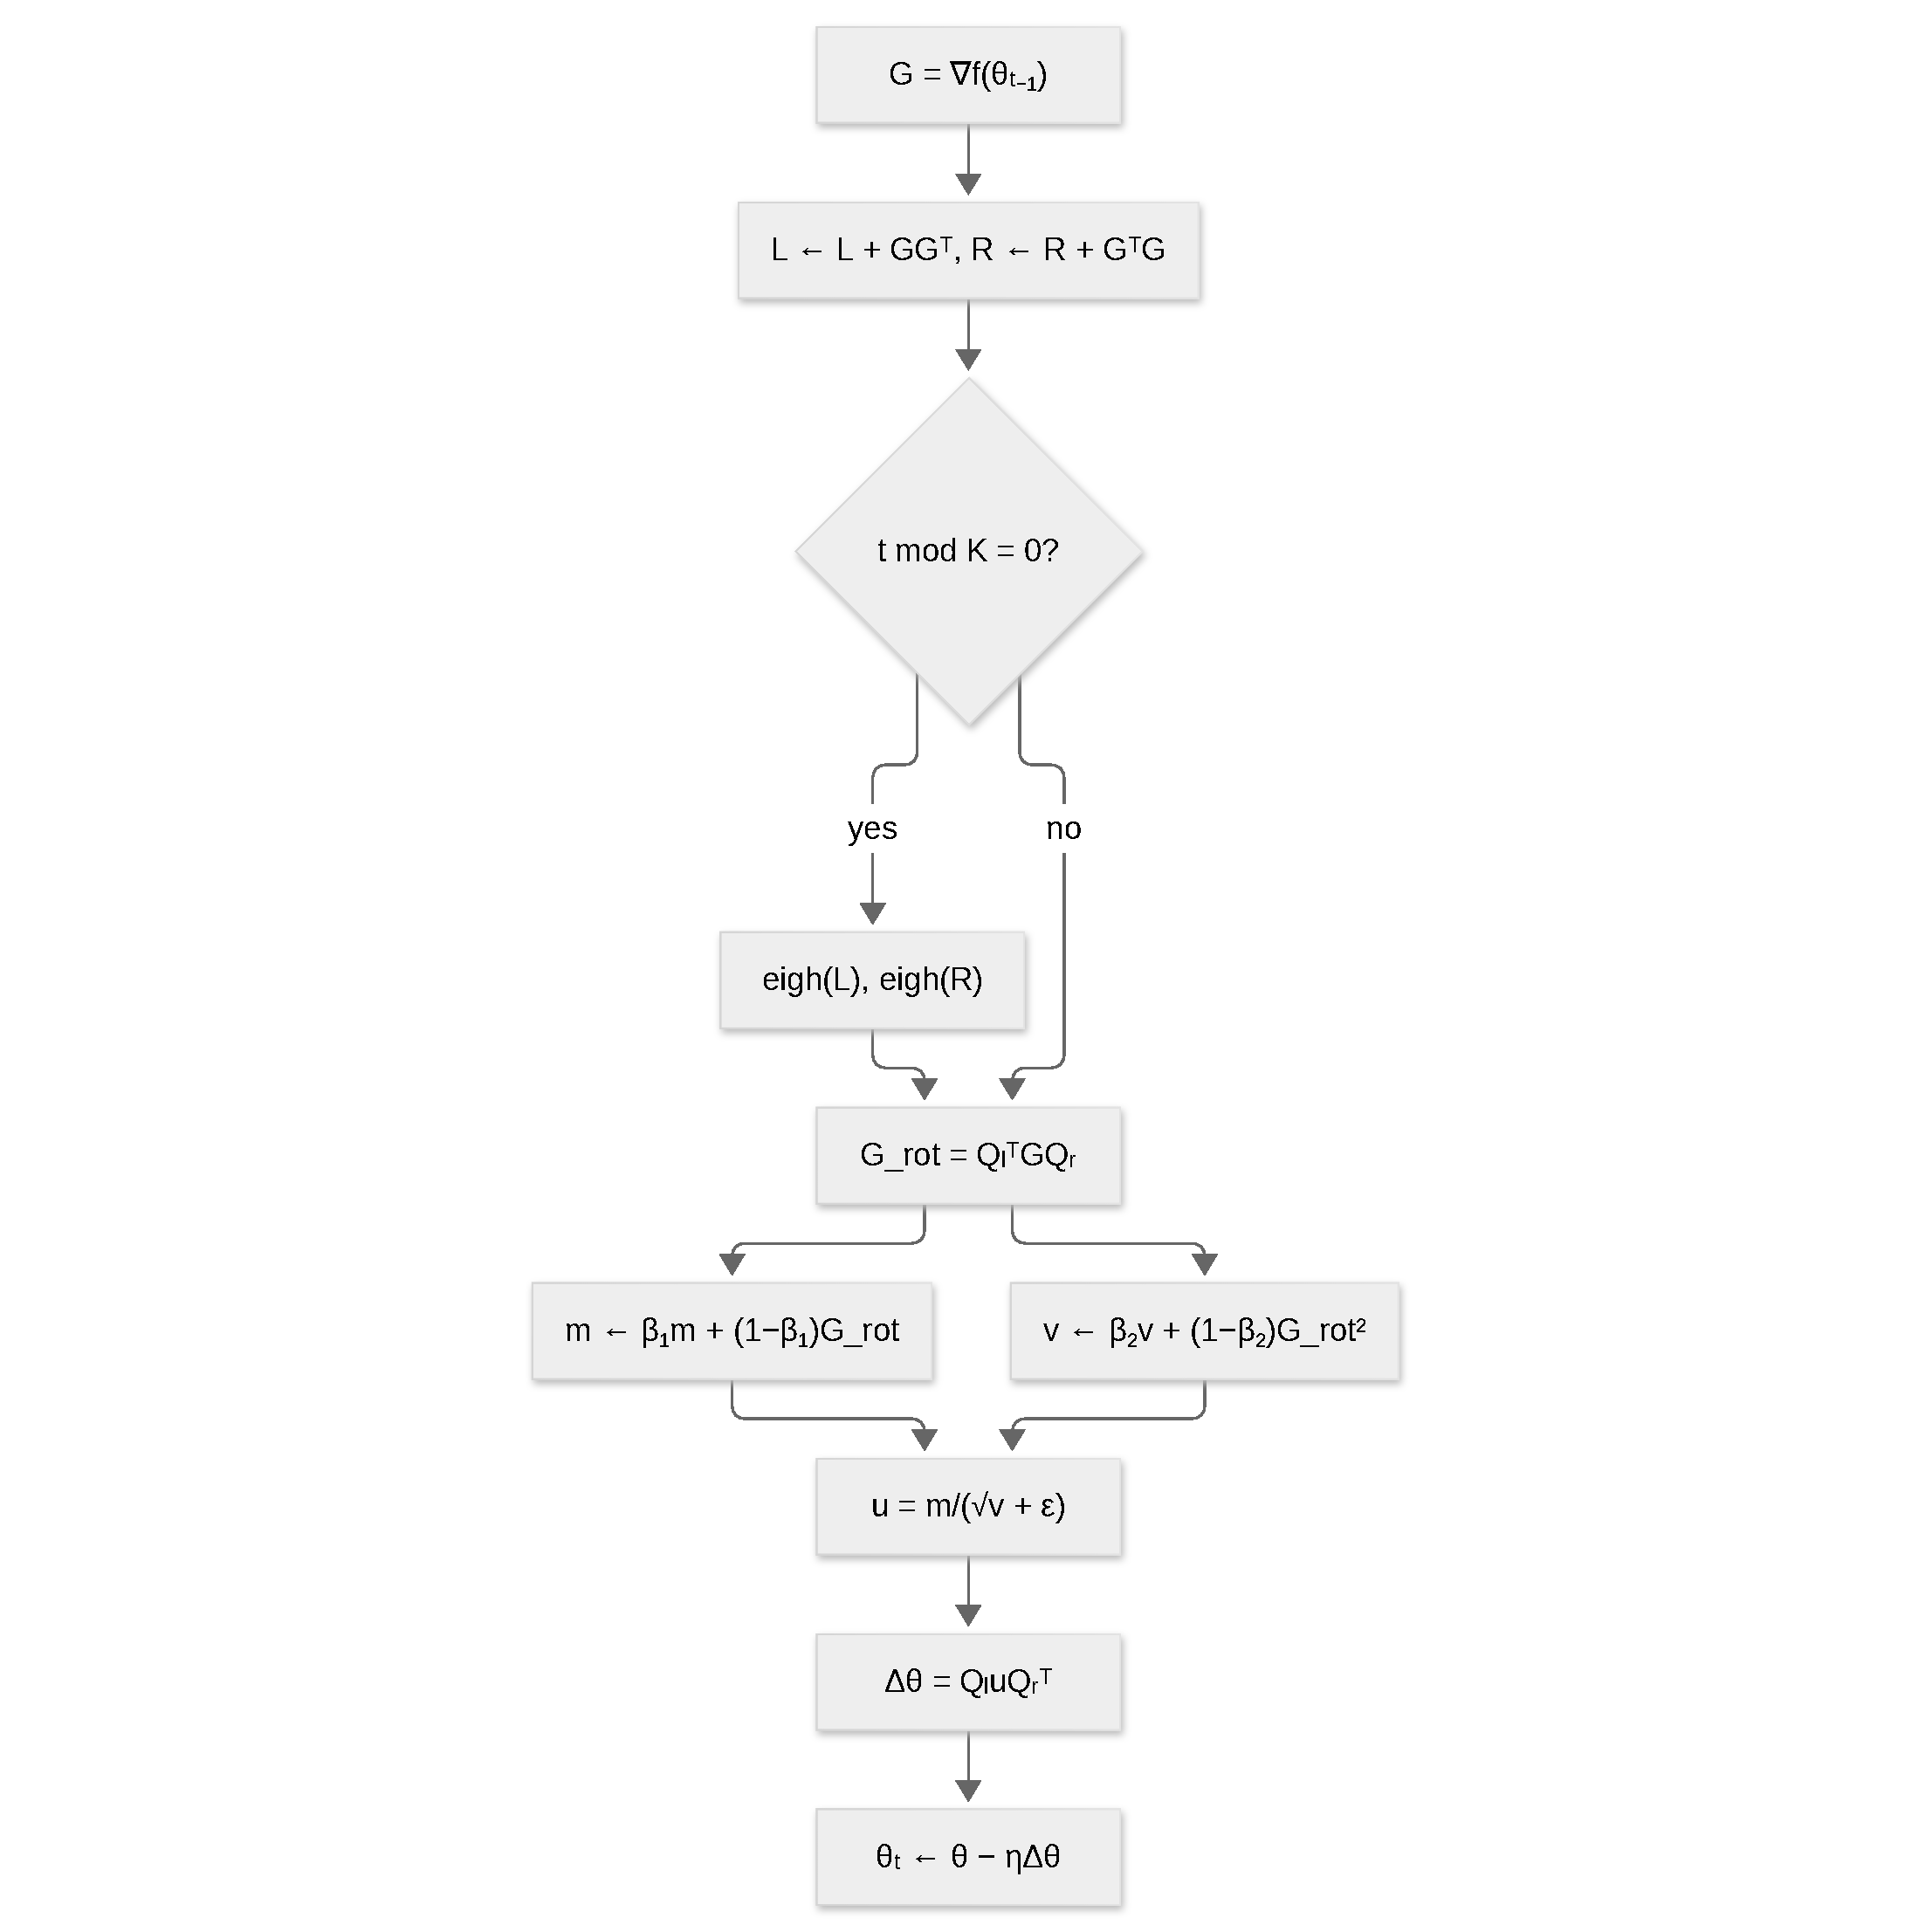
\includegraphics{../paper/figures/optimizers/soap.pdf}}
\caption{Flujo por paso de SOAP: momentos de Adam en la base de eigenvectores de Shampoo, rotados de vuelta al espacio de parámetros.}
\label{fig:opt-soap}
\end{figure}
SOAP es una variante simplificada de Shampoo que desacopla el precondicionamiento del seguimiento de momento. En lugar de álgebra matricial compleja sobre gradientes precondicionados, SOAP ejecuta Adam estándar en la base de eigenvectores de los precondicionadores de Shampoo:
\begin{align}
L_t &= L_{t-1} + G_t G_t^\top, \quad R_t = R_{t-1} + G_t^\top G_t \quad\text{(acumulación de Gram)} \\
Q_L, \Lambda_L &= \text{eigh}(L_t), \quad Q_R, \Lambda_R = \text{eigh}(R_t) \quad\text{(eigendescomposición periódica)} \\
G_t^{\text{rot}} &= Q_L^\top G_t Q_R \quad\text{(rotar gradiente a la base de eigenvectores)} \\
m_t^{\text{rot}} &= \beta_1 m_{t-1}^{\text{rot}} + (1-\beta_1) G_t^{\text{rot}} \\
v_t^{\text{rot}} &= \beta_2 v_{t-1}^{\text{rot}} + (1-\beta_2)(G_t^{\text{rot}})^2 \quad\text{(Adam en el espacio rotado)} \\
U_t^{\text{rot}} &= \frac{m_t^{\text{rot}}}{\sqrt{v_t^{\text{rot}}}+\epsilon}, \quad U_t = Q_L U_t^{\text{rot}} Q_R^\top \quad\text{(rotar de vuelta)}
\end{align}
La idea clave: todo el seguimiento de momento ocurre en la base de eigenvectores bien condicionada, simplificando la estabilidad numérica y el análisis teórico.

\begin{algorithm}[H]
\caption{SOAP (Shampoo with Adam in Eigenbasis)}
\label{alg:soap}
\begin{algorithmic}[1]
\Require Parámetros iniciales $\theta_0$, tasa de aprendizaje $\eta$, $\beta_1, \beta_2$, intervalo de eigendescomposición $K$
\Ensure Parámetros actualizados $\theta_T$
\State Inicializar: $L \gets \epsilon I_m$, $R \gets \epsilon I_n$, $m \gets 0$, $v \gets 0$
\For{$t = 1, 2, \ldots, T$}
    \State $G \gets \nabla f(\theta_{t-1})$ \Comment{Gradiente}
    \State Actualizar Gram: $L \gets L + G G^\top$, $R \gets R + G^\top G$
    \If{$t \mod K == 0$}
        \State $Q_L, \Lambda_L \gets \text{eigh}(L)$, $Q_R, \Lambda_R \gets \text{eigh}(R)$
    \EndIf
    \State $G^{\text{rot}} \gets Q_L^\top G Q_R$ \Comment{Rotar gradiente a la base de eigenvectores}
    \State $m \gets \beta_1 m + (1-\beta_1) G^{\text{rot}}$ \Comment{Media móvil exponencial (corregir sesgo externamente)}
    \State $v \gets \beta_2 v + (1-\beta_2) (G^{\text{rot}})^2$ \Comment{Segundo momento (corregir sesgo externamente)}
    \State $u \gets m / (\sqrt{v} + \epsilon)$ \Comment{Paso adaptativo en la base de eigenvectores}
    \State $\Delta \theta \gets Q_L u Q_R^\top$ \Comment{Rotar de vuelta al espacio de parámetros}
    \State $\theta_t \gets \theta_{t-1} - \eta \cdot \Delta \theta$
\EndFor
\Return $\theta_T$
\end{algorithmic}
\end{algorithm}

\paragraph{Contras.}
\begin{itemize}[leftmargin=*]
\item Hereda el costo de eigendescomposición periódica de Shampoo.
\item La rotación y la rotación inversa añaden multiplicaciones de matrices por paso.
\end{itemize}

\paragraph{Ventajas.}
\begin{itemize}[leftmargin=*]
\item Combina la estructura de curvatura explícita de Shampoo con la mecánica de momentum probada de Adam.
\item A menudo más limpio y estable que Shampoo completo, con eigendescomposiciones amortizadas cada $K$ pasos.
\end{itemize}

\paragraph{Lion (EvoLved Sign Momentum).}
\begin{figure}[H]
\centering
\fitfigure{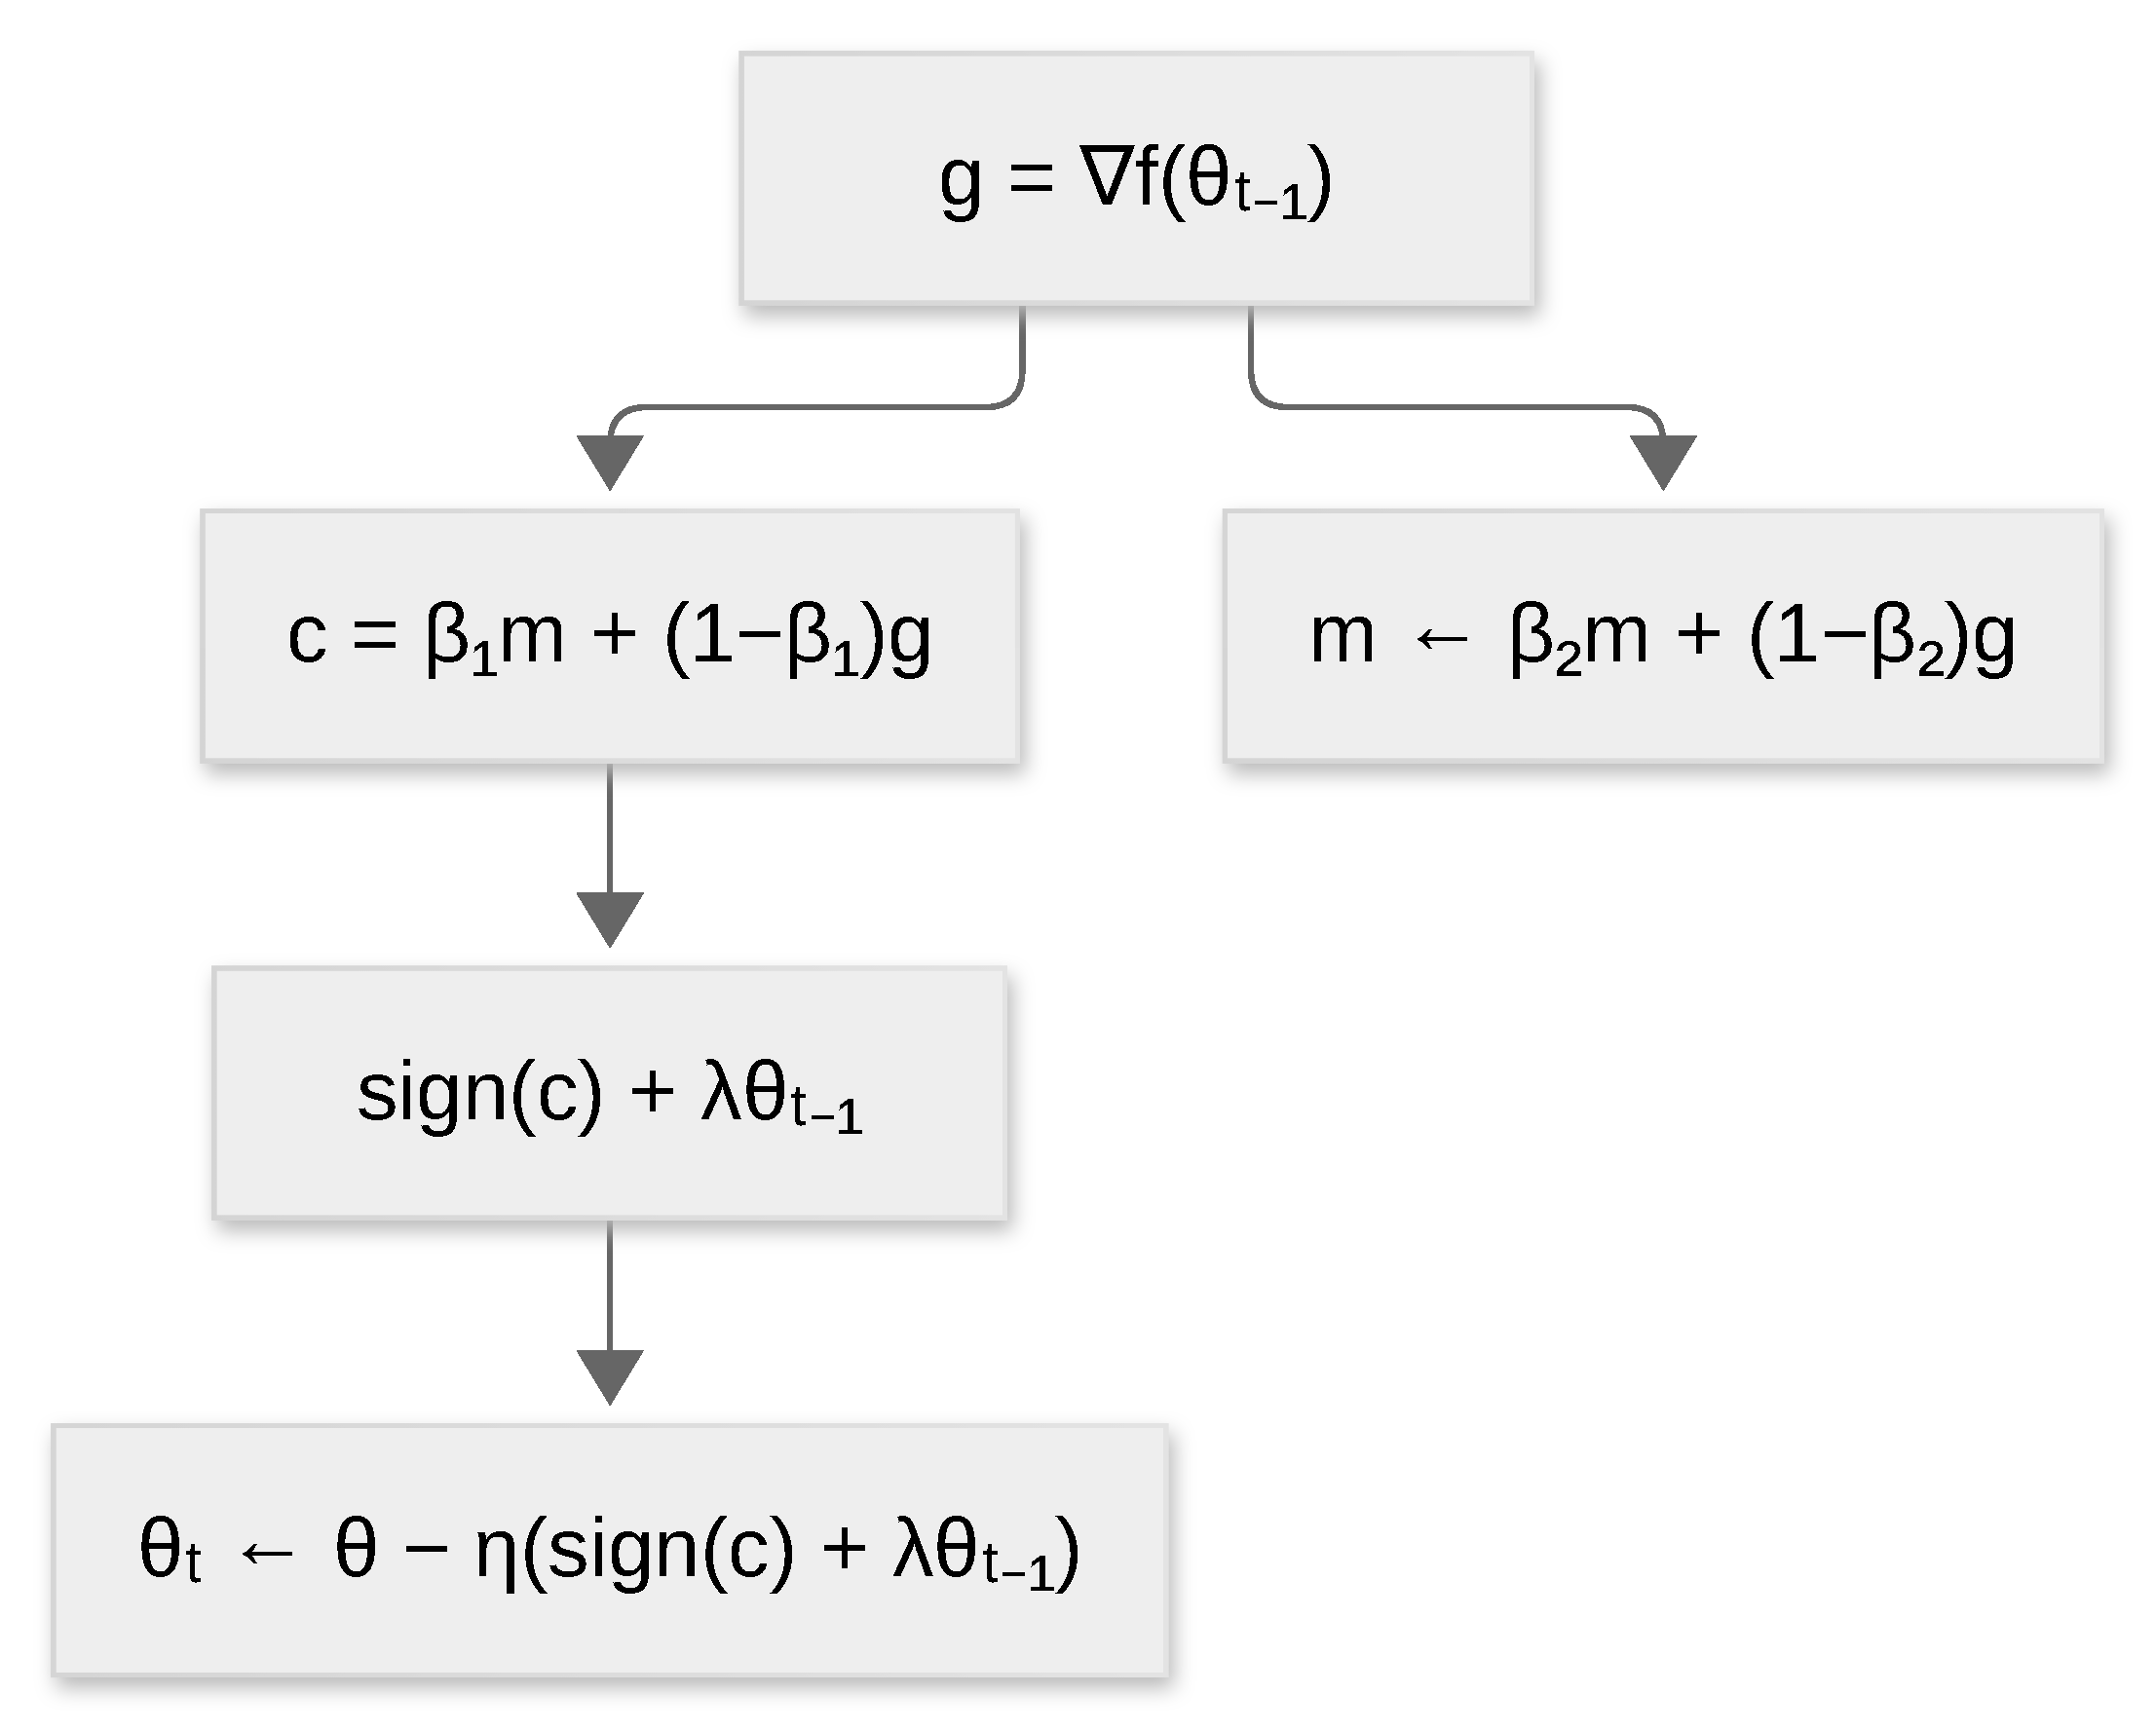
\includegraphics{../paper/figures/optimizers/lion.pdf}}
\caption{Flujo por paso de Lion: actualización por signo del momentum con acumulación de momentum desacoplada y decaimiento de pesos.}
\label{fig:opt-lion}
\end{figure}
Lion logra una \textbf{sobrecarga de memoria mínima} al usar actualizaciones basadas en signo en lugar de escalado adaptativo completo:
\begin{align}
c_t &= \beta_1 m_t + (1-\beta_1) g_t \quad\text{(entrada de momento)} \\
\theta_{t+1} &= \theta_t - \eta \left(\text{sign}(c_t) + \lambda\theta_t\right) \quad\text{(actualización con operador signo)} \\
m_{t+1} &= \beta_2 m_t + (1-\beta_2) g_t \quad\text{(acumulación de momento)}
\end{align}
Todas las operaciones de escalado elemento a elemento se reemplazan con \texttt{sign()}, que produce $\{-1, 0, +1\}$. Esto reduce drásticamente la memoria en comparación con métodos tipo Adam: Lion almacena solo el búfer de momento, sin varianza de segundo momento.

\begin{algorithm}[H]
\caption{Lion (EvoLved Sign Momentum)}
\label{alg:lion}
\begin{algorithmic}[1]
\Require Parámetros iniciales $\theta_0$, tasa de aprendizaje $\eta$, $\beta_1, \beta_2$, decaimiento de pesos $\lambda$
\Ensure Parámetros actualizados $\theta_T$
\State Inicializar: $m \gets 0$ (búfer de momento)
\For{$t = 1, 2, \ldots, T$}
    \State $g \gets \nabla f(\theta_{t-1})$ \Comment{Gradiente}
    \State $c \gets \beta_1 m + (1-\beta_1) g$ \Comment{Entrada de momento}
    \State $\theta_t \gets \theta_{t-1} - \eta (\text{sign}(c) + \lambda \theta_{t-1})$ \Comment{Actualización basada en signo con decaimiento de pesos}
    \State $m \gets \beta_2 m + (1-\beta_2) g$ \Comment{Acumulación de momento (desacoplada)}
\EndFor
\Return $\theta_T$
\end{algorithmic}
\end{algorithm}

\paragraph{Contras.}
\begin{itemize}[leftmargin=*]
\item Las actualizaciones por signo sacrifican la adaptación elemento a elemento de la tasa de aprendizaje que hace efectivo a Adam.
\item Puede ser menos robusto que los métodos de la familia Adam en tareas que requieren escalado adaptativo.
\end{itemize}

\paragraph{Ventajas.}
\begin{itemize}[leftmargin=*]
\item Almacena solo el búfer de momentum, sin varianza de segundo momento.
\item Opción de alto rendimiento y baja memoria para regímenes de lotes grandes donde domina la memoria de activaciones.
\end{itemize}

\paragraph{Sophia (Second-Order Hessian Information with Optimized Approximation).}
\begin{figure}[H]
\centering
\fitfigure{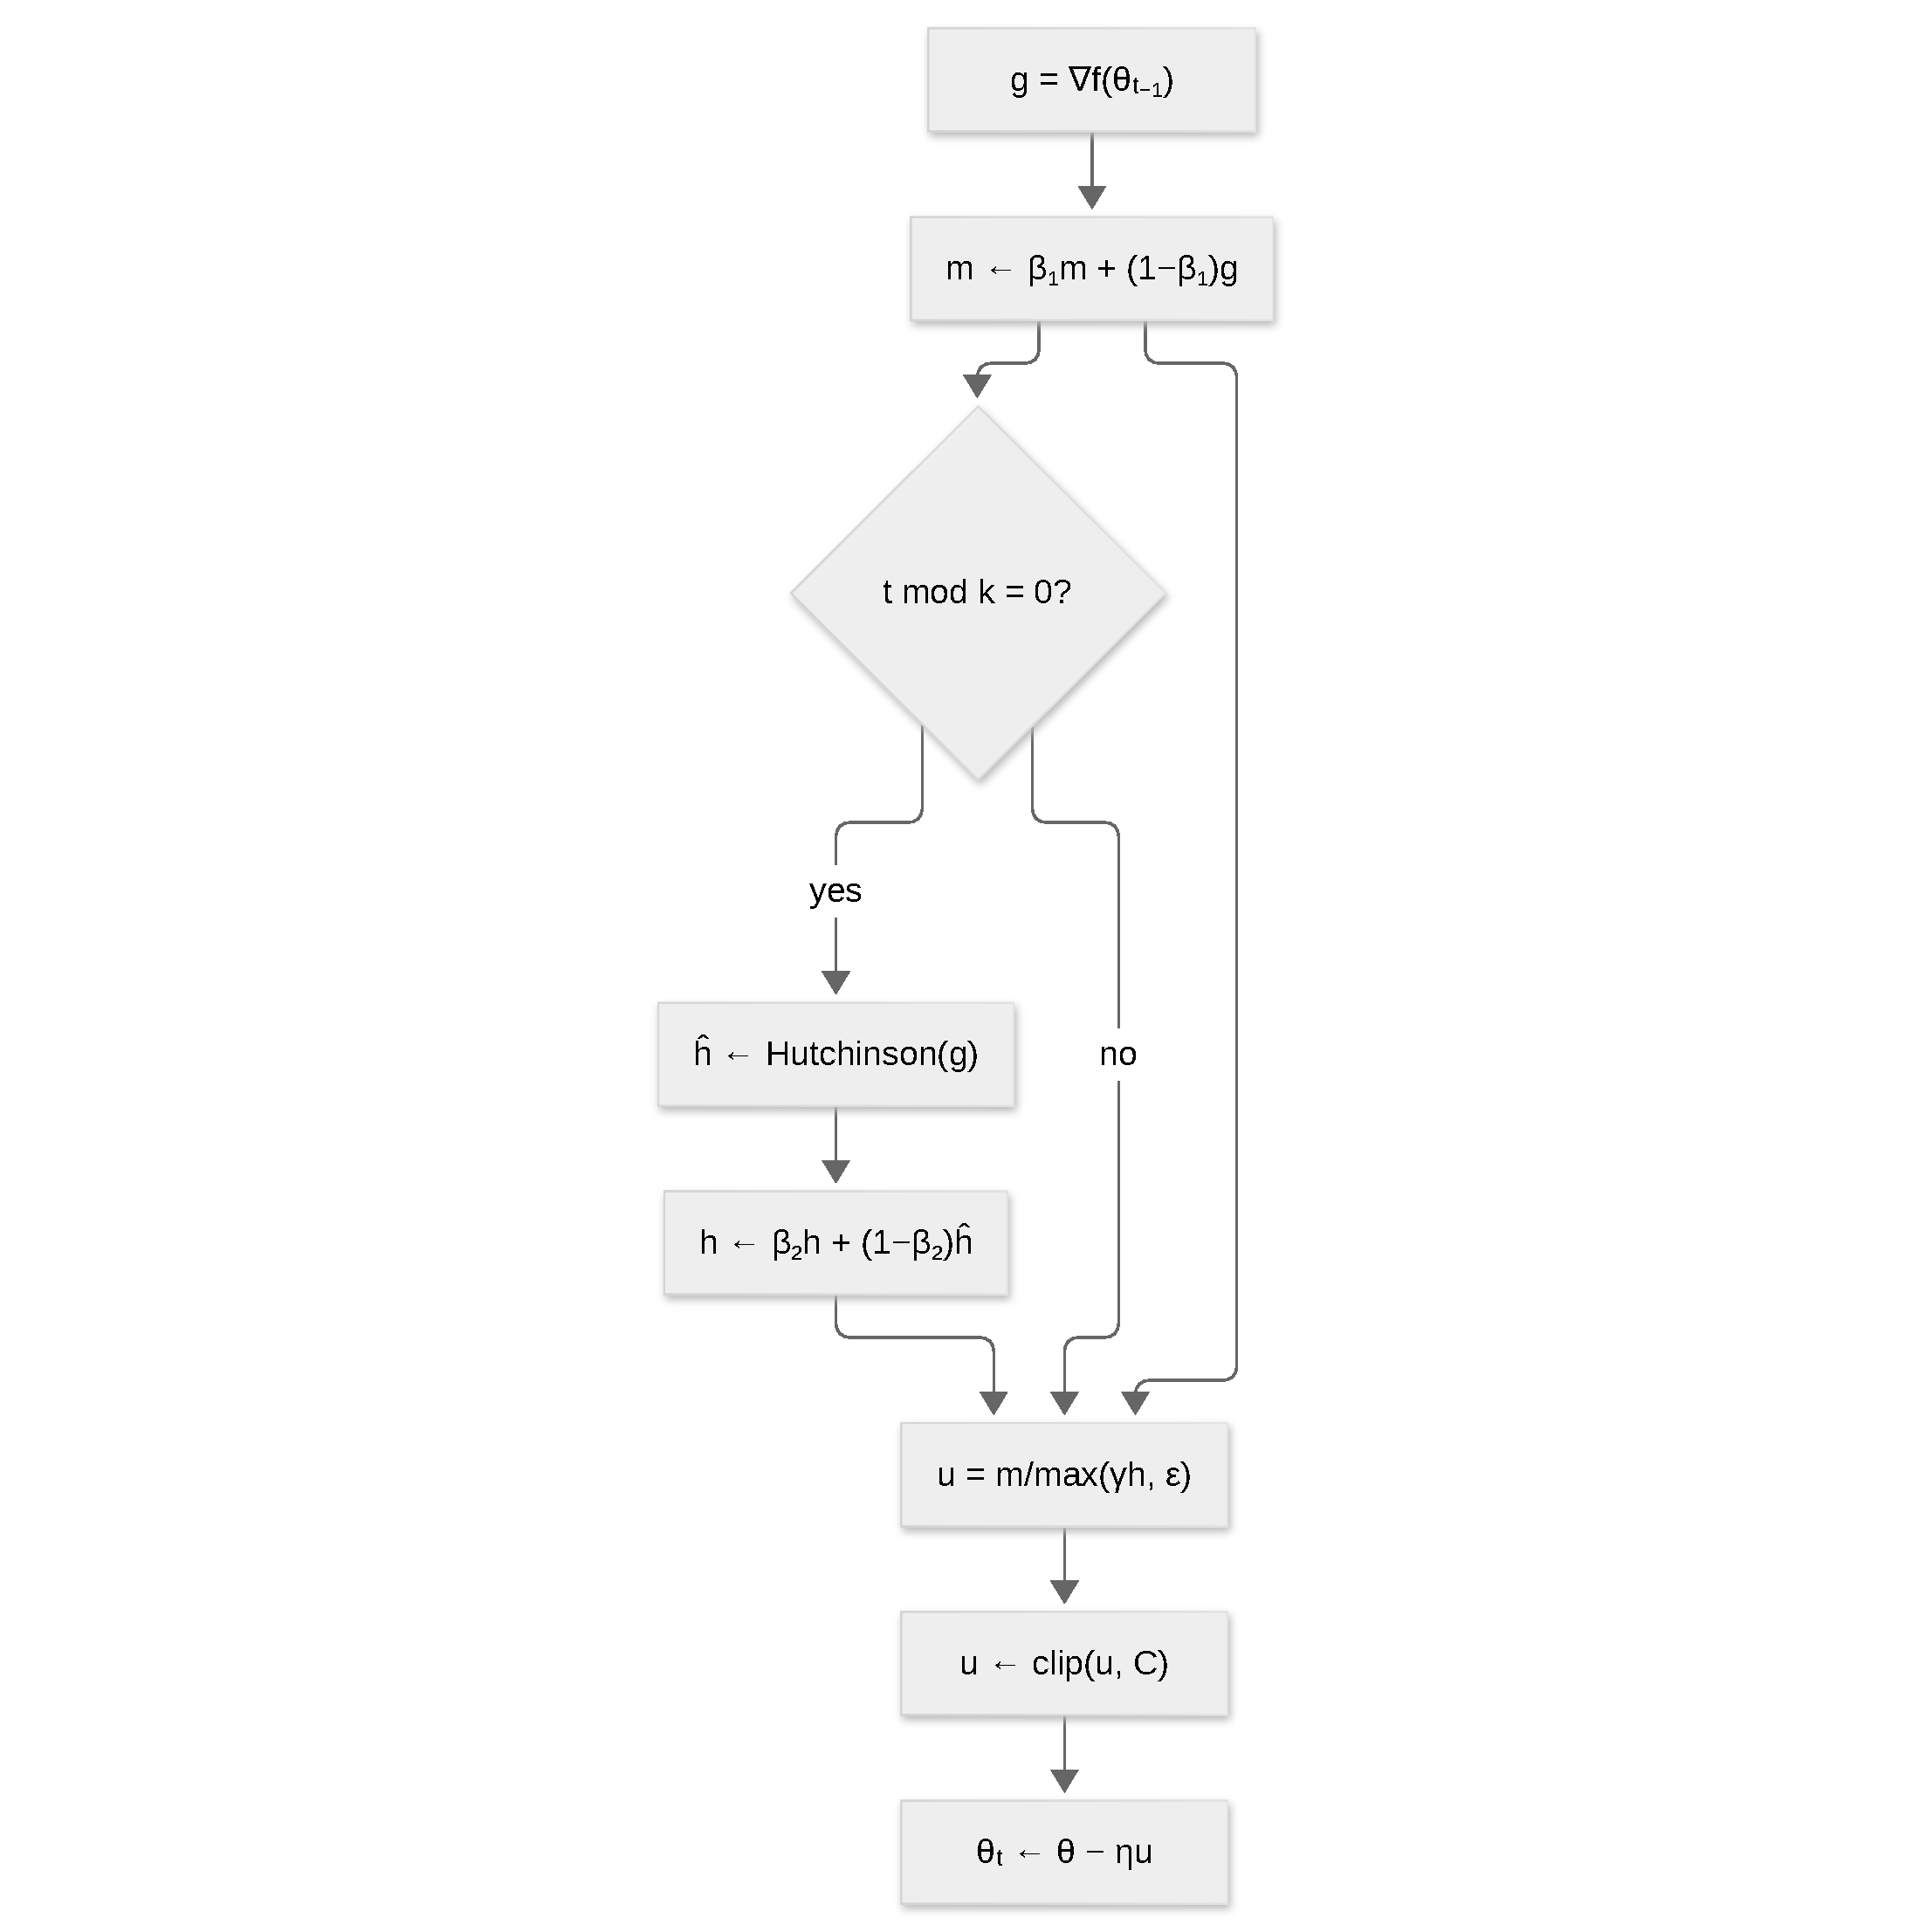
\includegraphics{../paper/figures/optimizers/sophia.pdf}}
\caption{Flujo por paso de Sophia: estimación diagonal del Hessiano mediante Hutchinson con pasos recortados conscientes de la curvatura.}
\label{fig:opt-sophia}
\end{figure}
Sophia utiliza \textbf{estimaciones diagonales del Hessiano} para escalado consciente de la curvatura sin el costo de memoria y cómputo de los métodos densos de segundo orden.
\begin{align}
m_t &= \beta_1 m_{t-1} + (1-\beta_1) g_t \quad\text{(momento de primer orden)} \\
h_t &= \beta_2 h_{t-(k-1)} + (1-\beta_2) \hat{h}_t \quad\text{(Hessiano diagonal, actualizado cada $k$ pasos)} \\
\text{clip}(x, C) &= \min(\max(x, -C), C) \quad\text{(recorte elemento a elemento)} \\
\theta_{t+1} &= \theta_t - \eta \cdot \text{clip}\left(\frac{m_t}{\max(\gamma h_t, \epsilon)}, 1\right)
\end{align}
donde $\hat{h}_t$ es una estimación diagonal (e.g., estimador de traza de Hutchinson) y $\gamma$ es un factor de escala. El Hessiano diagonal $h_t$ captura la curvatura local, permitiendo que el optimizador tome pasos más pequeños en direcciones pronunciadas y pasos más grandes en direcciones planas. La operación de recorte $\text{clip}(\cdot, 1)$ evita que los pasos adaptativos exploten.

\begin{algorithm}[H]
\caption{Sophia (Hessiano Diagonal con Actualizaciones Recortadas)}
\label{alg:sophia}
\begin{algorithmic}[1]
\Require Parámetros iniciales $\theta_0$, tasa de aprendizaje $\eta$, $\beta_1, \beta_2$, frecuencia de actualización del Hessiano $k$, umbral de recorte $C$
\Ensure Parámetros actualizados $\theta_T$
\State Inicializar: $m \gets 0$, $h \gets \epsilon$ (estimación diagonal del Hessiano)
\For{$t = 1, 2, \ldots, T$}
    \State $g \gets \nabla f(\theta_{t-1})$
    \State $m \gets \beta_1 m + (1-\beta_1) g$ \Comment{Momento de primer orden (corregir sesgo externamente)}
    \If{$t \mod k == 0$}
        \State $\hat{h} \gets \text{HutchinsonEstimate}(g)$ \Comment{Hessiano diagonal mediante Hutchinson}
        \State $h \gets \beta_2 h + (1-\beta_2) \hat{h}$ \Comment{Actualizar estimación del Hessiano}
    \EndIf
    \State $u \gets \frac{m}{\max(\gamma h, \epsilon)}$ \Comment{Paso adaptativo (elemento a elemento)}
    \State $u \gets \text{clip}(u, C)$ \Comment{Recorte elemento a elemento a $[-C, C]$}
    \State $\theta_t \gets \theta_{t-1} - \eta \cdot u$
\EndFor
\Return $\theta_T$
\end{algorithmic}
\end{algorithm}

\paragraph{Contras.}
\begin{itemize}[leftmargin=*]
\item Las estimaciones de Hutchinson añaden cómputo periódico y ruido a la señal de curvatura.
\item La estimación del Hessiano puede quedar desactualizada entre refrescos.
\end{itemize}

\paragraph{Ventajas.}
\begin{itemize}[leftmargin=*]
\item Escalado consciente de la curvatura sin el costo $O(n^2)$ u $O(n^3)$ de los métodos completos de segundo orden.
\item Los pasos recortados evitan explosiones y funcionan particularmente bien en el ajuste fino de segunda pasada.
\end{itemize}

\paragraph{Muon (Ortogonalización de Newton-Schulz).}
\begin{figure}[H]
\centering
\fitfigure{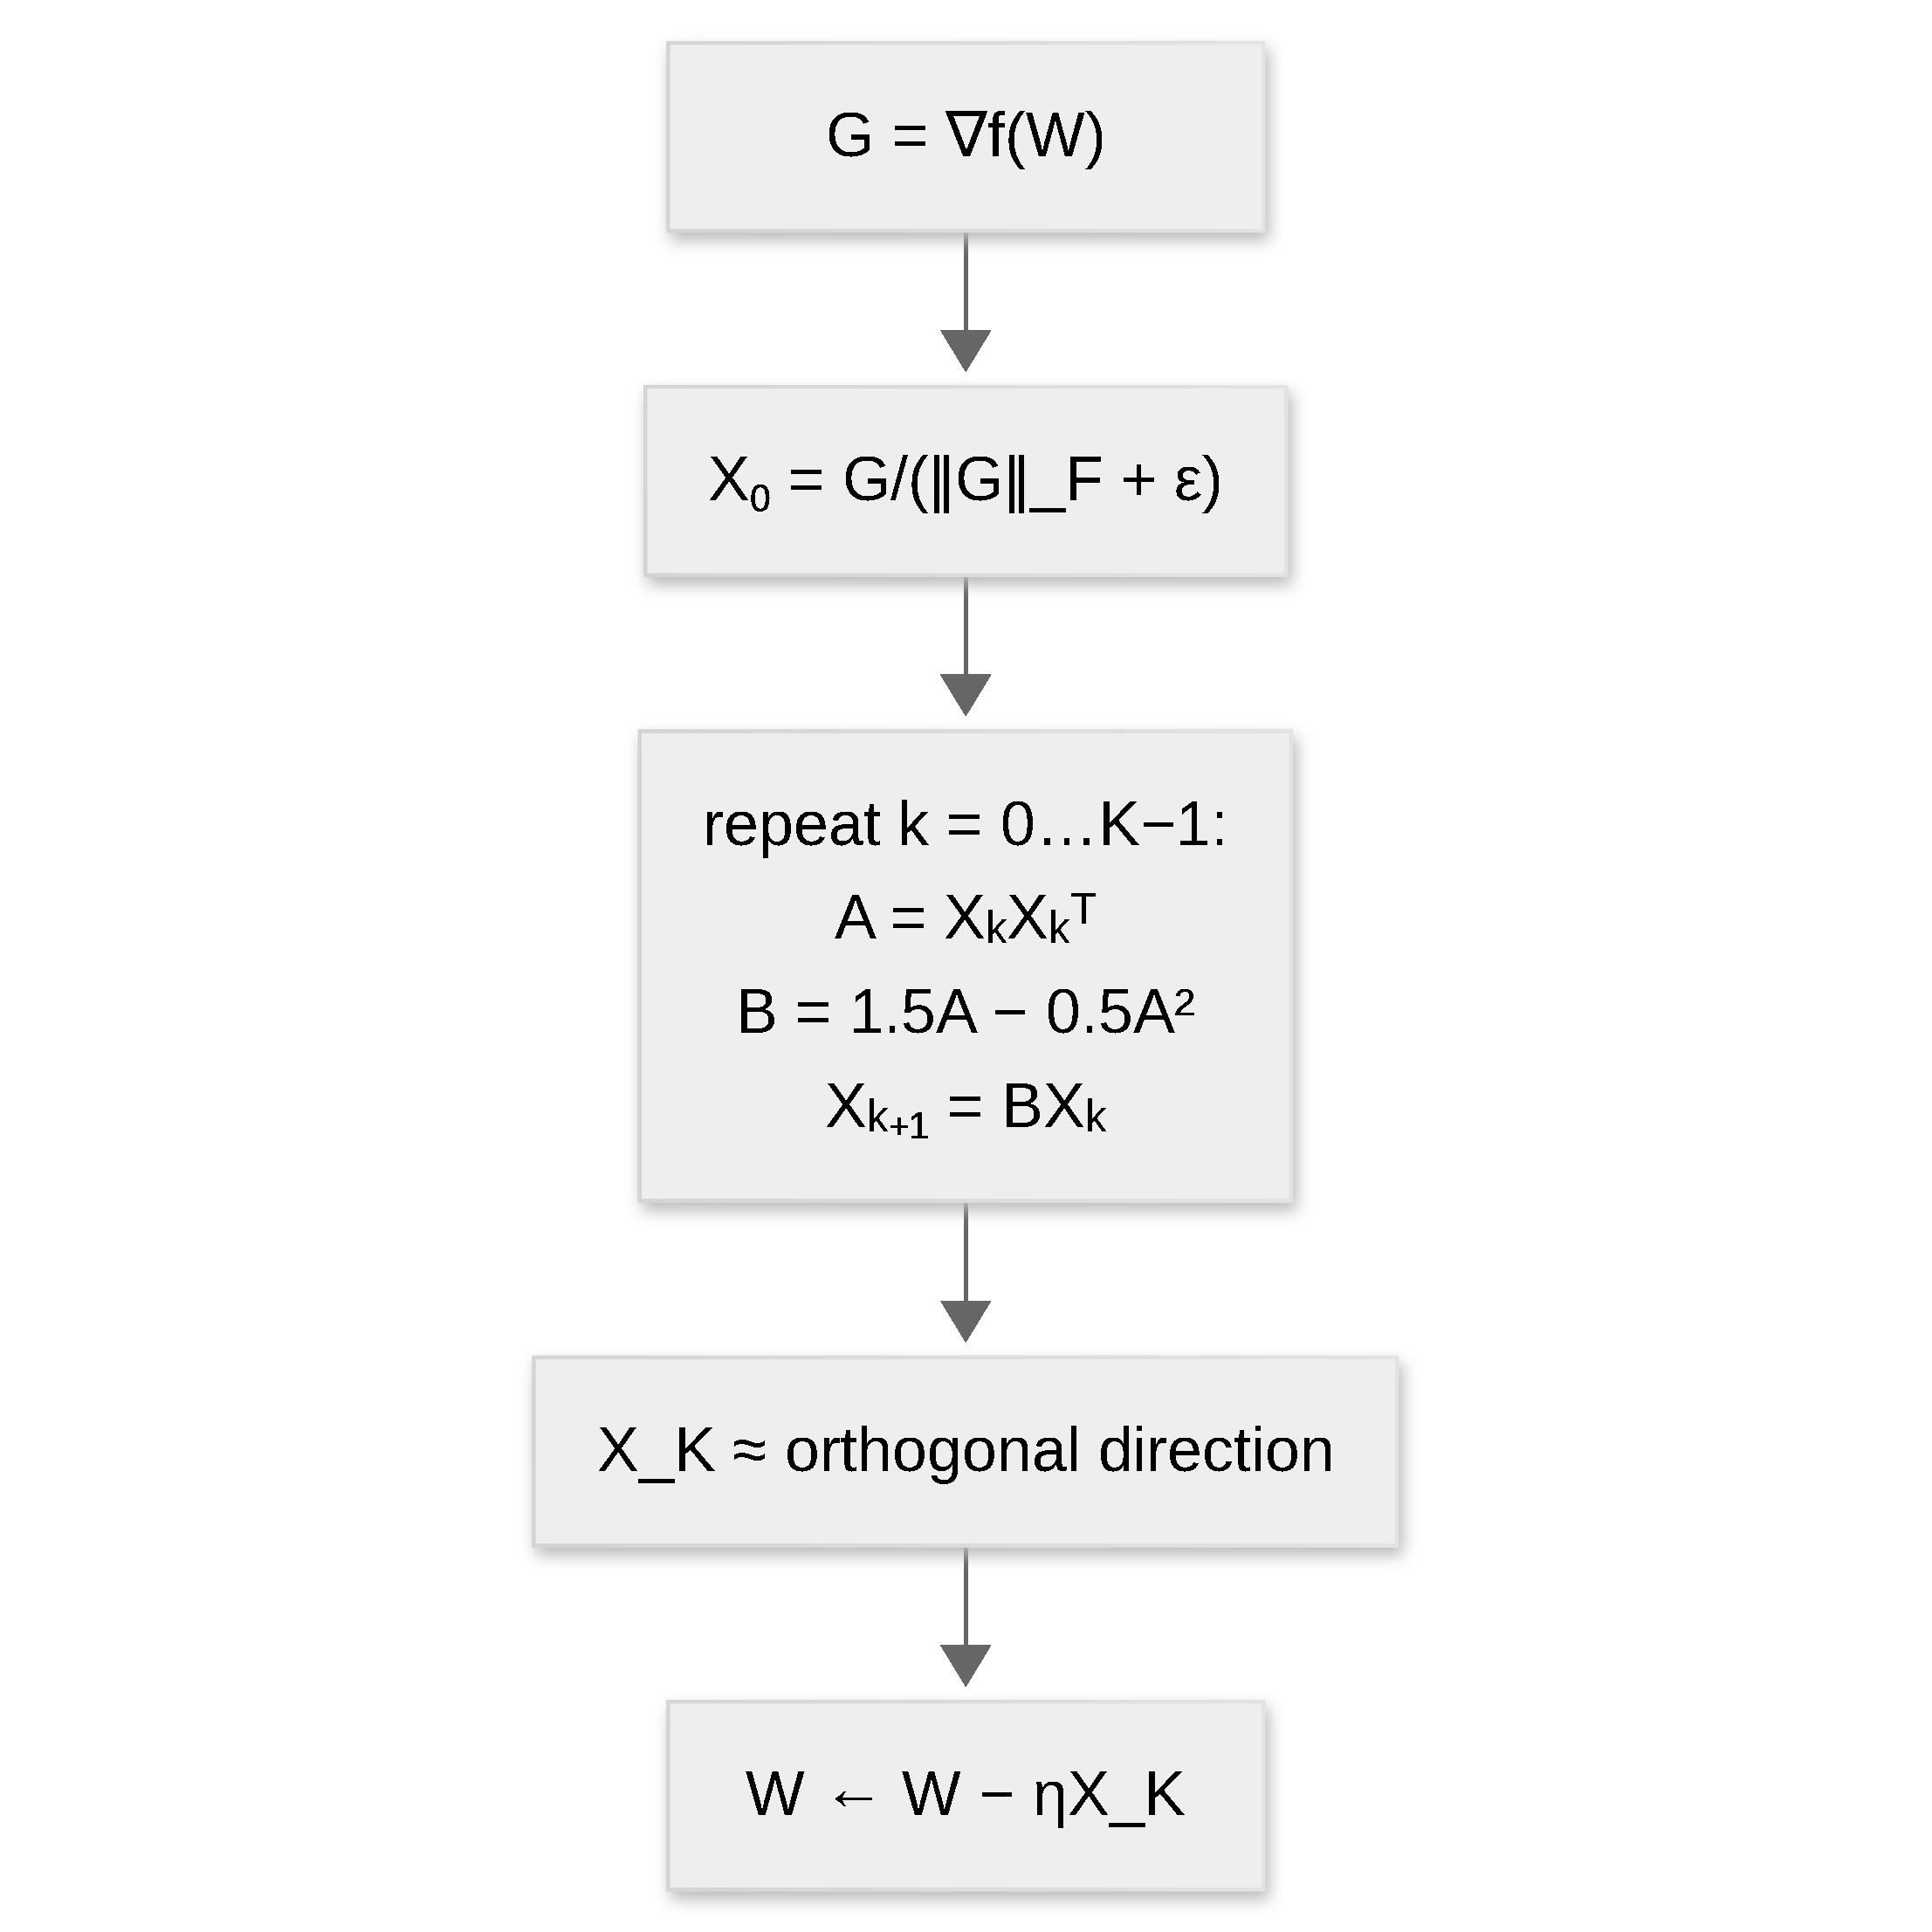
\includegraphics{../paper/figures/optimizers/muon.pdf}}
\caption{Flujo por paso de Muon: normalización de Frobenius seguida de iteraciones de Newton-Schulz que ortogonalizan la dirección de actualización.}
\label{fig:opt-muon}
\end{figure}
Muon es un \textbf{optimizador orientado a la ortogonalidad} que reformula la geometría de actualización utilizando iteraciones polinomiales de Newton-Schulz para ortogonalización. Para una matriz de parámetros 2D $W$ con gradiente $G_t$:
\begin{align}
X_0 &= \frac{G_t}{\|G_t\|_F + \epsilon} \quad\text{(gradiente normalizado)} \\
A_k &= X_k X_k^\top \quad\text{(Gramiana)} \\
B_k &= b A_k + c A_k^2 \quad\text{(paso polinomial, coeficientes $b, c$ de Newton-Schulz)} \\
X_{k+1} &= a X_k + B_k X_k \quad\text{(iteración $k=0,1,\ldots,4$)} \\
W_{t+1} &= W_t - \eta X_K \quad\text{(actualización con dirección ortogonalizada)}
\end{align}
Muon realiza 5 iteraciones de Newton-Schulz para producir una dirección aproximadamente ortogonal, asegurando que las actualizaciones respeten restricciones geométricas. La justificación: las actualizaciones ortogonales preservan las normas durante el entrenamiento, evitando la deriva de norma observada en métodos basados en momento.

\begin{algorithm}[H]
\caption{Muon (Ortogonalización de Newton-Schulz)}
\label{alg:muon}
\begin{algorithmic}[1]
\Require Parámetros iniciales $\theta$ (matrices), tasa de aprendizaje $\eta$, iteraciones Newton-Schulz $K$
\Ensure Parámetros actualizados $\theta_T$
\For{cada matriz de parámetros 2D $W$}
    \State $G \gets \nabla f(W)$ \Comment{Gradiente}
    \State $X_0 \gets \frac{G}{\|G\|_F + \epsilon}$ \Comment{Normalizar gradiente por norma de Frobenius}
    \For{$k = 0, 1, \ldots, K-1$}
        \State $A_k \gets X_k X_k^\top$ \Comment{Gramiana (costo: $O(mn^2)$ o $O(m^2n)$ para matrices altas/anchas)}
        \State $B_k \gets (3/2) A_k - (1/2) A_k^2$ \Comment{Coeficientes de Newton-Schulz}
        \State $X_{k+1} \gets B_k X_k$ \Comment{Paso polinomial}
    \EndFor
    \State $W \gets W - \eta X_K$ \Comment{Actualizar con dirección ortogonalizada}
\EndFor
\Return $\theta_T$
\end{algorithmic}
\end{algorithm}

\paragraph{Contras.}
\begin{itemize}[leftmargin=*]
\item Varias multiplicaciones de matrices por iteración de Newton-Schulz; se requieren kernels personalizados eficientes.
\item Definido solo para matrices de parámetros 2D.
\end{itemize}

\paragraph{Ventajas.}
\begin{itemize}[leftmargin=*]
\item Las actualizaciones ortogonalizadas preservan las normas y evitan la deriva de norma de los métodos basados en momento.
\item Resultados prometedores en entrenamiento a gran escala con una geometría de actualización fundamentalmente mejor condicionada.
\end{itemize}

\paragraph{Turbo-Muon (Ortogonalización Precondicionada con AOL).}
\begin{figure}[H]
\centering
\fitfigure{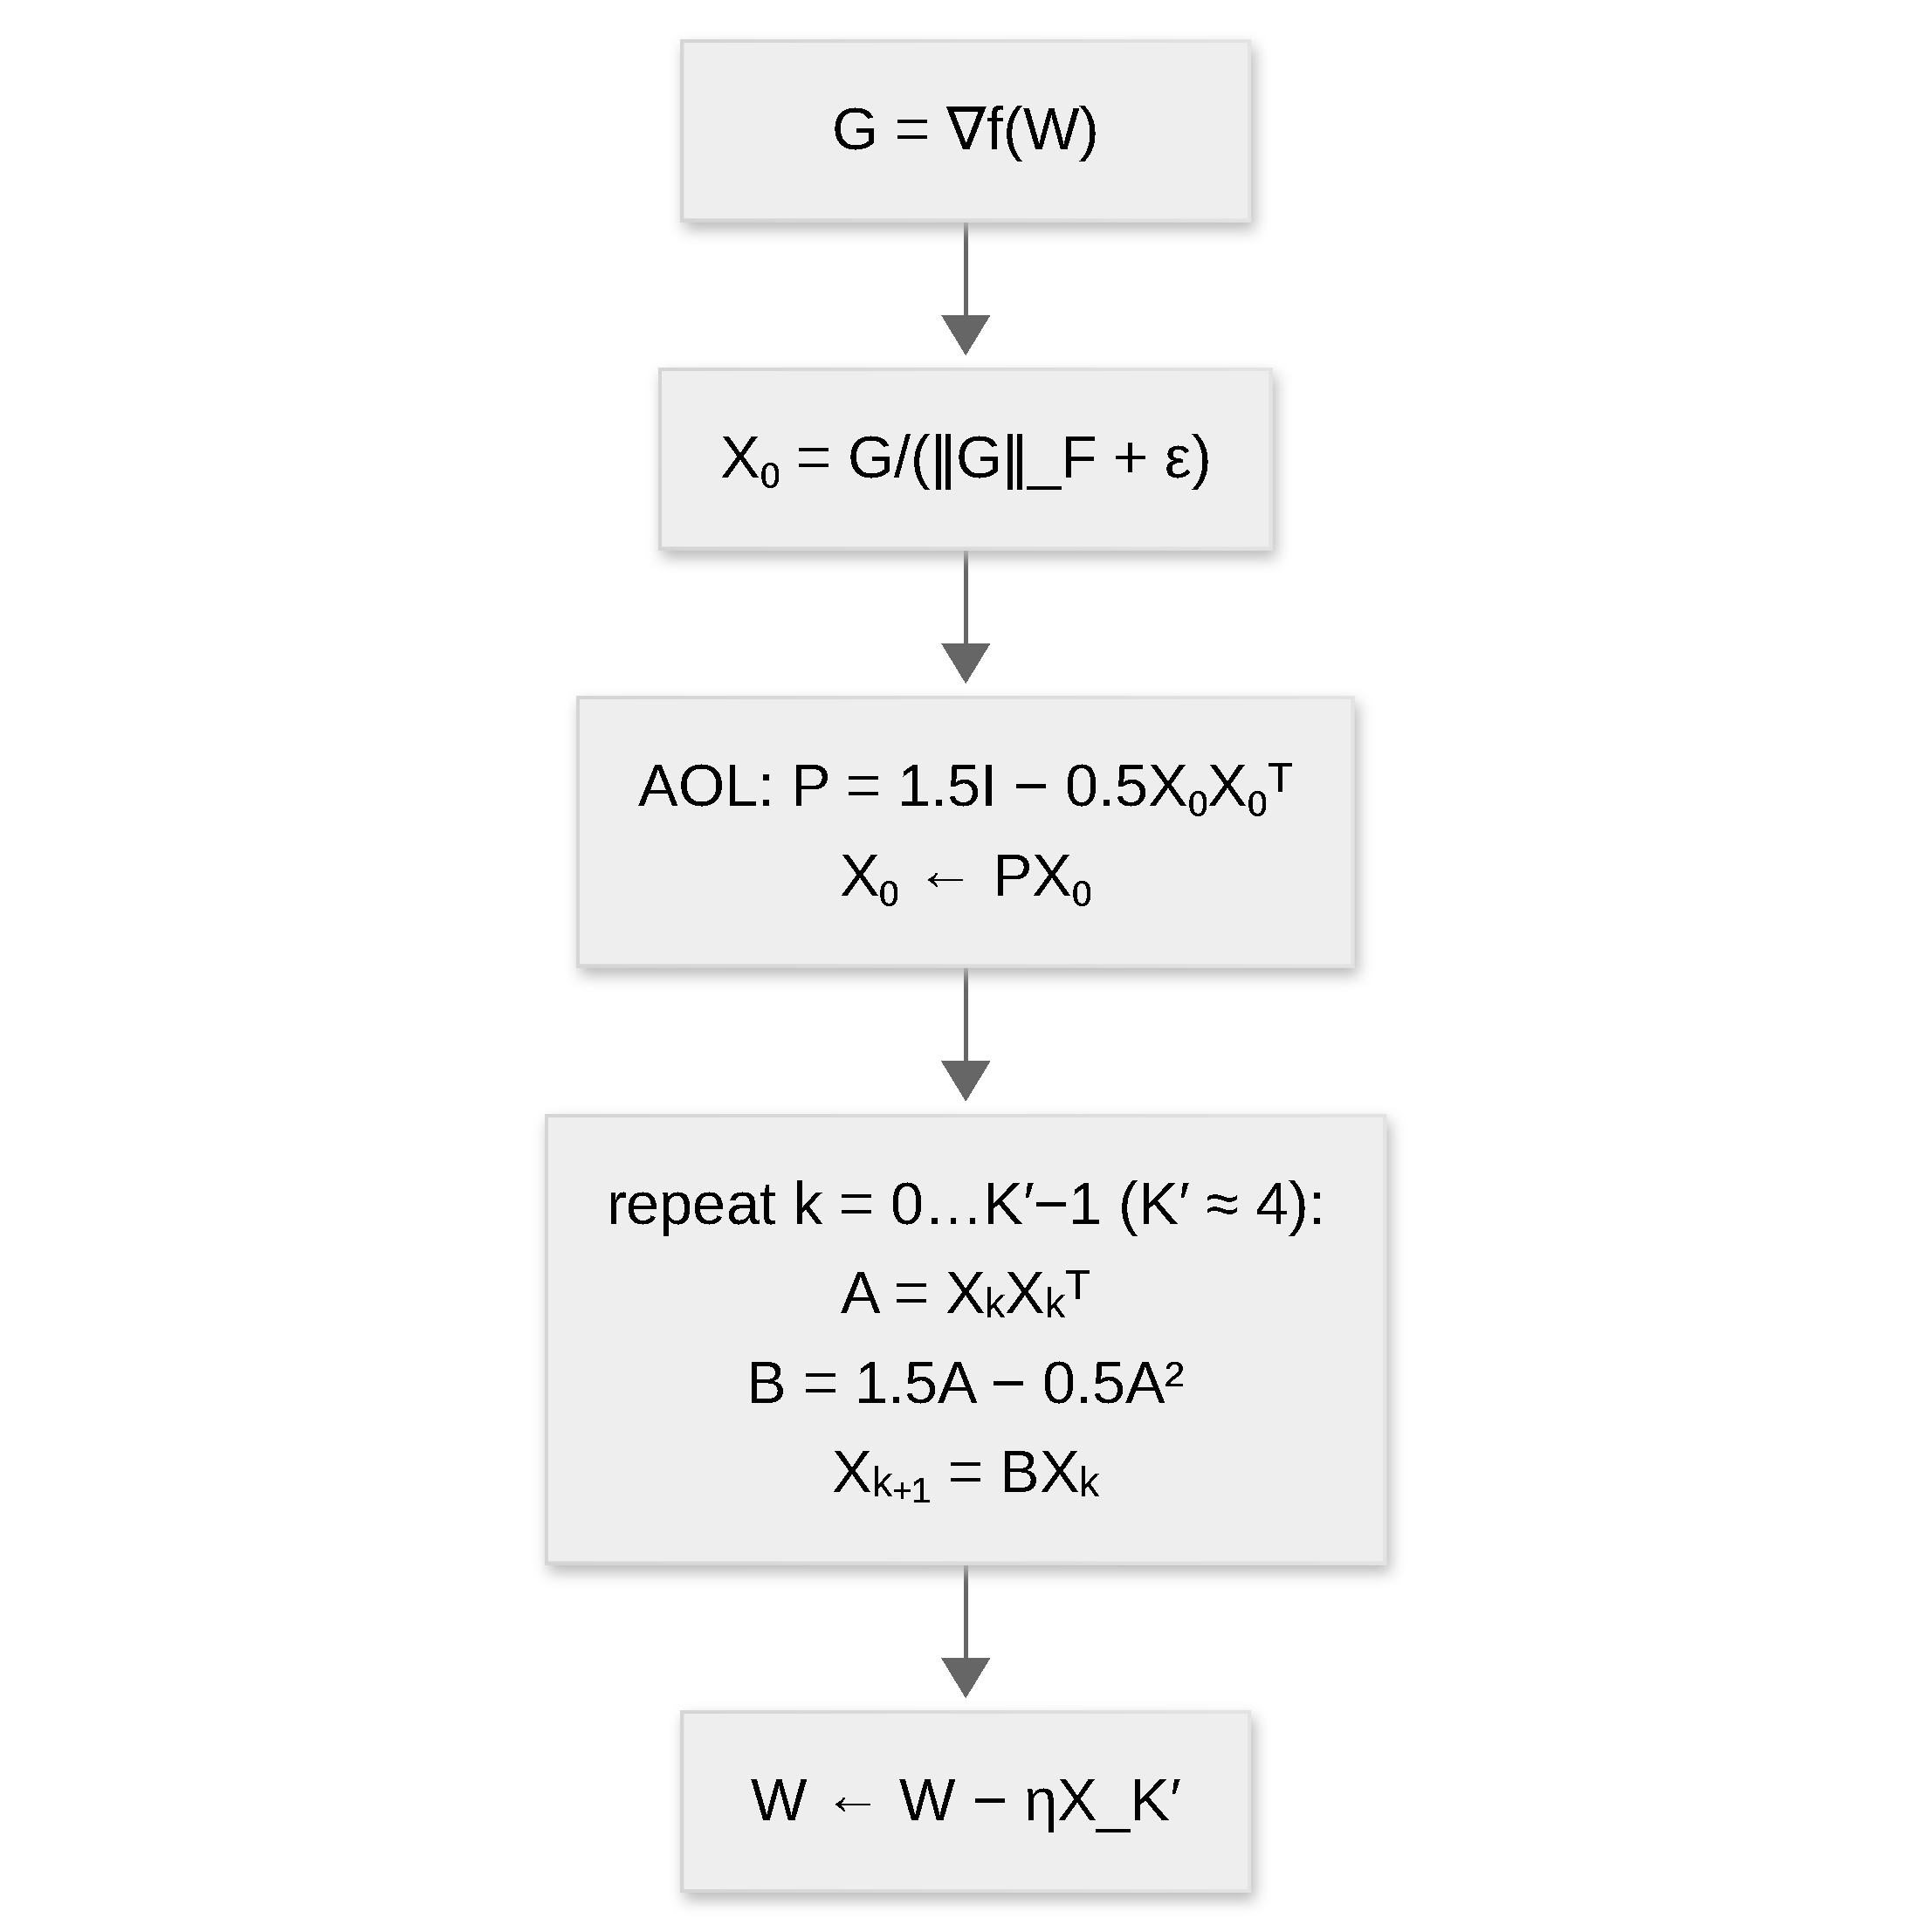
\includegraphics{../paper/figures/optimizers/turbo-muon.pdf}}
\caption{Flujo por paso de Turbo-Muon: precondicionamiento casi ortogonal (AOL) antes de las iteraciones de Newton-Schulz, reduciendo su número.}
\label{fig:opt-turbo-muon}
\end{figure}
Turbo-Muon añade un paso de \textbf{precondicionamiento casi-ortogonal} (AOL) antes de las iteraciones de Newton-Schulz. El precondicionador $P = 1.5I - 0.5X_0X_0^\top$ se aplica al gradiente normalizado, reduciendo el número de pasos de ortogonalización requeridos a cuatro mientras preserva la geometría de actualización ortogonalizada.

\begin{algorithm}[H]
\caption{Turbo-Muon (Ortogonalización Precondicionada con AOL)}
\label{alg:turbo-muon}
\begin{algorithmic}[1]
\Require Parámetros iniciales $\theta$ (matrices), tasa de aprendizaje $\eta$, iteraciones Newton-Schulz $K'$ (típicamente 4)
\Ensure Parámetros actualizados $\theta_T$
\For{cada matriz de parámetros 2D $W$}
    \State $G \gets \nabla f(W)$ \Comment{Gradiente}
    \State $X_0 \gets \frac{G}{\|G\|_F + \epsilon}$ \Comment{Normalizar gradiente}
    \State \textbf{AOL (Almost-Orthogonal preconditioner):} \Comment{Paso de precondicionamiento}
    \State $P \gets (1.5 I - 0.5 X_0 X_0^\top)$ \Comment{Matriz de precondicionamiento}
    \State $X_0 \gets P X_0$ \Comment{Inicio precondicionado}
    \For{$k = 0, 1, \ldots, K'-1$}
        \State $A_k \gets X_k X_k^\top$
        \State $B_k \gets (3/2) A_k - (1/2) A_k^2$
        \State $X_{k+1} \gets B_k X_k$ \Comment{Iteraciones reducidas gracias al precondicionamiento AOL}
    \EndFor
    \State $W \gets W - \eta X_{K'}$ \Comment{Actualizar con dirección ortogonalizada precondicionada}
\EndFor
\Return $\theta_T$
\end{algorithmic}
\end{algorithm}

\paragraph{Contras.}
\begin{itemize}[leftmargin=*]
\item Sigue siendo intensivo en cómputo; AOL añade una multiplicación de matrices de precondicionamiento.
\item Requiere el mismo soporte de kernels personalizados que Muon.
\end{itemize}

\paragraph{Ventajas.}
\begin{itemize}[leftmargin=*]
\item AOL reduce el número de iteraciones de Newton-Schulz (típicamente de cinco a cuatro).
\item Conserva la geometría de actualización ortogonalizada con menor costo de iteraciones.
\end{itemize}

\paragraph{AF-Muon (Muon sin AdamW para Vocabulario Atado).}
\begin{figure}[H]
\centering
\fitfigure{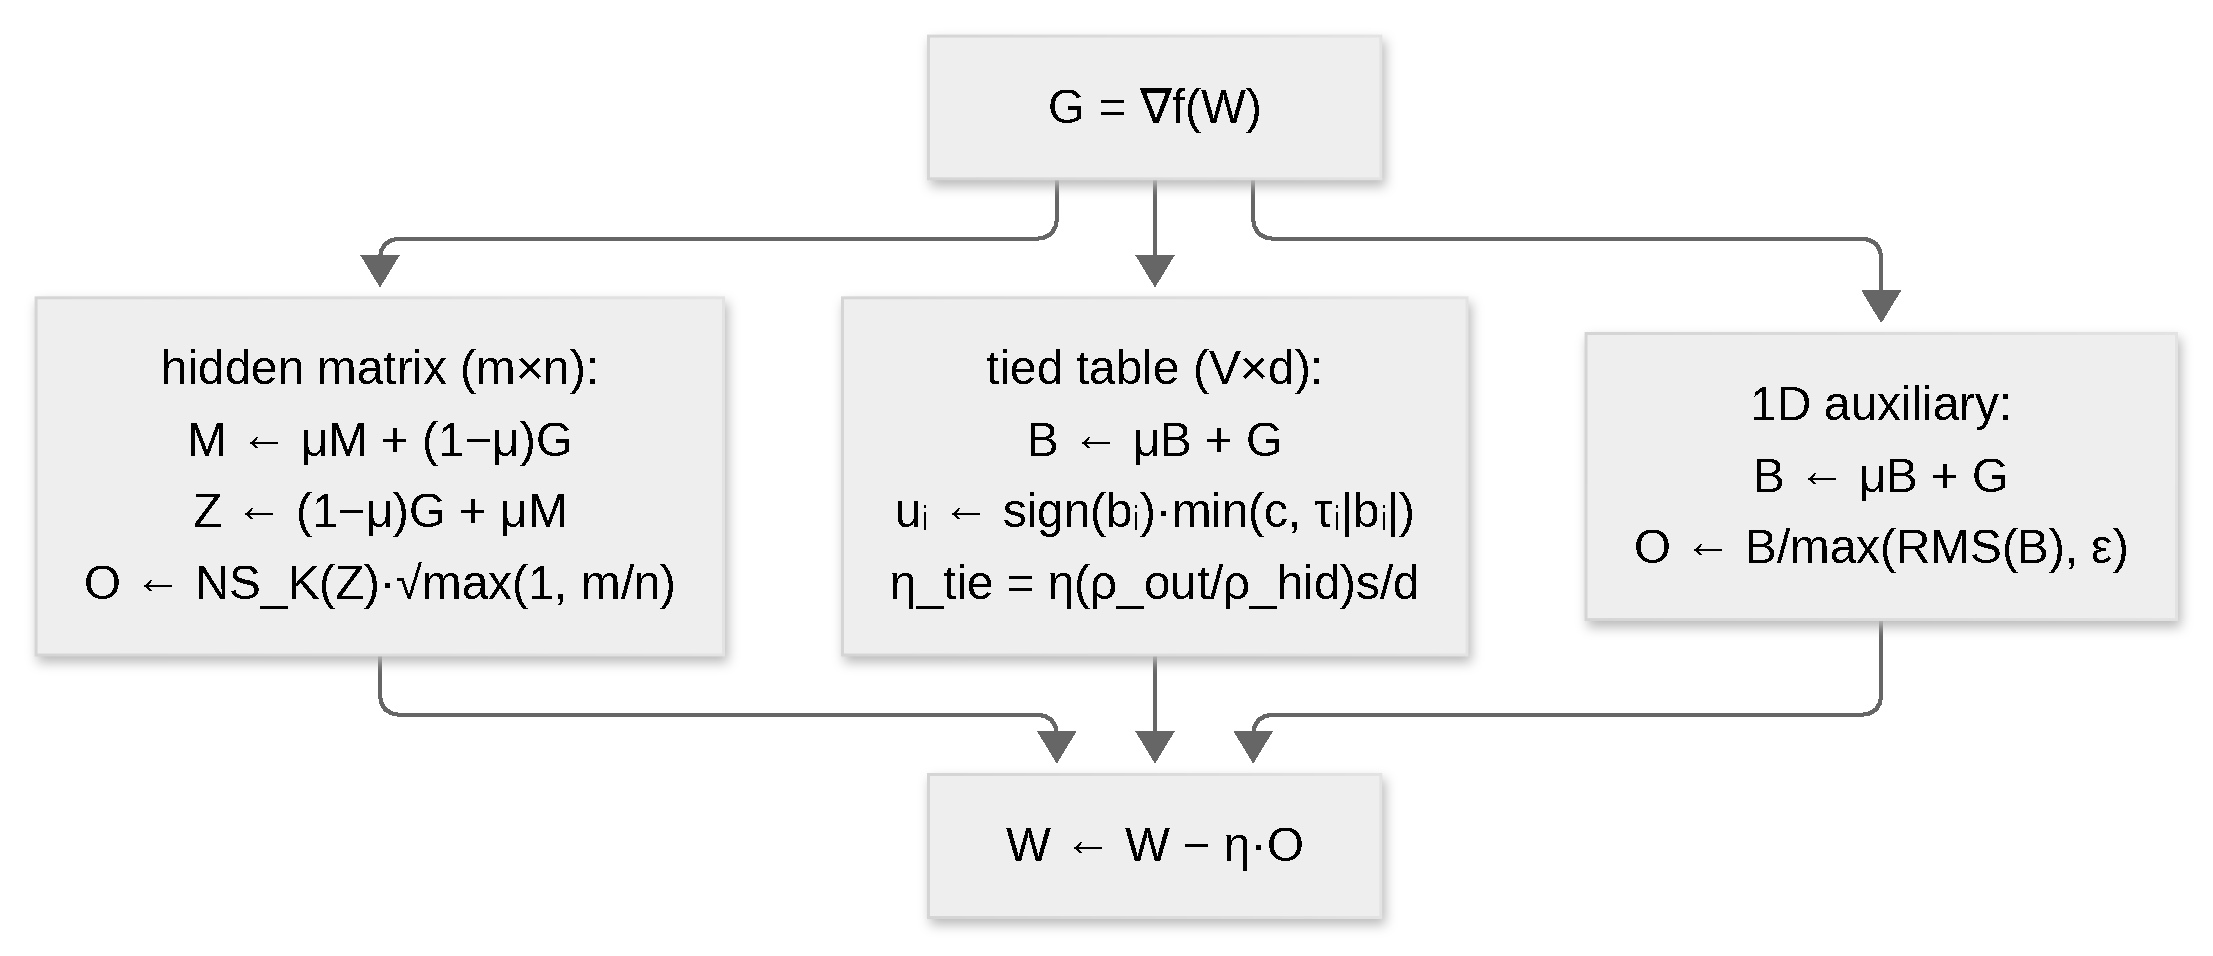
\includegraphics{../paper/figures/optimizers/af-muon.pdf}}
\caption{Flujo por paso de AF-Muon: actualización espectral de Muon para matrices ocultas, LMO por fila con tope finito y conciencia de soporte para la tabla de vocabulario atada, y actualizaciones normalizadas por RMS para parámetros auxiliares unidimensionales, todo con un único búfer de primer momento.}
\label{fig:opt-af-muon}
\end{figure}
AF-Muon es una \textbf{extensión de Muon sin AdamW} que elimina el respaldo auxiliar de AdamW de la receta Hybrid Muon asignando a cada clase de parámetro su propia geometría con restricción de norma. Las matrices ocultas conservan la actualización espectral con señal de Nesterov; la tabla de vocabulario, que recibe simultáneamente gradientes dispersos de búsqueda en la entrada y gradientes densos del softmax de salida, se actualiza fila por fila con un \emph{oráculo de minimización lineal con tope finito y conciencia de soporte}; los tensores auxiliares unidimensionales reciben una actualización normalizada por RMS. Ninguna clase de parámetro mantiene estado de segundo momento, de modo que un único búfer de primer momento por parámetro reemplaza el estado de AdamW de la receta híbrida, lo que los autores reportan como aproximadamente un 20\% menos de memoria de estado del optimizador en entrenamiento equiparado.

Para la tabla atada $W \in \mathbb{R}^{V \times d}$ con fila de momento $b_i$, el oráculo resuelve el problema por fila
\begin{align}
u_i &= \operatorname{sign}(b_i) \odot \min\left(c\,\mathbf{1},\ \tau_i\,|b_i|\right), \\
\|u_i\|_2^2 &= \min\left(d,\ c^2\,\bigl|\operatorname{supp}(b_i)\bigr|\right),
\end{align}
donde la escala por fila $\tau_i$ se obtiene por bisección en FP32 sobre fragmentos de filas completas. Las filas cuyo soporte no puede llenar el radio $\ell_2$ de fila saturan cada coordenada útil en el tope $c$, de modo que las filas dispersas de búsqueda se manejan sin inflar las coordenadas ausentes. El tope interpola entre dos extremos conocidos: $c = 1$ recupera la actualización Sign estilo SCION y $c \geq \sqrt{d}$ se reduce a una actualización row-RMS. El tamaño de paso de la tabla es $\eta_{tie} = \eta_M (\rho_{out}/\rho_{hid})\, s / d$; la configuración principal del artículo es $c = 3$ y $s = 0.5$ con $\rho_{out}/\rho_{hid} = 60$, y sus diagnósticos reportan el tope finito activo en menos del 0.3\% de las coordenadas aunque afecta a la mayoría de las filas.

\begin{algorithm}[H]
\caption{AF-Muon (Muon sin AdamW para Vocabulario Atado)}
\label{alg:af-muon}
\begin{algorithmic}[1]
\Require Parámetros iniciales $\theta$, LR de matrices $\eta_M$, LR de vectores $\eta_{vec}$, momento $\mu$, weight decay de matrices $\lambda_M$, escala de tabla $s$, tope $c$, radios $\rho_{out}, \rho_{hid}$, iteraciones Newton-Schulz $K$
\Ensure Parámetros actualizados $\theta_T$
\For{cada tensor de parámetros $W$ con gradiente $G_t$}
    \If{$W$ es una matriz oculta en $\mathbb{R}^{m \times n}$}
        \State $M_t \gets \mu M_{t-1} + (1-\mu) G_t$ \Comment{Primer momento}
        \State $Z_t \gets (1-\mu) G_t + \mu M_t$ \Comment{Señal de Nesterov}
        \State $O_t \gets \mathrm{NS}_K(Z_t)\sqrt{\max(1, m/n)}$ \Comment{Actualización espectral}
        \State $W_t \gets (1 - \eta_M \lambda_M) W_{t-1} - \eta_M O_t$
    \ElsIf{$W \in \mathbb{R}^{V \times d}$ es la tabla de vocabulario atada}
        \State $B_t \gets \mu B_{t-1} + G_t$ \Comment{Primer momento sin normalizar}
        \State $\eta_{tie,t} \gets \eta_M (\rho_{out}/\rho_{hid}) s / d$
        \For{cada fila $i = 1, \ldots, V$}
            \State $u_i \gets L_c\bigl(\mathrm{fila}_i(B_t)\bigr)$ \Comment{LMO por fila con tope}
        \EndFor
        \State $W_t \gets W_{t-1} - \eta_{tie,t} U$
    \Else
        \State $B_t \gets \mu B_{t-1} + G_t$ \Comment{Tensor auxiliar 1D}
        \State $O_t \gets B_t / \max(\mathrm{RMS}(B_t), \epsilon)$
        \State $W_t \gets W_{t-1} - \eta_{vec} O_t$
    \EndIf
\EndFor
\Return $\theta_T$
\end{algorithmic}
\end{algorithm}

\paragraph{Contras.}
\begin{itemize}[leftmargin=*]
\item Cada parámetro debe recibir un rol explícito (matriz, tabla atada o vector); un head de salida no atado o una tabla de embeddings adicional no son bloques de tabla atada.
\item El oráculo de la tabla requiere bisección por fila con fragmentación de filas completas; el artículo reporta aproximadamente un 1\% de sobrecarga mediana por paso en entrenamiento equiparado.
\item La afirmación sobre la tabla atada se establece para modelos con vocabulario atado; no se reclama preentrenamiento a escala frontera ni superioridad universal de los extremos.
\end{itemize}

\paragraph{Ventajas.}
\begin{itemize}[leftmargin=*]
\item Sin AdamW: un búfer de primer momento por parámetro y sin estado de segundo momento, reportado como aproximadamente un 20\% menos de memoria de estado del optimizador que Hybrid Muon.
\item El tope finito preserva las magnitudes intra-fila mientras acota la concentración de coordenadas, y recupera Sign ($c=1$) y row-RMS ($c \geq \sqrt{d}$) como casos límite.
\item Mejora la pérdida de validación y la perplejidad medias frente a Hybrid Muon y a un extremo Sign estilo SCION en nueve configuraciones de vocabulario atado que abarcan texto, tokens de imagen, proteínas, MoE y modelos encoder-decoder.
\end{itemize}

\paragraph{AdaMuon (Muon Adaptativo).}
AdaMuon es una \textbf{extensión adaptativa de Muon} que conserva la actualización espectral (polar) y añade normalización de varianza por coordenada. Muon ortogonaliza la matriz de momentum en una actualización puramente direccional, lo que elimina el escalado anisotrópico pero asigna la misma magnitud a todas las coordenadas; AdaMuon aborda el desajuste resultante entre coordenadas ruidosas e informativas siguiendo la varianza por elemento de la dirección \emph{ortogonalizada}, en lugar de la del gradiente crudo o la del momentum. Como el factor polar es globalmente invariante a escala, la transformación de signo aplicada antes de la ortogonalización preserva la dirección de la actualización mientras estabiliza sus magnitudes por elemento; el artículo demuestra que $\operatorname{sign}$ es la única aplicación elemental que es libre de escala, consistente con el signo, impar y acotada (Teorema~1). La estimación de segundo momento ve así una señal estable, y su versión normalizada por varianza se reescala a un RMS de $0.2$, igualando la escala empírica de actualización de Adam para reutilizar sin ajuste los schedules de tasa de aprendizaje existentes.

Para un peso $W_t \in \mathbb{R}^{n \times m}$, búfer de momentum $M_t$, momentum $\beta$, pasos de Newton--Schulz $T$ y constante pequeña $\varepsilon$:
\begin{align}
M_t &= \beta M_{t-1} + G_t, \\
O_t &= \operatorname{NewtonSchulz}\bigl(\operatorname{sign}(M_t), T\bigr), \\
V_t &= \beta V_{t-1} + (1-\beta)\, O_t \odot O_t, \\
\widehat{O}_t &= O_t \oslash \bigl(\sqrt{V_t} + \varepsilon \mathbf{1}\bigr), \\
\gamma_t &= \frac{0.2\sqrt{mn}}{\|\widehat{O}_t\|_F}, \\
W_{t+1} &= W_t - \eta\bigl(\gamma_t \widehat{O}_t + \lambda W_t\bigr).
\end{align}
El mapa de Newton--Schulz usa $X_0 = \operatorname{sign}(M_t)/\|\operatorname{sign}(M_t)\|_F$ y la iteración cúbica $X_k = aX_{k-1} + b(X_{k-1}X_{k-1}^{\mathsf T})X_{k-1} + c(X_{k-1}X_{k-1}^{\mathsf T})^2X_{k-1}$ con $(a,b,c) = (3.4445, -4.7750, 2.0315)$ y $T = 5$. No se aplica corrección de sesgo a ninguno de los momentos: un factor constante en $V_t$ se cancela exactamente con $\gamma_t \propto \sqrt{c}$, y un factor constante en $M_t$ se elimina con el mapa polar, $\operatorname{polar}(cM) = \operatorname{polar}(M)$.

\begin{algorithm}[H]
\caption{AdaMuon (Muon Adaptativo)}
\label{alg:ada-muon}
\begin{algorithmic}[1]
\Require Pesos iniciales $W_0 \in \mathbb{R}^{n \times m}$, tasa de aprendizaje $\eta$, weight decay $\lambda$, momentum $\beta$, pasos de Newton--Schulz $T$, constante pequeña $\varepsilon$
\Ensure Pesos actualizados $W_T$
\State $M_0 \gets \mathbf{0}$, $V_0 \gets \mathbf{0}$
\For{cada iteración $t = 1, 2, \ldots$}
    \State $G_t \gets \nabla_{W_t}\mathcal{L}(W_t)$
    \State $M_t \gets \beta M_{t-1} + G_t$
    \State $O_t \gets \operatorname{NewtonSchulz}(\operatorname{sign}(M_t), T)$
    \State $V_t \gets \beta V_{t-1} + (1-\beta)\, O_t \odot O_t$
    \State $\widehat{O}_t \gets O_t \oslash (\sqrt{V_t} + \varepsilon\mathbf{1})$
    \State $\gamma_t \gets 0.2\sqrt{mn}/\|\widehat{O}_t\|_F$
    \State $W_{t+1} \gets W_t - \eta(\gamma_t \widehat{O}_t + \lambda W_t)$
\EndFor
\Return $W_T$
\end{algorithmic}
\end{algorithm}

\paragraph{Contras.}
\begin{itemize}[leftmargin=*]
\item Un búfer de segundo momento adicional por parámetro matricial (dos búferes frente al único búfer de primer momento de Muon), más trabajo por paso de EMA elemental, raíz cuadrada y normalización sobre la actualización.
\item La actualización está definida para parámetros bidimensionales; los parámetros unidimensionales (sesgos, escalas de normalización) requieren un optimizador auxiliar en la receta del artículo.
\item El objetivo RMS ($0.2$) es una constante fija y no una cantidad aprendida, por lo que el método asume escalas de actualización tipo Adam al reutilizar schedules existentes.
\end{itemize}

\paragraph{Ventajas.}
\begin{itemize}[leftmargin=*]
\item Sin hiperparámetros nuevos: la EMA de segundo momento reutiliza el coeficiente de momentum $\beta$ de Muon, y el artículo reporta baja sensibilidad para $\beta \in [0.8, 0.99]$.
\item La transformación de signo hace que la estimación de varianza sea lo bastante estable para normalizar, y la alineación RMS cancela cualquier sesgo constante en $V_t$, por lo que no se necesita corrección de sesgo para ninguno de los dos momentos.
\item La alineación RMS iguala la escala de actualización de Adam, lo que permite reutilizar directamente los schedules de tasa de aprendizaje; los autores reportan hasta aproximadamente un 40\% de ganancia en eficiencia de entrenamiento frente a AdamW y mejoras consistentes frente a Muon en GPT-2 (125M--1.5B) y Qwen2.5 (1.5B, 7B).
\end{itemize}

\small
\begin{longtable}{L{2.5cm}L{3.5cm}L{2.3cm}L{5.0cm}}
\toprule
\textbf{Grupo} & \textbf{Métodos} & \textbf{Objetivo Principal} & \textbf{Interpretación desde el Estudio} \\
\midrule
\endhead
Línea base clásica & SGD, AdamW, RAdam & estabilidad y referencias base & Definen el piso de comparación para las afirmaciones de optimizadores más nuevos. \\
Rediseño de momento & Adan, AdEMAMix, MARS, Cautious AdamW & adaptación de primer orden más rápida o segura & Mejor cuando la velocidad de convergencia o la estabilidad ante gradiente ruidoso es la preocupación principal. \\
Simplificación de lotes grandes y programación & LAMB, Schedule-Free AdamW & robustez operacional a escala & Reducen la fragilidad debida al crecimiento del tamaño de lote o la ingeniería de programación. \\
Eficiencia de memoria & Adafactor, GaLore, APOLLO, APOLLO-Mini, Q-APOLLO, Lion & reducción del estado del optimizador & Más útil cuando la VRAM está dominada por el estado del optimizador en lugar de las activaciones; los métodos de la familia APOLLO reemplazan los momentos densos de AdamW con escalado estructurado proyectado o cuantizado. \\
Consciente de curvatura & Shampoo, SOAP, Sophia & mejor condicionamiento & Preferir cuando una geometría más rica justifica la sobrecarga de implementación y cómputo. \\
Orientado a geometría & Muon, Turbo-Muon, AF-Muon, AdaMuon & estructura de actualización ortogonalizada & Opciones especializadas para geometría matricial y modelado de representaciones; AdaMuon añade un segundo momento por elemento sobre la dirección ortogonalizada con actualizaciones alineadas por RMS; AF-Muon asigna a la tabla de vocabulario atada una geometría de tabla con tope por fila y a los parámetros unidimensionales una actualización RMS, sin estado auxiliar de AdamW. \\
\bottomrule
\end{longtable}
\normalsize
